% Options for packages loaded elsewhere
% Options for packages loaded elsewhere
\PassOptionsToPackage{unicode}{hyperref}
\PassOptionsToPackage{hyphens}{url}
\PassOptionsToPackage{dvipsnames,svgnames,x11names}{xcolor}
%
\documentclass[
  letterpaper,
  DIV=11,
  numbers=noendperiod]{scrartcl}
\usepackage{xcolor}
\usepackage{amsmath,amssymb}
\setcounter{secnumdepth}{-\maxdimen} % remove section numbering
\usepackage{iftex}
\ifPDFTeX
  \usepackage[T1]{fontenc}
  \usepackage[utf8]{inputenc}
  \usepackage{textcomp} % provide euro and other symbols
\else % if luatex or xetex
  \usepackage{unicode-math} % this also loads fontspec
  \defaultfontfeatures{Scale=MatchLowercase}
  \defaultfontfeatures[\rmfamily]{Ligatures=TeX,Scale=1}
\fi
\usepackage{lmodern}
\ifPDFTeX\else
  % xetex/luatex font selection
\fi
% Use upquote if available, for straight quotes in verbatim environments
\IfFileExists{upquote.sty}{\usepackage{upquote}}{}
\IfFileExists{microtype.sty}{% use microtype if available
  \usepackage[]{microtype}
  \UseMicrotypeSet[protrusion]{basicmath} % disable protrusion for tt fonts
}{}
\makeatletter
\@ifundefined{KOMAClassName}{% if non-KOMA class
  \IfFileExists{parskip.sty}{%
    \usepackage{parskip}
  }{% else
    \setlength{\parindent}{0pt}
    \setlength{\parskip}{6pt plus 2pt minus 1pt}}
}{% if KOMA class
  \KOMAoptions{parskip=half}}
\makeatother
% Make \paragraph and \subparagraph free-standing
\makeatletter
\ifx\paragraph\undefined\else
  \let\oldparagraph\paragraph
  \renewcommand{\paragraph}{
    \@ifstar
      \xxxParagraphStar
      \xxxParagraphNoStar
  }
  \newcommand{\xxxParagraphStar}[1]{\oldparagraph*{#1}\mbox{}}
  \newcommand{\xxxParagraphNoStar}[1]{\oldparagraph{#1}\mbox{}}
\fi
\ifx\subparagraph\undefined\else
  \let\oldsubparagraph\subparagraph
  \renewcommand{\subparagraph}{
    \@ifstar
      \xxxSubParagraphStar
      \xxxSubParagraphNoStar
  }
  \newcommand{\xxxSubParagraphStar}[1]{\oldsubparagraph*{#1}\mbox{}}
  \newcommand{\xxxSubParagraphNoStar}[1]{\oldsubparagraph{#1}\mbox{}}
\fi
\makeatother

\usepackage{color}
\usepackage{fancyvrb}
\newcommand{\VerbBar}{|}
\newcommand{\VERB}{\Verb[commandchars=\\\{\}]}
\DefineVerbatimEnvironment{Highlighting}{Verbatim}{commandchars=\\\{\}}
% Add ',fontsize=\small' for more characters per line
\usepackage{framed}
\definecolor{shadecolor}{RGB}{241,243,245}
\newenvironment{Shaded}{\begin{snugshade}}{\end{snugshade}}
\newcommand{\AlertTok}[1]{\textcolor[rgb]{0.68,0.00,0.00}{#1}}
\newcommand{\AnnotationTok}[1]{\textcolor[rgb]{0.37,0.37,0.37}{#1}}
\newcommand{\AttributeTok}[1]{\textcolor[rgb]{0.40,0.45,0.13}{#1}}
\newcommand{\BaseNTok}[1]{\textcolor[rgb]{0.68,0.00,0.00}{#1}}
\newcommand{\BuiltInTok}[1]{\textcolor[rgb]{0.00,0.23,0.31}{#1}}
\newcommand{\CharTok}[1]{\textcolor[rgb]{0.13,0.47,0.30}{#1}}
\newcommand{\CommentTok}[1]{\textcolor[rgb]{0.37,0.37,0.37}{#1}}
\newcommand{\CommentVarTok}[1]{\textcolor[rgb]{0.37,0.37,0.37}{\textit{#1}}}
\newcommand{\ConstantTok}[1]{\textcolor[rgb]{0.56,0.35,0.01}{#1}}
\newcommand{\ControlFlowTok}[1]{\textcolor[rgb]{0.00,0.23,0.31}{\textbf{#1}}}
\newcommand{\DataTypeTok}[1]{\textcolor[rgb]{0.68,0.00,0.00}{#1}}
\newcommand{\DecValTok}[1]{\textcolor[rgb]{0.68,0.00,0.00}{#1}}
\newcommand{\DocumentationTok}[1]{\textcolor[rgb]{0.37,0.37,0.37}{\textit{#1}}}
\newcommand{\ErrorTok}[1]{\textcolor[rgb]{0.68,0.00,0.00}{#1}}
\newcommand{\ExtensionTok}[1]{\textcolor[rgb]{0.00,0.23,0.31}{#1}}
\newcommand{\FloatTok}[1]{\textcolor[rgb]{0.68,0.00,0.00}{#1}}
\newcommand{\FunctionTok}[1]{\textcolor[rgb]{0.28,0.35,0.67}{#1}}
\newcommand{\ImportTok}[1]{\textcolor[rgb]{0.00,0.46,0.62}{#1}}
\newcommand{\InformationTok}[1]{\textcolor[rgb]{0.37,0.37,0.37}{#1}}
\newcommand{\KeywordTok}[1]{\textcolor[rgb]{0.00,0.23,0.31}{\textbf{#1}}}
\newcommand{\NormalTok}[1]{\textcolor[rgb]{0.00,0.23,0.31}{#1}}
\newcommand{\OperatorTok}[1]{\textcolor[rgb]{0.37,0.37,0.37}{#1}}
\newcommand{\OtherTok}[1]{\textcolor[rgb]{0.00,0.23,0.31}{#1}}
\newcommand{\PreprocessorTok}[1]{\textcolor[rgb]{0.68,0.00,0.00}{#1}}
\newcommand{\RegionMarkerTok}[1]{\textcolor[rgb]{0.00,0.23,0.31}{#1}}
\newcommand{\SpecialCharTok}[1]{\textcolor[rgb]{0.37,0.37,0.37}{#1}}
\newcommand{\SpecialStringTok}[1]{\textcolor[rgb]{0.13,0.47,0.30}{#1}}
\newcommand{\StringTok}[1]{\textcolor[rgb]{0.13,0.47,0.30}{#1}}
\newcommand{\VariableTok}[1]{\textcolor[rgb]{0.07,0.07,0.07}{#1}}
\newcommand{\VerbatimStringTok}[1]{\textcolor[rgb]{0.13,0.47,0.30}{#1}}
\newcommand{\WarningTok}[1]{\textcolor[rgb]{0.37,0.37,0.37}{\textit{#1}}}

\usepackage{longtable,booktabs,array}
\newcounter{none} % for unnumbered tables
\usepackage{calc} % for calculating minipage widths
% Correct order of tables after \paragraph or \subparagraph
\usepackage{etoolbox}
\makeatletter
\patchcmd\longtable{\par}{\if@noskipsec\mbox{}\fi\par}{}{}
\makeatother
% Allow footnotes in longtable head/foot
\IfFileExists{footnotehyper.sty}{\usepackage{footnotehyper}}{\usepackage{footnote}}
\makesavenoteenv{longtable}
\usepackage{graphicx}
\makeatletter
\newsavebox\pandoc@box
\newcommand*\pandocbounded[1]{% scales image to fit in text height/width
  \sbox\pandoc@box{#1}%
  \Gscale@div\@tempa{\textheight}{\dimexpr\ht\pandoc@box+\dp\pandoc@box\relax}%
  \Gscale@div\@tempb{\linewidth}{\wd\pandoc@box}%
  \ifdim\@tempb\p@<\@tempa\p@\let\@tempa\@tempb\fi% select the smaller of both
  \ifdim\@tempa\p@<\p@\scalebox{\@tempa}{\usebox\pandoc@box}%
  \else\usebox{\pandoc@box}%
  \fi%
}
% Set default figure placement to htbp
\def\fps@figure{htbp}
\makeatother


% definitions for citeproc citations
\NewDocumentCommand\citeproctext{}{}
\NewDocumentCommand\citeproc{mm}{%
  \begingroup\def\citeproctext{#2}\cite{#1}\endgroup}
\makeatletter
 % allow citations to break across lines
 \let\@cite@ofmt\@firstofone
 % avoid brackets around text for \cite:
 \def\@biblabel#1{}
 \def\@cite#1#2{{#1\if@tempswa , #2\fi}}
\makeatother
\newlength{\cslhangindent}
\setlength{\cslhangindent}{1.5em}
\newlength{\csllabelwidth}
\setlength{\csllabelwidth}{3em}
\newenvironment{CSLReferences}[2] % #1 hanging-indent, #2 entry-spacing
 {\begin{list}{}{%
  \setlength{\itemindent}{0pt}
  \setlength{\leftmargin}{0pt}
  \setlength{\parsep}{0pt}
  % turn on hanging indent if param 1 is 1
  \ifodd #1
   \setlength{\leftmargin}{\cslhangindent}
   \setlength{\itemindent}{-1\cslhangindent}
  \fi
  % set entry spacing
  \setlength{\itemsep}{#2\baselineskip}}}
 {\end{list}}
\usepackage{calc}
\newcommand{\CSLBlock}[1]{\hfill\break\parbox[t]{\linewidth}{\strut\ignorespaces#1\strut}}
\newcommand{\CSLLeftMargin}[1]{\parbox[t]{\csllabelwidth}{\strut#1\strut}}
\newcommand{\CSLRightInline}[1]{\parbox[t]{\linewidth - \csllabelwidth}{\strut#1\strut}}
\newcommand{\CSLIndent}[1]{\hspace{\cslhangindent}#1}



\setlength{\emergencystretch}{3em} % prevent overfull lines

\providecommand{\tightlist}{%
  \setlength{\itemsep}{0pt}\setlength{\parskip}{0pt}}



 


\usepackage{booktabs}
\usepackage{longtable}
\usepackage{array}
\usepackage{multirow}
\usepackage{wrapfig}
\usepackage{float}
\usepackage{colortbl}
\usepackage{pdflscape}
\usepackage{tabularx}
\usepackage{xltabular}
\usepackage{threeparttable}
\usepackage{threeparttablex}
\usepackage[normalem]{ulem}
\usepackage{makecell}
\usepackage{xcolor}
\KOMAoption{captions}{tableheading}
\makeatletter
\@ifpackageloaded{tcolorbox}{}{\usepackage[skins,breakable]{tcolorbox}}
\@ifpackageloaded{fontawesome5}{}{\usepackage{fontawesome5}}
\definecolor{quarto-callout-color}{HTML}{909090}
\definecolor{quarto-callout-note-color}{HTML}{0758E5}
\definecolor{quarto-callout-important-color}{HTML}{CC1914}
\definecolor{quarto-callout-warning-color}{HTML}{EB9113}
\definecolor{quarto-callout-tip-color}{HTML}{00A047}
\definecolor{quarto-callout-caution-color}{HTML}{FC5300}
\definecolor{quarto-callout-color-frame}{HTML}{acacac}
\definecolor{quarto-callout-note-color-frame}{HTML}{4582ec}
\definecolor{quarto-callout-important-color-frame}{HTML}{d9534f}
\definecolor{quarto-callout-warning-color-frame}{HTML}{f0ad4e}
\definecolor{quarto-callout-tip-color-frame}{HTML}{02b875}
\definecolor{quarto-callout-caution-color-frame}{HTML}{fd7e14}
\makeatother
\makeatletter
\@ifpackageloaded{caption}{}{\usepackage{caption}}
\AtBeginDocument{%
\ifdefined\contentsname
  \renewcommand*\contentsname{Table of contents}
\else
  \newcommand\contentsname{Table of contents}
\fi
\ifdefined\listfigurename
  \renewcommand*\listfigurename{List of Figures}
\else
  \newcommand\listfigurename{List of Figures}
\fi
\ifdefined\listtablename
  \renewcommand*\listtablename{List of Tables}
\else
  \newcommand\listtablename{List of Tables}
\fi
\ifdefined\figurename
  \renewcommand*\figurename{Figure}
\else
  \newcommand\figurename{Figure}
\fi
\ifdefined\tablename
  \renewcommand*\tablename{Table}
\else
  \newcommand\tablename{Table}
\fi
}
\@ifpackageloaded{float}{}{\usepackage{float}}
\floatstyle{ruled}
\@ifundefined{c@chapter}{\newfloat{codelisting}{h}{lop}}{\newfloat{codelisting}{h}{lop}[chapter]}
\floatname{codelisting}{Listing}
\newcommand*\listoflistings{\listof{codelisting}{List of Listings}}
\makeatother
\makeatletter
\makeatother
\makeatletter
\@ifpackageloaded{caption}{}{\usepackage{caption}}
\@ifpackageloaded{subcaption}{}{\usepackage{subcaption}}
\makeatother
\usepackage{bookmark}
\IfFileExists{xurl.sty}{\usepackage{xurl}}{} % add URL line breaks if available
\urlstyle{same}
% fallback for those not using the hyperref driver hyperxmp:
\makeatletter
\@ifundefined{xmpquote}{\newcommand{\xmpquote}[1]{#1}}{}
\makeatother
\hypersetup{
  pdftitle={Breeding bird indicators},
  pdfauthor={Kwaku Peprah Adjei; Katherine Rachel S. Snell; Diego Pavón-Jordán; Brett K. Sandercock},
  colorlinks=true,
  linkcolor={blue},
  filecolor={Maroon},
  citecolor={Blue},
  urlcolor={Blue},
  pdfcreator={LaTeX via pandoc}}


\title{Breeding bird indicators}
\usepackage{etoolbox}
\makeatletter
\providecommand{\subtitle}[1]{% add subtitle to \maketitle
  \apptocmd{\@title}{\par {\large #1 \par}}{}{}
}
\makeatother
\subtitle{{[}NO\_BIRD\_002{]} (Mountains)\\
{[}NO\_BIRD\_004{]} (Forests)}
\author{Kwaku Peprah Adjei \and Katherine Rachel S. Snell \and Diego
Pavón-Jordán \and Brett K. Sandercock}
\date{2026-11-11}
\begin{document}
\maketitle


\begin{figure}

\begin{minipage}[t]{0.17\linewidth}

\end{minipage}%
%
\begin{minipage}[t]{0.17\linewidth}

\end{minipage}%
%
\begin{minipage}[t]{0.17\linewidth}

\end{minipage}%
%
\begin{minipage}[t]{0.17\linewidth}

\end{minipage}%
%
\begin{minipage}[t]{0.17\linewidth}

\end{minipage}%
%
\begin{minipage}[t]{0.17\linewidth}

\end{minipage}%

\end{figure}%

\begin{quote}
\textbf{Recommended citation}: Adjei, K.P., Snell, R. S. S.,
Pavón-Jordán, D. and Sandercock, B. K. 2026. Breeding birds (ID(s):
XXX\_YYY\_ZZZ) v. 1.1.0. ecRxiv:
https://github.com/NINAnor/ecRxiv/tree/main/indicators/XX\_YYYY\_ZZZ
\end{quote}

\begin{tcolorbox}[enhanced jigsaw, arc=.35mm, bottomrule=.15mm, bottomtitle=1mm, breakable, colback=white, colbacktitle=quarto-callout-tip-color!10!white, colframe=quarto-callout-tip-color-frame, coltitle=black, left=2mm, leftrule=.75mm, opacityback=0, opacitybacktitle=0.6, rightrule=.15mm, title={Metadata}, titlerule=0mm, toprule=.15mm, toptitle=1mm]

{

\begin{longtable}[]{@{}
  >{\raggedright\arraybackslash}p{(\linewidth - 2\tabcolsep) * \real{0.2035}}
  >{\raggedright\arraybackslash}p{(\linewidth - 2\tabcolsep) * \real{0.7965}}@{}}

\caption{\label{tbl-meta2}Indicator metadata}

\tabularnewline

\toprule\noalign{}
\begin{minipage}[b]{\linewidth}\raggedright
Variable
\end{minipage} & \begin{minipage}[b]{\linewidth}\raggedright
Value
\end{minipage} \\
\midrule\noalign{}
\endhead
\bottomrule\noalign{}
\endlastfoot
Indicator ID & NO\_BIRD\_002; NO\_BIRD\_004 \\
Indicator Name & Breeding birds \\
verbatimName & VERBATIM\_INDICATOR\_NAME \\
Country & Norway \\
Continent & Europe \\
Ecosystem Condition Typology Class & B1 - Compositional State
Characteristics \\
Realm & Terrestrial (T); Terrestrial (T) \\
Biome & T2 Temperate-boreal forests and woodlands biome; T6 Polar-alpine
(cryogenic) biome \\
Ecosystem & T2.1 -- Boreal/montane forests; T6.4 -- Temperate alpine
grasslands \\
verbatimEcosystem & Forest; Mountain \\
Year added & 2026 \\
Last update & 2026 \\
Version & 1.1.0 \\
Version comment & Update of
https://github.com/NINAnor/ecRxiv/tree/main/indicators/NO\_BIRD\_001-004
bys using occupancy modelling instead of TRIM analysis. \\
Normalised & \\
Spatial aggregation pathway & Scale - Truncate - Aggregate \\
Precision & Bootstrap 95\% interval \\

\end{longtable}

}

\end{tcolorbox}

\begin{tcolorbox}[enhanced jigsaw, arc=.35mm, bottomrule=.15mm, bottomtitle=1mm, breakable, colback=white, colbacktitle=quarto-callout-tip-color!10!white, colframe=quarto-callout-tip-color-frame, coltitle=black, left=2mm, leftrule=.75mm, opacityback=0, opacitybacktitle=0.6, rightrule=.15mm, title={Log}, titlerule=0mm, toprule=.15mm, toptitle=1mm]

\begin{itemize}
\item
  15.06.2026 - Original PR
\item
  22.06.2026 - Complete draft of first version
\item
  09.11.2026 - Updating the first draft with comments from co-authors
\end{itemize}

\end{tcolorbox}

\subsection{1. Summary}\label{summary}

\begin{enumerate}
\def\labelenumi{\arabic{enumi}.}
\tightlist
\item
  \textbf{Background and rationale}:
\end{enumerate}

Birds are among the best-studied groups of organisms and a key part of
global biodiversity, so they provide extensive data for assessing
biodiversity patterns and environmental change (Barrowclough et al.
2016; Stork 1997). Because they are visible, widespread and familiar,
they are also effective for communicating environmental change to
non-specialists (Bibby 1999; Santos et al. 2026). Birds support
ecosystem functioning through seed dispersal, pollination, pest
regulation and nutrient cycling, which links them to human well-being
(Whelan et al. 2015; Mariyappan et al. 2023; Wenny et al. 2011). Bird
communities also respond to environmental variation and disturbance.
Shifts in their distributions, abundance and demographic performance
reflect land-use change, climate change, habitat degradation and changes
in food availability ({Rigal et al.} 2023; Johnson et al. 2011;
Tscharntke and Batáry 2023). This sensitivity, together with
long-running monitoring programmes, makes birds useful indicators of
environmental change.

Breeding birds are particularly informative for ecosystem assessment, as
their occurrence and reproductive performance depend closely on habitat,
resources and conditions during the breeding season (Fuller 2012;
Alerstam and Högstedt 1982). Changes in breeding bird communities can
therefore reveal variation in ecosystem composition and condition.
However, using observed occurrence or community composition as a measure
of condition requires accounting for imperfect detection, environmental
heterogeneity and natural differences in species distributions.
Occupancy models address these issues by separating the ecological
process that determines whether a species is present from the
observation process that determines whether it is detected. In addition,
species differ in prevalence and in how they respond to the environment,
so simply adding up occurrence probabilities is not enough to evaluate
condition.

In this study, we developed an occupancy-based indicator of breeding
bird community condition. We estimated occupancy probabilities for
ecologically representative breeding bird species and compared them with
expert-informed reference values defined for each species and nature
region. Standardizing occupancy against these reference values and
combining the results across species gives a spatially explicit measure
of community condition. This measure accounts for natural differences
among species and regions, so ecosystem condition can be compared across
landscapes.

\begin{enumerate}
\def\labelenumi{\arabic{enumi}.}
\setcounter{enumi}{1}
\tightlist
\item
  \textbf{Methods}:
\end{enumerate}

\begin{itemize}
\item
  \emph{Data used}: Long-term breeding-bird observations from the
  Norwegian terrestrial monitoring programme
  \href{https://hekkefuglovervakingen.nina.no/Fugl/Default.aspx?ReturnUrl=\%2fFugl\%2f}{Hekkefuglovervåkingen}
  (formerly TOV-E), spanning multiple species, ecosystems and years
  (Kålås et al. 2022).
\item
  \emph{Species selection}: Observations were restricted to
  expert-defined characteristic species for forest (32 species) and
  mountain (16 species) ecosystems. Species without an expert reference
  category were excluded from the indicator (31 forest and 14 mountain
  species remained).
\item
  \emph{Environmental covariates}: Covariates were projected and
  resampled onto a common 1 km grid (bilinear for continuous,
  nearest-neighbour for categorical variables) and extracted from the
  same raster stack at survey and prediction locations.
\item
  \emph{Occupancy modelling}: Observations were converted to
  detection/non-detection data and analysed with point-level occupancy
  models in \texttt{spOccupancy} (Doser et al. 2022), using surveys from
  2020--2024 as temporal replicates to separate detection from
  occupancy. Single- and multi-species models were fitted, with and
  without spatial effects.
\item
  \emph{Model selection}: The configuration with the lowest WAIC was
  selected for the multi-species model and for each species in the
  single-species models. Model fit was assessed with posterior
  predictive checks.
\item
  \emph{Prediction}: Occupancy was predicted at 100,000 regularly spaced
  points within forest areas (CORINE Land Cover classes 311--313) and
  mountain areas (\texttt{fjell\_grid50}).
\item
  \emph{Reference values}: Experts judged whether each species'
  occupancy under the reference condition, assuming perfect detection,
  would match or exceed its predicted occupancy. These judgements were
  linked to fixed quantiles (0.75 for \emph{same}, 0.95 for
  \emph{higher}) of predicted occupancy within each nature region,
  giving species- and region-specific reference values. Species without
  a reference category were excluded.
\item
  \emph{Scaling and aggregation}: Occupancy at each location was scaled
  linearly against its reference value and truncated to 0--1, so that
  occupancy at or above the reference value scores 1. Scaled values were
  then averaged across species. Regional estimates came from
  bootstrapped beta regressions and the national estimate from a beta
  mixed model with nature region as a random effect. Sensitivity was
  tested by varying the \emph{same} quantile from 0.5 to 0.9.
\item
  \emph{Interpretation}: Values near 1 indicate that species, on
  average, occur at or above their reference levels, while values near 0
  indicate a strong departure from the reference condition.
\end{itemize}

\begin{enumerate}
\def\labelenumi{\arabic{enumi}.}
\setcounter{enumi}{2}
\tightlist
\item
  \textbf{Interpretation}:
\end{enumerate}

An indicator value of \(1\) means that, on average, the characteristic
breeding bird species of the forest or mountain ecosystem have occupancy
probabilities at or above their expert-defined reference values for the
nature region. Values decreasing toward \(0\) indicate lower occupancy
relative to these reference values, reflecting a decline of species
expected under the reference condition. Because each species is scaled
against its own reference value before averaging, common and rare
species contribute equally. Scaled values are truncated at \(1\), so
occupancy above the reference value, or the arrival of species outside
the characteristic species list, does not raise the indicator. The
indicator is a model-based measure of condition relative to the
expert-defined reference, not a census of species present, and should be
read together with the species-specific reference values and the
sensitivity analysis.

\begin{enumerate}
\def\labelenumi{\arabic{enumi}.}
\setcounter{enumi}{3}
\tightlist
\item
  \textbf{Results and development needs}:
\end{enumerate}

The indicator expresses how closely the occupancy of characteristic
breeding bird species matches an expert-defined reference condition,
with \(1\) meaning that species occur at or above their reference levels
and \(0\) a strong departure (Table~\ref{tbl-representativeVals}).
Nationally, the indicator was \(0.67\) for forest and \(0.59\) for
mountain ecosystems. Forest ecosystems showed the largest regional
variation: values were highest in the South (\(0.74\)), similar in the
West, East and Central regions (\(0.67\)--\(0.69\)), and lowest in the
North (\(0.54\)). Mountain ecosystems showed a narrower range, from
\(0.53\) in the West and \(0.54\) in the South to \(0.64\) in the North
and East. The lower forest values in the North and at higher elevations
partly reflect natural limits on where forest birds occur, and should
not be read as degradation alone. Absolute values also depend on the
expert-based reference choice: varying it lowered the national indicator
by about \(0.09\) in forest and \(0.10\) in mountain, but the main
regional contrasts were largely unchanged
(Section~\ref{sec-sensitivity}).

The indicator can be used to compare regions and to flag where the bird
community lies further from its reference, with the caveats described in
Section~\ref{sec-uncertainties}. Model fit was poor for some widespread
species, the reported intervals only reflect resampling of locations,
and the indicator is based on a single time window (2020--2024) and
therefore cannot yet show change over time. Priorities for further
development are to (1) update the indicator as new monitoring data
become available so that trends can be assessed, (2) review the expert
reference values and the species with poor model fit, (3) include the
uncertainty of the occupancy predictions in the reported intervals, and
(4) agree guidance on how to interpret changes in indicator values in
ecosystem assessments and management.

\subsection{2. About the underlying data}\label{sec-underlyingData}

The breeding bird indicator is derived from observations collected
through the Norwegian national monitoring programme
\href{https://hekkefuglovervakingen.nina.no/Fugl/Default.aspx?ReturnUrl=\%2fFugl\%2f}{Hekkefulgovervåkingen}.
This long-term scheme provides standardized data on bird populations
across Norway and forms a common foundation for all indicator
calculations. To ensure that the indicators reflect specific ecosystem
conditions, species are selected based on expert-defined lists that
identify those most representative of each ecosystem type.

The monitoring programme was gradually established between \(2005\) and
\(2011\) and currently includes nearly \(500\) survey locations
distributed across the country. Each location consists of multiple
sampling points (typically \(12–20\)), and most sites are surveyed
annually. Data collection is carried out largely by trained volunteer
observers following a
\href{https://hekkefuglovervakingen.nina.no/Fugl/public/papirskjema/MethodologyEng.pdf}{standardized
protocol}, ensuring consistency across regions and years. Surveys are
conducted once per year during the main breeding season (late May to
early June), under suitable weather conditions.

At each sampling point, observers record all birds seen or heard within
a fixed time period, while additional observations of selected species
are noted during movement between points. The dataset typically includes
records of over \(200\) bird species. All observations are
quality-checked and stored in a central
\href{https://hekkefuglovervakingen.nina.no/Fugl/Default.aspx}{database}
managed by NINA.

\subsubsection{2.1 Spatial and temporal resolution and
extent}\label{spatial-and-temporal-resolution-and-extent}

The indicator is based on data from the Norwegian breeding bird
monitoring programme (Hekkefuglovervåkingen), which covers terrestrial
ecosystems across the entire country. The monitoring network consists of
\(492\) fixed survey routes distributed along major latitudinal and
altitudinal gradients, providing broad ecological representation. Each
route includes \(12–20\) point-count locations, resulting in
approximately \(9,000\) sampling points nationwide.

For this ecological indicator, data from \(2020\) to \(2024\) were used,
providing a recent and consistent time window. The temporal resolution
is annual, as each route is surveyed once during the breeding season.
Due to logistical constraints, around \(370\) routes are sampled each
year, ensuring coverage of roughly \(80\%\) of the total network.

The indicator is aggregated at the regional and national scale,
reflecting the overall ecosystem condition across Norway.

\subsubsection{2.2 Sampling design}\label{sampling-design}

Bird data are collected using a standardized point-count survey design.
Each route consists of a sequence of predefined counting points,
typically spaced about 300 m apart and often arranged in a square-shaped
layout (ca. \(1.5\) km per side). At each point, observers record all
birds seen or heard within a fixed observation period (\(5\) minutes).
In addition, selected species that are harder to detect are recorded
while moving between points.

Surveys are conducted once per year during the peak breeding season
(late May to early June), under suitable weather conditions. Data
collection is largely carried out by experienced volunteer observers
following a consistent protocol, ensuring comparability across sites and
years.

Potential sources of sampling bias include variation in observer skill,
uneven annual coverage of routes, and limitations in accounting for
spatial structure in analyses. Furthermore, some habitats may be
underrepresented due to accessibility constraints or terrain, which can
influence detection probabilities and species representation.

\subsubsection{2.3 Original units}\label{original-units}

During field surveys, observers record the number of individuals of each
species seen or heard at each sampling point. For this indicator, these
counts were converted to detection/non-detection data: a species was
coded as detected (1) if one or more individuals were recorded at a
sampling point in a given year, and as not detected (0) otherwise.
Because each point is surveyed once per year, the surveys from
2020--2024 were treated as repeated survey occasions, assuming that
occupancy did not change over this period.

\textbf{ADD DATAFRAME OF DATASET ENCOUNTER HISTORIES FOR SOME OF THE
SPECIES.}

This transformation gives a standardized response suited to occupancy
modelling and shifts the focus from the number of individuals to whether
a species is present. The count data contain many zeros, particularly
for rare species. Detection/non-detection data are less sensitive to
this and to variation in flock size than the raw counts. The repeated
surveys allow the models to separate the probability that a species
occupies a site from the probability that it is detected when present.
The detection/non-detection data were analysed with point-level
occupancy models to estimate species-specific occupancy probabilities,
corrected for imperfect detection. These probabilities were then
predicted across each ecosystem, scaled against species- and
region-specific reference values, and averaged across species to produce
the ecosystem-level ecological indicator.

\subsubsection{2.4 Instructions for citing, using and accessing
data}\label{instructions-for-citing-using-and-accessing-data}

The data are publicly available on
\href{https://www.gbif.org/dataset/4a00502d-6342-4294-aad1-9727e5c24041}{GBIF}
(Stokke et al. 2026).

\subsubsection{2.5 Additional comments about the
dataset}\label{additional-comments-about-the-dataset}

\emph{Diego can help with this}

\subsection{3. Indicator properties}\label{indicator-properties}

The ecological indicator was calculated as the mean of species-specific
occupancy probabilities, adjusted for imperfect detection (\(p < 1\))
through occupancy modelling and subsequently scaled against
expert-elicited, species-specific reference values defined for each
nature region. Specifically, the indicator at location \(j\) was
calculated as

\[
I_j = \frac{1}{S_j}\sum_{s=1}^{S_j} \min\left(1,\frac{\psi_{sj}}{\psi^{\mathrm{ref}}_{sr}}\right),
\]

where \(S_j\) is the number of species included at location \(j\),
\(\psi_{sj}\) is the estimated occupancy probability of species \(s\) at
location \(j\), and \(\psi^{\mathrm{ref}}_{sr}\) is the expert-informed
reference occupancy value (\(x_{100}\)) for species \(s\) in nature
region \(r\), with \(j\) located in region \(r\).

This approach accounts for species-specific differences in detectability
and natural occupancy patterns while placing all species on a common
scale ranging from 0 to 1. By averaging the reference-scaled occupancy
probabilities, each species contributes equally to the indicator,
irrespective of its natural prevalence. Consequently, both common and
rare species can contribute to the assessment of ecosystem condition
without the indicator being dominated by naturally widespread species.

\subsubsection{3.1 Ecosystem Condition Typology Class
(ECT)}\label{ecosystem-condition-typology-class-ect}

B1 -- Compositional state characteristics.

\subsubsection{3.1.1 Other condition
typologies}\label{other-condition-typologies}

\subsubsection{3.2 Ecosystem condition
characteristic}\label{ecosystem-condition-characteristic}

The indicator represents the ecosystem characteristic \emph{intact
breeding bird community composition} and belongs to the compositional
state class (biotic) of the SEEA Ecosystem Condition Typology (Czúcz et
al. 2021). It describes how closely the occupancy of characteristic
breeding bird species in forest and mountain ecosystems approaches their
expert-defined reference levels. High values indicate that
characteristic species occupy the landscape at or near reference levels.
Lower values indicate that characteristic species are reduced or
missing, which reflects a departure from the reference condition.

\subsubsection{3.3 Collinearities with other
indicators}\label{collinearities-with-other-indicators}

The breeding bird indicator may be correlated with other indicators of
biodiversity and ecosystem condition because species-specific occupancy
probabilities are predicted using environmental covariates, including
habitat characteristics, topography and climate. Consequently,
correlations with habitat-based indicators may partly reflect shared
predictors rather than independent ecological responses. The indicator
may also correlate with other bird-based indicators derived from the
same monitoring data and with broader measures of ecosystem integrity
(Nater et al. 2025). However, unlike conventional richness or abundance
indicators, it uses species-specific occupancy probabilities scaled
against expert-elicited reference values within nature regions, allowing
common and rare species to contribute on a comparable scale.
Correlations with indicators for other taxa may also occur where species
respond to similar environmental gradients. Such overlap should be
considered when combining indicators to avoid redundancy and
disproportionate weighting of particular ecosystem attributes.

\subsubsection{3.4 Impact factors}\label{impact-factors}

The breeding bird indicator is influenced by a range of natural and
human-driven factors that affect bird communities and their habitats.

\begin{itemize}
\item
  Natural factors:

  \begin{itemize}
  \tightlist
  \item
    Climate variability (e.g.~temperature, precipitation, and seasonal
    timing), which affects breeding success, migration, and food
    availability
  \item
    Habitat heterogeneity and natural succession, influencing vegetation
    structure and nesting opportunities
  \item
    Natural fluctuations in food resources, particularly insects and
    seeds
  \item
    Predation and interspecific interactions, which can shape species
    presence and community composition
  \end{itemize}
\item
  Anthropogenic factors:

  \begin{itemize}
  \tightlist
  \item
    Land-use change (e.g.~forestry, agriculture, urbanization), leading
    to habitat loss, fragmentation, or alteration
  \item
    Climate change, altering species distributions, phenology, and
    ecosystem dynamics
  \item
    Changes in land management practices, such as intensification or
    abandonment
  \item
    Pollution and other environmental pressures that affect habitat
    quality and food resources.
  \end{itemize}
\end{itemize}

Together, these drivers influence species occupancy and richness, making
the indicator sensitive to both gradual environmental change and more
abrupt disturbances.

\subsubsection{3.5 Spatial aggregation}\label{spatial-aggregation}

Scaling is performed separately for each species at each prediction
location, before aggregation. Species-specific occupancy probabilities
are linearly scaled against expert-elicited reference values defined for
each species and nature region, with a lower bound of 0 and truncation
at 1. The scaled values are then aggregated using an unweighted
arithmetic mean across species at each location, producing an indicator
ranging from 0 to 1.

Regional estimates are obtained by fitting intercept-only beta
regression models to bootstrap samples of the location-level indicator
values within each nature region. The national estimate is derived from
a beta mixed-effects model with nature region as a random effect,
representing the expected condition of a typical region rather than an
area-weighted national mean. Values of exactly 0 or 1 are adjusted to
fall within the open interval (0, 1) before model fitting. The final
point estimates are calculated as the means of the bootstrap estimates,
with 95\% bootstrap intervals obtained from their 2.5th and 97.5th
percentiles.

\subsection{4. Reference condition and
levels}\label{reference-condition-and-levels}

\subsubsection{4.1 Reference condition}\label{reference-condition}

Following Keith et al. (2020), we distinguish between the
\emph{reference condition}, representing the ecological state against
which ecosystem condition is assessed, and \emph{reference levels},
representing the numerical indicator values associated with that
condition. The reference condition was defined as the expected occupancy
of characteristic breeding bird species in forest and mountain
ecosystems under good ecological condition, based on expert judgement.
Experts assessed whether species occupancy under reference conditions,
assuming perfect detection, would be similar to or higher than the
model-estimated mean occupancy probabilities.

Expert assessments were translated into species-specific reference
levels using predefined quantiles of predicted occupancy probabilities
(0.75 for \emph{same} and 0.95 for \emph{higher}). Reference levels were
calculated separately for each species and nature region to account for
natural variation in occupancy across species and environmental
gradients. Species without expert-defined reference categories were
excluded. This approach provides a consistent reference framework
without requiring undisturbed reference sites. However, because
reference levels depend on expert judgement and model predictions, we
assessed the sensitivity of the indicator by varying the quantile
assigned to the \emph{same} category from 0.50 to 0.90.

\subsubsection{4.2 Reference levels}\label{reference-levels}

The variable normalised is the predicted occupancy probability
(\(\hat{\psi}_{sj}\)) of each characteristic breeding bird species \(s\)
at prediction location \(j\). Normalisation is performed separately for
each species and nature region using two reference levels.
\textbf{X\textsubscript{0} (worst condition)} is set to 0, representing
species absence, while \textbf{X\textsubscript{100} (reference
condition)} represents the species- and region-specific occupancy
reference value derived from expert judgement. Experts assessed whether
occupancy under reference conditions would be similar to or higher than
model-estimated occupancy. These assessments were translated into the
0.75 (\emph{same}) and 0.95 (\emph{higher}) quantiles of predicted
occupancy within each nature region. No intermediate anchoring points
(X\textsubscript{n}) were used.

Occupancy probabilities are linearly scaled between X\textsubscript{0}
and X\textsubscript{100}, with values truncated at 1 when predicted
occupancy equals or exceeds the reference level. The resulting scaled
values are averaged across species at each prediction location to obtain
the indicator. Defining reference levels separately for each species and
nature region accounts for natural differences in occupancy and allows
common and rare species to contribute on a comparable scale.
Expert-informed reference levels were preferred over protected areas as
proxies for reference conditions because protected status does not
necessarily indicate good ecological condition. Since reference levels
depend on the selected quantiles of model predictions, sensitivity was
assessed by varying the quantile assigned to the \emph{same} category
from 0.50 to 0.90.

\paragraph{4.2.1 Spatial resolution and
validity}\label{spatial-resolution-and-validity}

The reference levels vary spatially. Experts gave one reference category
per species for the whole of Norway, but the reference level is
calculated separately for each nature region as the corresponding
quantile of the species' predicted occupancy within that region. Each
species therefore has one reference level per nature region, which is
constant within the region and differs between regions. This accounts
for natural differences in occupancy along environmental gradients.
Scaling is applied at the level of individual prediction locations,
using the reference level for the nature region in which the location
falls. The scaled values are then averaged across species and aggregated
to regional and national estimates without recalculating the reference
levels. Locations outside all nature regions have no reference level and
are excluded.

\subsection{5. Uncertainties}\label{sec-uncertainties}

\subsubsection{5.1 General uncertainties}\label{general-uncertainties}

Several sources of uncertainty affect the interpretation of the breeding
bird indicator. Reference levels are derived from expert judgements
translated into predefined quantiles of model-predicted occupancy within
each nature region. Consequently, indicator values depend on both expert
assessments and the selected quantiles rather than independently
observed reference conditions. Because the reference values are
quantiles of the model's own predictions within each region, the
indicator measures how far occupancy at a location falls below what is
typical or high for that species in the region. It does not measure
departure from an independently observed reference state. If occupancy
were reduced across a whole region, the reference values would be
reduced with it and the indicator would not register the change. Natural
gradients within a region, such as elevation and latitude, are also not
removed by the scaling, so low indicator values at high elevations or in
the north can partly reflect natural limits on species occurrence rather
than poor condition. Species with reference values near \(1\) or near
\(0\) contribute little to differences among locations. Sensitivity
analyses showed that increasing the reference quantile for the
\emph{same} category from \(0.50\) to \(0.90\) reduced the national
indicator from approximately 0.72 to 0.63 in forest and from 0.65 to
0.55 in mountain ecosystems, although regional rankings remained largely
unchanged. Furthermore, truncating scaled occupancy values at 1 prevents
occupancy above the reference level from contributing additional
information, while the selection of characteristic species may not
capture all dimensions of ecosystem condition.

The indicator also depends on the assumptions and predictive performance
of the occupancy models, including the treatment of imperfect detection,
temporal variation, environmental covariates and spatial structure. The
models treat the five annual surveys (2020--2024) as repeated visits and
assume that occupancy did not change over this period. Any real change
in occupancy would therefore be absorbed into the detection estimates,
and the indicator represents an average state for 2020--2024 rather than
a single year. Posterior predictive checks indicated poor fit for seven
of the 32 forest species and five of the 16 mountain species
(Figure~\ref{fig-forestPPC}, Figure~\ref{fig-mountainPPC}), and several
species had very low estimated detection probabilities
(Figure~\ref{fig-forestOccVrsDet}, Figure~\ref{fig-mountainOccVrsDet}),
so their occupancy estimates are less well supported by data. Only
species with an expert reference category contribute to the indicator.
Differences between single- and multi-species models, spatial and
non-spatial formulations, and uneven survey coverage may influence
predictions, particularly in poorly sampled habitats or regions. Spatial
predictions are further constrained by the resolution and accuracy of
environmental covariates and ecosystem boundaries. Additionally, the
reported bootstrap intervals capture variation from resampling
prediction locations but do not fully account for posterior uncertainty
in occupancy estimates or spatial autocorrelation, potentially
underestimating total uncertainty. Finally, because the indicator is
based on species occurrence rather than abundance, reproductive success
or demographic performance, it primarily reflects breeding bird
community composition and should be interpreted alongside complementary
indicators of ecosystem structure and functioning.

\subsubsection{5.2 Reported uncertainties}\label{reported-uncertainties}

The reported uncertainties are inferential and refer to the uncertainty
around the point estimates. They do not directly describe the spatial
variation of the indicator among prediction locations. However, this
uncertainty is derived only from spatial variation among locations,
because it is obtained by resampling prediction locations within each
region.

For each nature region, \(500\) bootstrap replicates were drawn. Each
replicate sampled up to \(5\,000\) location values with replacement from
the region (the interval width therefore depends on this number of
values), fitted an intercept-only beta regression, and back-transformed
the intercept to the 0--1 scale. For the national estimate, each
replicate sampled up to \(5\,000\) values with replacement within each
region and fitted a beta mixed model with nature region as a random
effect. The point estimate is the mean of the bootstrap replicates, and
the 2.5\% and 97.5\% quantiles are reported as a 95\% bootstrap
interval. Replicates for which the model did not converge were
discarded.

These intervals do not include the uncertainty of the occupancy
predictions, because the indicator is calculated from posterior mean
occupancy. They also do not account for spatial autocorrelation among
neighbouring prediction locations, which are treated as independent. The
intervals therefore understate the total uncertainty of the indicator
and mainly reflect resampling variability among locations.

\subsection{6. References}\label{references}

\protect\phantomsection\label{refs}
\begin{CSLReferences}{1}{1}
\bibitem[\citeproctext]{ref-alerstam1982bird}
Alerstam, Thomas, and Göran Högstedt. 1982. {``Bird Migration and
Reproduction in Relation to Habitats for Survival and Breeding.''}
\emph{Ornis Scandinavica}, 25--37.

\bibitem[\citeproctext]{ref-barrowclough2016many}
Barrowclough, George F, Joel Cracraft, John Klicka, and Robert M Zink.
2016. {``How Many Kinds of Birds Are There and Why Does It Matter?''}
\emph{PLoS One} 11 (11): e0166307.
https://doi.org/\url{https://doi.org/10.1371/journal.pone.0166307}.

\bibitem[\citeproctext]{ref-bibby1999making}
Bibby, Colin J. 1999. {``Making the Most of Birds as Environmental
Indicators.''} \emph{Ostrich} 70 (1): 81--88.
https://doi.org/\url{https://doi.org/10.1080/00306525.1999.9639752}.

\bibitem[\citeproctext]{ref-czucz2021common}
Czúcz, Bálint, Heather Keith, Amanda Driver, Bethanna Jackson, Emily
Nicholson, and Joachim Maes. 2021. \emph{A Common Typology for Ecosystem
Characteristics and Ecosystem Condition Variables}.

\bibitem[\citeproctext]{ref-doser2022spoccupancy}
Doser, Jeffrey W, Andrew O Finley, Marc Kéry, and Elise F Zipkin. 2022.
{``spOccupancy: An r Package for Single-Species, Multi-Species, and
Integrated Spatial Occupancy Models.''} \emph{Methods in Ecology and
Evolution} 13 (8): 1670--78.
https://doi.org/\href{\%20https://doi.org/10.1111/2041-210X.13897}{
https://doi.org/10.1111/2041-210X.13897}.

\bibitem[\citeproctext]{ref-fuller2012bird}
Fuller, Robert J. 2012. {``The Bird and Its Habitat: An Overview of
Concepts.''} \emph{Birds and Habitat: Relationships in Changing
Landscapes}, 3--36.

\bibitem[\citeproctext]{ref-johnson2011global}
Johnson, Ron J, Julie A Jedlicka, John E Quinn, and James R Brandle.
2011. {``Global Perspectives on Birds in Agricultural Landscapes.''} In
\emph{Integrating Agriculture, Conservation and Ecotourism: Examples
from the Field}. Springer.
https://doi.org/\url{https://doi.org/10.1007/978-94-007-1309-3_3}.

\bibitem[\citeproctext]{ref-kaalaas2022norsk}
Kålås, John Atle, Ingar Jostein Øien, Bård Gunnar Stokke, and Roald
Vang. 2022. \emph{Norsk Hekkefugloverv{å}king 2021--(TOV-e)}.

\bibitem[\citeproctext]{ref-keith2020conceptual}
Keith, Heather, Bálint Czúcz, Bethanna Jackson, Amanda Driver, Emily
Nicholson, and Joachim Maes. 2020. \emph{A Conceptual Framework and
Practical Structure for Implementing Ecosystem Condition Accounts}.
https://doi.org/\url{https://doi.org/10.3897/oneeco.6.e58218}.

\bibitem[\citeproctext]{ref-mariyappan2023ecological}
Mariyappan, Mathialagan, Meena Rajendran, Sarathkumar Velu, et al. 2023.
{``Ecological Role and Ecosystem Services of Birds: A Review.''}
\emph{International Journal of Environment and Climate Change} 13 (6):
76--87.

\bibitem[\citeproctext]{ref-Nater2025}
Nater, C. R., D. Pavón-Jordán, and A. Kolstad. 2025. \emph{Breeding
Birds (ID(s): NO\_BIRD\_001-004)}. Version 000.003. ecRxiv.
\url{https://github.com/NINAnor/ecRxiv/tree/main/indicators/NO_BIRD_001-004}.

\bibitem[\citeproctext]{ref-rigal2023farmland}
{Rigal, Stanislas, Vasilis Dakos, Hany Alonso, et al.} 2023. {``Farmland
Practices Are Driving Bird Population Decline Across Europe.''}
\emph{Proceedings of the National Academy of Sciences} 120 (21):
e2216573120.
https://doi.org/\url{https://doi.org/10.1073/pnas.221657312}.

\bibitem[\citeproctext]{ref-santos2026geographical}
Santos, Yasmim Antonino Costa dos, Danilo Vicente Batista de Oliveira,
and Ulysses Paulino Albuquerque. 2026. {``Geographical, Biological, and
Cultural Factors That Influence the Cultural Salience of Bird Species
from the Caatinga.''} \emph{Environment, Development and
Sustainability}, 1--17.
https://doi.org/\url{https://doi.org/10.1007/s10668-026-07727-1}.

\bibitem[\citeproctext]{ref-breedingBirdData}
Stokke, Bård, Ingar Jostein Øien, John Atle Kålås, and Roald Vang. 2026.
\emph{Norwegian Breeding Bird Monitoring Scheme}. Norwegian Institute
for Nature Research. \url{https://doi.org/10.15468/6JMW2E}.

\bibitem[\citeproctext]{ref-stork1997measuring}
Stork, Nigel E. 1997. {``Measuring Global Biodiversity and Its
Decline.''} \emph{Biodiversity II: Understanding and Protecting Our
Biological Resources} 41: 41--68.

\bibitem[\citeproctext]{ref-tscharntke2023agriculture}
Tscharntke, Teja, and Péter Batáry. 2023. {``Agriculture, Urbanization,
Climate, and Forest Change Drive Bird Declines.''} \emph{Proceedings of
the National Academy of Sciences} 120 (22): e2305216120.
https://doi.org/\url{https://doi.org/10.1073/pnas.2305216120}.

\bibitem[\citeproctext]{ref-wenny2011need}
Wenny, Daniel G, Travis L DeVault, Matthew D Johnson, et al. 2011.
{``The Need to Quantify Ecosystem Services Provided by Birds.''}
\emph{The Auk} 128 (1): 1--14.

\bibitem[\citeproctext]{ref-whelan2015birds}
Whelan, Christopher J, Çağan H Şekercioğlu, and Daniel G Wenny. 2015.
{``Why Birds Matter: From Economic Ornithology to Ecosystem Services.''}
\emph{Journal of Ornithology} 156 (Suppl 1): 227--38.
https://doi.org/\url{https://doi.org/10.1007/s10336-015-1229-y}.

\end{CSLReferences}

\subsection{7. Import and prepare
datasets}\label{import-and-prepare-datasets}

The workflow can be found in the GitHub repository:
https://github.com/NINAnor/breedingBirdIndicator\_OccupancyModelling.git.
Download the code and save them in a folder that can be called to run
this script (preferably in the relative path of this document using
\texttt{here::here()}.

Afterwards, the following should be run to set the parameters needed to
run the model. The parameters include:

\begin{Shaded}
\begin{Highlighting}[]
\CommentTok{\# If you are using the OneDrive, specify all. But if you are running on}
\CommentTok{\# your own local disk, specify youur woth USER in the 01\_setPaths.R script}

\NormalTok{version }\OtherTok{\textless{}{-}} \DecValTok{1}

\ControlFlowTok{if}\NormalTok{ (USER }\SpecialCharTok{\%in\%} \FunctionTok{c}\NormalTok{(}\StringTok{"server"}\NormalTok{, }\StringTok{"kwaku\_parallel"}\NormalTok{)) \{}
\NormalTok{  args }\OtherTok{\textless{}{-}} \FunctionTok{commandArgs}\NormalTok{(}\AttributeTok{trailingOnly =} \ConstantTok{TRUE}\NormalTok{)}

  \FunctionTok{cat}\NormalTok{(}\StringTok{"Arguments received:}\SpecialCharTok{\textbackslash{}n}\StringTok{"}\NormalTok{)}
  \FunctionTok{print}\NormalTok{(args)}

  \ControlFlowTok{if}\NormalTok{ (}\FunctionTok{length}\NormalTok{(args) }\SpecialCharTok{!=} \DecValTok{2}\NormalTok{) \{}
    \FunctionTok{stop}\NormalTok{(}
      \StringTok{"Expected 2 arguments: version and option. Received: "}\NormalTok{,}
      \FunctionTok{length}\NormalTok{(args)}
\NormalTok{    )}
\NormalTok{  \}}

\NormalTok{  version }\OtherTok{\textless{}{-}} \FunctionTok{as.integer}\NormalTok{(args[}\DecValTok{1}\NormalTok{])}
\NormalTok{  tpr }\OtherTok{\textless{}{-}} \FunctionTok{as.logical}\NormalTok{(args[}\DecValTok{2}\NormalTok{])}

  \FunctionTok{cat}\NormalTok{(}\StringTok{"version ="}\NormalTok{, version, }\StringTok{"}\SpecialCharTok{\textbackslash{}n}\StringTok{"}\NormalTok{)}
  \FunctionTok{cat}\NormalTok{(}\StringTok{"use\_option ="}\NormalTok{, tpr, }\StringTok{"}\SpecialCharTok{\textbackslash{}n}\StringTok{"}\NormalTok{)}
\NormalTok{\}}

\FunctionTok{source}\NormalTok{(here}\SpecialCharTok{::}\FunctionTok{here}\NormalTok{(}\StringTok{"scripts"}\NormalTok{, }\StringTok{"01\_setPaths.R"}\NormalTok{))}

\NormalTok{dataFolder }\OtherTok{\textless{}{-}} \FunctionTok{path\_finder}\NormalTok{(}\StringTok{"dataFolder"}\NormalTok{, }\AttributeTok{user =}\NormalTok{ USER)}
\NormalTok{geoSpatFolder }\OtherTok{\textless{}{-}} \FunctionTok{path\_finder}\NormalTok{(}\StringTok{"ninaGeospatialFiles"}\NormalTok{, }\AttributeTok{user =}\NormalTok{ USER)}
\NormalTok{expertFolder }\OtherTok{\textless{}{-}} \FunctionTok{path\_finder}\NormalTok{(}\StringTok{"expertData"}\NormalTok{, }\AttributeTok{user =}\NormalTok{ USER)}
\NormalTok{output\_root }\OtherTok{\textless{}{-}} \FunctionTok{normalizePath}\NormalTok{(}
  \FunctionTok{path\_finder}\NormalTok{(}\StringTok{"results"}\NormalTok{, }\AttributeTok{user =}\NormalTok{ USER),}
  \AttributeTok{mustWork =} \ConstantTok{FALSE}
\NormalTok{)}
\NormalTok{archive\_root }\OtherTok{\textless{}{-}} \FunctionTok{normalizePath}\NormalTok{(}
  \FunctionTok{path\_finder}\NormalTok{(}\StringTok{"archive"}\NormalTok{, }\AttributeTok{user =}\NormalTok{ USER),}
  \AttributeTok{mustWork =} \ConstantTok{FALSE}
\NormalTok{)}


\CommentTok{\# ==============================================================================}
\CommentTok{\# 3. LOAD PACKAGES AND SET TERRA OPTIONS}
\CommentTok{\# ==============================================================================}

\FunctionTok{library}\NormalTok{(terra)}
\FunctionTok{library}\NormalTok{(lme4)}
\FunctionTok{library}\NormalTok{(emmeans)}
\FunctionTok{library}\NormalTok{(ggplot2)}
\FunctionTok{library}\NormalTok{(dplyr)}

\FunctionTok{terraOptions}\NormalTok{(}
    \AttributeTok{memfrac =} \FloatTok{0.5}\NormalTok{, }\CommentTok{\# Fraction of available RAM}
    \AttributeTok{memmax =} \DecValTok{8}\NormalTok{, }\CommentTok{\# Maximum memory allocation in GB}
    \AttributeTok{threads =} \DecValTok{4}\NormalTok{, }\CommentTok{\# Number of processing threads}
    \AttributeTok{parallel =} \ConstantTok{TRUE}\NormalTok{,}
    \AttributeTok{todisk =} \ConstantTok{TRUE}\NormalTok{, }\CommentTok{\# Prefer disk{-}based processing}
    \AttributeTok{tempdir =} \StringTok{"C:/terra\_tmp"}\NormalTok{,}
    \AttributeTok{datatype =} \StringTok{"FLT4S"}\NormalTok{,}
    \AttributeTok{progress =} \DecValTok{3}
\NormalTok{)}


\DocumentationTok{\#\#\#\#\#\#\#\#\#\#\#\#\#\#\#\#\#\#\#\#\#\#\#\#\#\#\#\#\#\#\#\#\#\#\#\#\#\#\#\#\#\#\#\#\#\#\#\#\#\#\#\#\#\#\#\#\#\#\#\#\#\#\#\#\#\#\#\#\#\#\#\#\#\#\#\#\#\#\#\#}
\CommentTok{\# 2. Check required folders}
\DocumentationTok{\#\#\#\#\#\#\#\#\#\#\#\#\#\#\#\#\#\#\#\#\#\#\#\#\#\#\#\#\#\#\#\#\#\#\#\#\#\#\#\#\#\#\#\#\#\#\#\#\#\#\#\#\#\#\#\#\#\#\#\#\#\#\#\#\#\#\#\#\#\#\#\#\#\#\#\#\#\#\#\#}

\ControlFlowTok{if}\NormalTok{ (}\SpecialCharTok{!}\FunctionTok{dir.exists}\NormalTok{(expertFolder)) \{}
  \FunctionTok{stop}\NormalTok{(}
    \FunctionTok{paste}\NormalTok{(}
      \StringTok{"Expert information directory not found:"}\NormalTok{,}
\NormalTok{      expertFolder,}
      \StringTok{""}\NormalTok{,}
      \StringTok{"The expert species lists and grouping files are required."}\NormalTok{,}
      \StringTok{""}\NormalTok{,}
      \StringTok{"Please check that the expert data folder exists and that"}\NormalTok{,}
      \StringTok{"\textquotesingle{}expertData\textquotesingle{} is correctly set in scripts/01\_setPaths.R."}\NormalTok{,}
      \AttributeTok{sep =} \StringTok{"}\SpecialCharTok{\textbackslash{}n}\StringTok{"}
\NormalTok{    ),}
    \AttributeTok{call. =} \ConstantTok{FALSE}
\NormalTok{  )}
\NormalTok{\}}


\DocumentationTok{\#\#\#\#\#\#\#\#\#\#\#\#\#\#\#\#\#\#\#\#\#\#\#\#\#\#\#\#\#\#\#\#\#\#\#\#\#\#\#\#\#\#\#\#\#\#\#\#\#\#\#\#\#\#\#\#\#\#\#\#\#\#\#\#\#\#\#\#\#\#\#\#\#\#\#\#\#\#\#\#}
\CommentTok{\# 3. Locale and function loading}
\DocumentationTok{\#\#\#\#\#\#\#\#\#\#\#\#\#\#\#\#\#\#\#\#\#\#\#\#\#\#\#\#\#\#\#\#\#\#\#\#\#\#\#\#\#\#\#\#\#\#\#\#\#\#\#\#\#\#\#\#\#\#\#\#\#\#\#\#\#\#\#\#\#\#\#\#\#\#\#\#\#\#\#\#}

\CommentTok{\# Ensure Norwegian characters are read correctly in expert input files.}
\FunctionTok{Sys.setlocale}\NormalTok{(}\StringTok{"LC\_CTYPE"}\NormalTok{, }\StringTok{"Norwegian\_Norway.utf8"}\NormalTok{)}

\CommentTok{\# Load all project functions.}
\NormalTok{function\_files }\OtherTok{\textless{}{-}} \FunctionTok{list.files}\NormalTok{(}
  \FunctionTok{path\_finder}\NormalTok{(}\StringTok{"functions"}\NormalTok{, }\AttributeTok{user =}\NormalTok{ USER),}
  \AttributeTok{pattern =} \StringTok{"}\SpecialCharTok{\textbackslash{}\textbackslash{}}\StringTok{.R$"}\NormalTok{,}
  \AttributeTok{recursive =} \ConstantTok{TRUE}\NormalTok{,}
  \AttributeTok{full.names =} \ConstantTok{TRUE}
\NormalTok{)}

\FunctionTok{invisible}\NormalTok{(}\FunctionTok{lapply}\NormalTok{(function\_files, source))}


\DocumentationTok{\#\#\#\#\#\#\#\#\#\#\#\#\#\#\#\#\#\#\#\#\#\#\#\#\#\#\#\#\#\#\#\#\#\#\#\#\#\#\#\#\#\#\#\#\#\#\#\#\#\#\#\#\#\#\#\#\#\#\#\#\#\#\#\#\#\#\#\#\#\#\#\#\#\#\#\#\#\#\#\#}
\CommentTok{\# 4. Analysis settings}
\DocumentationTok{\#\#\#\#\#\#\#\#\#\#\#\#\#\#\#\#\#\#\#\#\#\#\#\#\#\#\#\#\#\#\#\#\#\#\#\#\#\#\#\#\#\#\#\#\#\#\#\#\#\#\#\#\#\#\#\#\#\#\#\#\#\#\#\#\#\#\#\#\#\#\#\#\#\#\#\#\#\#\#\#}

\CommentTok{\# Ecosystem to model.}
\NormalTok{ecosystemType }\OtherTok{\textless{}{-}} \StringTok{"Mountain"} \CommentTok{\# Options: "Forest", "Mountain"}

\CommentTok{\# Version label used in output folder names.}
\CommentTok{\# For testing, I use version 1 for route ID effect, and version 2 withour ruote ID}
\NormalTok{version\_label }\OtherTok{\textless{}{-}} \FunctionTok{paste0}\NormalTok{(}\StringTok{"version\_0"}\NormalTok{, version)}
\NormalTok{use\_route\_random\_effect }\OtherTok{\textless{}{-}} \ConstantTok{TRUE}
\ControlFlowTok{if}\NormalTok{ (version }\SpecialCharTok{==} \DecValTok{2}\NormalTok{) \{}
\NormalTok{  use\_route\_random\_effect }\OtherTok{\textless{}{-}} \ConstantTok{FALSE}
\NormalTok{\}}


\CommentTok{\# Pipeline switches.}
\NormalTok{fitModel }\OtherTok{\textless{}{-}} \ConstantTok{FALSE}
\NormalTok{runPredictions }\OtherTok{\textless{}{-}} \ConstantTok{FALSE}
\NormalTok{runIndicators }\OtherTok{\textless{}{-}} \ConstantTok{FALSE}
\NormalTok{runPostprocessing }\OtherTok{\textless{}{-}} \ConstantTok{TRUE}
\NormalTok{runMedianValues }\OtherTok{\textless{}{-}} \ConstantTok{FALSE}

\CommentTok{\# Model type switches.}
\NormalTok{fit\_single\_species }\OtherTok{\textless{}{-}} \ConstantTok{FALSE} \CommentTok{\# TRUE: PGOcc / spPGOcc per species}
\NormalTok{fit\_spatial\_model }\OtherTok{\textless{}{-}} \ConstantTok{TRUE} \CommentTok{\# TRUE: spatial NNGP model}


\CommentTok{\# Coordinate reference system used throughout the modelling workflow.}
\NormalTok{modelCrs }\OtherTok{\textless{}{-}} \DecValTok{25833}

\CommentTok{\# Years included in the model.}
\NormalTok{modelYear }\OtherTok{\textless{}{-}} \FunctionTok{c}\NormalTok{(}\DecValTok{2020}\NormalTok{, }\DecValTok{2024}\NormalTok{)}

\CommentTok{\# Temporary directory.}
\NormalTok{TEMPDIR }\OtherTok{\textless{}{-}} \StringTok{"C:/terra\_tmp"}


\CommentTok{\# Setting the resolution}
\NormalTok{pred\_resolution }\OtherTok{\textless{}{-}} \DecValTok{500} \CommentTok{\# in metres¨}
\NormalTok{aggregation\_spacing }\OtherTok{\textless{}{-}} \DecValTok{1000}

\CommentTok{\# Which column of predictions should be used to estimate indicators}
\NormalTok{indicator\_col }\OtherTok{\textless{}{-}} \StringTok{"mean"}

\CommentTok{\# How many groups should be used in grouping the species}
\NormalTok{maxSpeciesInGrps }\OtherTok{\textless{}{-}} \DecValTok{40}

\NormalTok{modelChecks }\OtherTok{\textless{}{-}} \ConstantTok{TRUE} \CommentTok{\# Should posterior predictive checks be included?}
\NormalTok{useExpertData }\OtherTok{\textless{}{-}} \ConstantTok{TRUE} \CommentTok{\# use expert data for reference values}

\DocumentationTok{\#\#\#\#\#\#\#\#\#\#\#\#\#\#\#\#\#\#\#\#\#\#\#\#\#\#\#\#\#\#\#\#\#\#\#\#\#\#\#\#\#\#\#\#\#\#\#\#\#\#\#\#\#\#\#\#\#\#\#\#\#\#\#\#\#\#\#\#\#\#\#\#\#\#\#\#\#\#\#\#}
\CommentTok{\# 5. Model covariates}
\DocumentationTok{\#\#\#\#\#\#\#\#\#\#\#\#\#\#\#\#\#\#\#\#\#\#\#\#\#\#\#\#\#\#\#\#\#\#\#\#\#\#\#\#\#\#\#\#\#\#\#\#\#\#\#\#\#\#\#\#\#\#\#\#\#\#\#\#\#\#\#\#\#\#\#\#\#\#\#\#\#\#\#\#}

\NormalTok{covariateSelection }\OtherTok{\textless{}{-}}\NormalTok{ readxl}\SpecialCharTok{::}\FunctionTok{read\_excel}\NormalTok{(}\FunctionTok{file.path}\NormalTok{(}
\NormalTok{  dataFolder,}
  \StringTok{"Covariates"}\NormalTok{,}
  \StringTok{"covariatesCodingForModelling.xlsx"}
\NormalTok{)) }\SpecialCharTok{|\textgreater{}}
  \CommentTok{\# Use degree symbols (and fix spelling) in plot labels}
\NormalTok{  dplyr}\SpecialCharTok{::}\FunctionTok{mutate}\NormalTok{(}
    \StringTok{\textasciigrave{}}\AttributeTok{Covariate definition}\StringTok{\textasciigrave{}} \OtherTok{=}\NormalTok{ dplyr}\SpecialCharTok{::}\FunctionTok{recode\_values}\NormalTok{(}
      \StringTok{\textasciigrave{}}\AttributeTok{Covariate definition}\StringTok{\textasciigrave{}}\NormalTok{,}
      \StringTok{"Slope (degrees)"} \SpecialCharTok{\textasciitilde{}} \StringTok{"Slope (\textbackslash{}u00B0)"}\NormalTok{,}
      \StringTok{"Aspect (degrees)"} \SpecialCharTok{\textasciitilde{}} \StringTok{"Aspect (\textbackslash{}u00B0)"}\NormalTok{,}
      \StringTok{"Latitude (degree North)"} \SpecialCharTok{\textasciitilde{}} \StringTok{"Latitude (\textbackslash{}u00B0N)"}\NormalTok{,}
      \StringTok{"Temperature (degree celcius)"} \SpecialCharTok{\textasciitilde{}} \StringTok{"Temperature (\textbackslash{}u00B0C)"}\NormalTok{,}
      \AttributeTok{default =} \StringTok{\textasciigrave{}}\AttributeTok{Covariate definition}\StringTok{\textasciigrave{}}
\NormalTok{    )}
\NormalTok{  )}

\ControlFlowTok{if}\NormalTok{ (ecosystemType }\SpecialCharTok{\%in\%} \StringTok{"Forest"}\NormalTok{) \{}
  \CommentTok{\# Detection covariates affect the observation process.}
\NormalTok{  det\_covs }\OtherTok{\textless{}{-}}\NormalTok{ covariateSelection}\SpecialCharTok{$}\NormalTok{covariate[}
\NormalTok{    covariateSelection}\SpecialCharTok{$}\NormalTok{forest\_det }\SpecialCharTok{==} \ConstantTok{TRUE}
\NormalTok{  ]}

  \CommentTok{\# Occupancy covariates affect the ecological state process.}
\NormalTok{  occ\_covs }\OtherTok{\textless{}{-}}\NormalTok{ covariateSelection}\SpecialCharTok{$}\NormalTok{covariate[}
\NormalTok{    covariateSelection}\SpecialCharTok{$}\NormalTok{forest\_occ }\SpecialCharTok{==} \ConstantTok{TRUE}
\NormalTok{  ]}
\NormalTok{\} }\ControlFlowTok{else} \ControlFlowTok{if}\NormalTok{ (ecosystemType }\SpecialCharTok{\%in\%} \StringTok{"Mountain"}\NormalTok{) \{}
  \CommentTok{\# Detection covariates affect the observation process.}
\NormalTok{  det\_covs }\OtherTok{\textless{}{-}}\NormalTok{ covariateSelection}\SpecialCharTok{$}\NormalTok{covariate[}
\NormalTok{    covariateSelection}\SpecialCharTok{$}\NormalTok{mountain\_det }\SpecialCharTok{==} \ConstantTok{TRUE}
\NormalTok{  ]}

  \CommentTok{\# Occupancy covariates affect the ecological state process.}
\NormalTok{  occ\_covs }\OtherTok{\textless{}{-}}\NormalTok{ covariateSelection}\SpecialCharTok{$}\NormalTok{covariate[}
\NormalTok{    covariateSelection}\SpecialCharTok{$}\NormalTok{mountain\_occ }\SpecialCharTok{==} \ConstantTok{TRUE}
\NormalTok{  ]}
\NormalTok{\}}


\DocumentationTok{\#\#\#\#\#\#\#\#\#\#\#\#\#\#\#\#\#\#\#\#\#\#\#\#\#\#\#\#\#\#\#\#\#\#\#\#\#\#\#\#\#\#\#\#\#\#\#\#\#\#\#\#\#\#\#\#\#\#\#\#\#\#\#\#\#\#\#\#\#\#\#\#\#\#\#\#\#\#\#\#}
\CommentTok{\# 6. MCMC settings}
\DocumentationTok{\#\#\#\#\#\#\#\#\#\#\#\#\#\#\#\#\#\#\#\#\#\#\#\#\#\#\#\#\#\#\#\#\#\#\#\#\#\#\#\#\#\#\#\#\#\#\#\#\#\#\#\#\#\#\#\#\#\#\#\#\#\#\#\#\#\#\#\#\#\#\#\#\#\#\#\#\#\#\#\#}

\NormalTok{n.batch }\OtherTok{\textless{}{-}} \DecValTok{1000}
\NormalTok{batch.length }\OtherTok{\textless{}{-}} \DecValTok{25}
\NormalTok{n.burn }\OtherTok{\textless{}{-}} \DecValTok{15000}
\NormalTok{n.thin }\OtherTok{\textless{}{-}} \DecValTok{50} \CommentTok{\# \textasciitilde{}200 samples per chain}
\NormalTok{n.chains }\OtherTok{\textless{}{-}} \DecValTok{3}

\NormalTok{n.neighbors }\OtherTok{\textless{}{-}} \DecValTok{3}
\NormalTok{n.omp.threads }\OtherTok{\textless{}{-}} \DecValTok{8}


\DocumentationTok{\#\#\#\#\#\#\#\#\#\#\#\#\#\#\#\#\#\#\#\#\#\#\#\#\#\#\#\#\#\#\#\#\#\#\#\#\#\#\#\#\#\#\#\#\#\#\#\#\#\#\#\#\#\#\#\#\#\#\#\#\#\#\#\#\#\#\#\#\#\#\#\#\#\#\#\#\#\#\#\#}
\CommentTok{\# 7. Output paths}
\DocumentationTok{\#\#\#\#\#\#\#\#\#\#\#\#\#\#\#\#\#\#\#\#\#\#\#\#\#\#\#\#\#\#\#\#\#\#\#\#\#\#\#\#\#\#\#\#\#\#\#\#\#\#\#\#\#\#\#\#\#\#\#\#\#\#\#\#\#\#\#\#\#\#\#\#\#\#\#\#\#\#\#\#}

\NormalTok{species\_dir }\OtherTok{\textless{}{-}} \ControlFlowTok{if}\NormalTok{ (fit\_single\_species) \{}
  \StringTok{"single\_species\_model"}
\NormalTok{\} }\ControlFlowTok{else}\NormalTok{ \{}
  \StringTok{"multiple\_species\_model"}
\NormalTok{\}}

\NormalTok{spatial\_dir }\OtherTok{\textless{}{-}} \ControlFlowTok{if}\NormalTok{ (fit\_spatial\_model) \{}
  \StringTok{"spatialModel"}
\NormalTok{\} }\ControlFlowTok{else}\NormalTok{ \{}
  \StringTok{"non\_spatialModel"}
\NormalTok{\}}

\NormalTok{path\_to\_results }\OtherTok{\textless{}{-}} \FunctionTok{file.path}\NormalTok{(}
\NormalTok{  output\_root,}
  \StringTok{"modelFit"}\NormalTok{,}
\NormalTok{  version\_label,}
\NormalTok{  ecosystemType,}
\NormalTok{  species\_dir,}
\NormalTok{  spatial\_dir}
\NormalTok{)}

\NormalTok{path\_to\_predictions }\OtherTok{\textless{}{-}} \FunctionTok{file.path}\NormalTok{(}
\NormalTok{  output\_root,}
  \StringTok{"prediction\_outputs"}\NormalTok{,}
\NormalTok{  version\_label,}
\NormalTok{  ecosystemType,}
\NormalTok{  species\_dir,}
\NormalTok{  spatial\_dir}
\NormalTok{)}

\NormalTok{path\_to\_indicators }\OtherTok{\textless{}{-}} \FunctionTok{file.path}\NormalTok{(}
\NormalTok{  output\_root,}
  \StringTok{"indicators\_outputs"}\NormalTok{,}
\NormalTok{  version\_label,}
\NormalTok{  ecosystemType,}
\NormalTok{  species\_dir,}
\NormalTok{  spatial\_dir}
\NormalTok{)}

\CommentTok{\# if runPostprocessing, specify whether you are interested in comparing all outputs from}
\CommentTok{\# the various models within the same ecosystem or that you are just interested in postprocessing}
\CommentTok{\# for the current configurations}
\NormalTok{compareMultipleOutputs }\OtherTok{\textless{}{-}} \ConstantTok{FALSE}

\ControlFlowTok{if}\NormalTok{ (}\SpecialCharTok{!}\NormalTok{compareMultipleOutputs) \{}
\NormalTok{  path\_to\_postProcessing }\OtherTok{\textless{}{-}} \FunctionTok{file.path}\NormalTok{(}
\NormalTok{    output\_root,}
    \StringTok{"postProcessing\_outputs"}\NormalTok{,}
\NormalTok{    version\_label,}
\NormalTok{    ecosystemType,}
\NormalTok{    species\_dir,}
\NormalTok{    spatial\_dir}
\NormalTok{  )}
\NormalTok{\} }\ControlFlowTok{else}\NormalTok{ \{}
\NormalTok{  path\_to\_postProcessing }\OtherTok{\textless{}{-}} \FunctionTok{file.path}\NormalTok{(}
\NormalTok{    output\_root,}
    \StringTok{"postProcessing\_outputs"}\NormalTok{,}
    \StringTok{"multipleOutputs"}\NormalTok{,}
    \CommentTok{\#version\_label,}
\NormalTok{    ecosystemType}
\NormalTok{  )}
\NormalTok{\}}

\NormalTok{path\_for\_logs }\OtherTok{\textless{}{-}} \FunctionTok{file.path}\NormalTok{(}
\NormalTok{  output\_root,}
  \StringTok{"logs"}\NormalTok{,}
\NormalTok{  version\_label,}
\NormalTok{  ecosystemType,}
\NormalTok{  species\_dir,}
\NormalTok{  spatial\_dir}
\NormalTok{)}

\FunctionTok{dir.create}\NormalTok{(path\_to\_results, }\AttributeTok{recursive =} \ConstantTok{TRUE}\NormalTok{, }\AttributeTok{showWarnings =} \ConstantTok{FALSE}\NormalTok{)}
\FunctionTok{dir.create}\NormalTok{(path\_to\_predictions, }\AttributeTok{recursive =} \ConstantTok{TRUE}\NormalTok{, }\AttributeTok{showWarnings =} \ConstantTok{FALSE}\NormalTok{)}
\FunctionTok{dir.create}\NormalTok{(path\_to\_indicators, }\AttributeTok{recursive =} \ConstantTok{TRUE}\NormalTok{, }\AttributeTok{showWarnings =} \ConstantTok{FALSE}\NormalTok{)}
\FunctionTok{dir.create}\NormalTok{(path\_for\_logs, }\AttributeTok{recursive =} \ConstantTok{TRUE}\NormalTok{, }\AttributeTok{showWarnings =} \ConstantTok{FALSE}\NormalTok{)}
\FunctionTok{dir.create}\NormalTok{(path\_to\_postProcessing, }\AttributeTok{recursive =} \ConstantTok{TRUE}\NormalTok{, }\AttributeTok{showWarnings =} \ConstantTok{FALSE}\NormalTok{)}
\end{Highlighting}
\end{Shaded}

Three datasets are used:

\begin{enumerate}
\def\labelenumi{\arabic{enumi}.}
\tightlist
\item
  Breeding bird survey observations from Hekkefuglovervåkingen.
\item
  Expert-defined lists of characteristic species for each ecosystem.
\item
  Expert reference categories, used to define the reference values for
  scaling.
\end{enumerate}

A vignette on loading and filtering breeding bird data is
\href{https://github.com/NINAnor/breedingBirdIndicator_OccupancyModelling/blob/main/vignettes/data_preparation.qmd}{here}.

\subsubsection{Breeding Bird Monitoring
(Hekkefuglovervåkingen)}\label{breeding-bird-monitoring-hekkefuglovervuxe5kingen}

See Section~\ref{sec-underlyingData} for the data description.

The breeding bird observations are retrieved from the NINA monitoring
database with \texttt{retrieve\_breedingBirds\_routesAndCounts()}. If a
cached copy of the processed data exists, it is loaded instead. This
allows the analysis to be reproduced without database access.

\begin{Shaded}
\begin{Highlighting}[]
\ControlFlowTok{if}\NormalTok{ (}\FunctionTok{file.exists}\NormalTok{(breeding\_bird\_cache)) \{}
  \CommentTok{\# Load previously processed data}
\NormalTok{  breedingBirdData }\OtherTok{\textless{}{-}}\NormalTok{ readr}\SpecialCharTok{::}\FunctionTok{read\_csv}\NormalTok{(}
\NormalTok{    breeding\_bird\_cache,}
    \AttributeTok{show\_col\_types =} \ConstantTok{FALSE}
\NormalTok{  )}
\NormalTok{\} }\ControlFlowTok{else}\NormalTok{ \{}
  \CommentTok{\# Retrieve routes, point locations and counts from the database}
\NormalTok{  breedingBirdData }\OtherTok{\textless{}{-}} \FunctionTok{retrieve\_breedingBirds\_routesAndCounts}\NormalTok{(}
    \AttributeTok{con             =}\NormalTok{ con,             }\CommentTok{\# connection to the NINA database}
    \AttributeTok{dataFolder      =}\NormalTok{ point\_count\_dir, }\CommentTok{\# folder for saving and reading cached data}
    \AttributeTok{overwrite\_cache =} \ConstantTok{FALSE}\NormalTok{,           }\CommentTok{\# whether to overwrite cached data}
    \AttributeTok{save\_outputs    =} \ConstantTok{TRUE}\NormalTok{,            }\CommentTok{\# save processed data for later runs}
    \AttributeTok{crs             =}\NormalTok{ modelCrs         }\CommentTok{\# coordinate reference system used for modelling}
\NormalTok{  )}
\NormalTok{\}}
\end{Highlighting}
\end{Shaded}

The function retrieves survey routes, point locations and bird counts,
and saves the processed result so that later runs do not need to query
the database again.

\subsubsection{Ecosystem species list}\label{ecosystem-species-list}

Ecosystem indicators should represent the characteristic bird community
of an ecosystem, not the whole bird fauna. The species list for each
ecosystem was therefore defined by experts and is loaded with
\texttt{retrieve\_expertSpeciesList()}. The observations are then
restricted to these species and to the modelling period.

\begin{Shaded}
\begin{Highlighting}[]
\NormalTok{expertSpeciesData }\OtherTok{\textless{}{-}} \FunctionTok{retrieve\_expertSpeciesList}\NormalTok{(}
  \AttributeTok{path\_to\_file =}\NormalTok{ expert\_data\_path,}
  \AttributeTok{ecosystem    =}\NormalTok{ ecosystemType}
\NormalTok{)}

\CommentTok{\# Characteristic species for the ecosystem}
\NormalTok{expertSpecies }\OtherTok{\textless{}{-}}\NormalTok{ expertSpeciesData}\SpecialCharTok{$}\NormalTok{expertSpeciesList}\SpecialCharTok{$}\NormalTok{Species}

\CommentTok{\# Restrict observations to the characteristic species and the modelling period}
\NormalTok{ecosystemBreedingBird }\OtherTok{\textless{}{-}}\NormalTok{ breedingBirdData }\SpecialCharTok{\%\textgreater{}\%}
\NormalTok{  dplyr}\SpecialCharTok{::}\FunctionTok{filter}\NormalTok{(}
\NormalTok{    Species }\SpecialCharTok{\%in\%}\NormalTok{ expertSpecies,}
\NormalTok{    Year }\SpecialCharTok{\textgreater{}=}\NormalTok{ modelYear[}\DecValTok{1}\NormalTok{],}
\NormalTok{    Year }\SpecialCharTok{\textless{}=}\NormalTok{ modelYear[}\DecValTok{2}\NormalTok{]}
\NormalTok{  )}

\CommentTok{\# Quality check: number of records and species retained}
\FunctionTok{nrow}\NormalTok{(ecosystemBreedingBird)}
\NormalTok{dplyr}\SpecialCharTok{::}\FunctionTok{n\_distinct}\NormalTok{(ecosystemBreedingBird}\SpecialCharTok{$}\NormalTok{Species)}
\end{Highlighting}
\end{Shaded}

The species list contains \(18\) forest and \(16\) mountain species
(Table~\ref{tbl-expertReferenceVals}). The filtered dataset
\texttt{ecosystemBreedingBird} contains the survey observations, survey
locations, species and survey years for the selected ecosystem and
modelling period. The counts are converted to detection/non-detection
data (1 if one or more individuals were recorded, 0 otherwise) and
arranged in the format required by \texttt{spOccupancy}, with the survey
years as repeated occasions.

\subsubsection{Expert reference
categories}\label{expert-reference-categories}

For each characteristic species, experts were shown the average
occupancy probability estimated by the model. They were asked whether
occupancy under the reference condition, assuming perfect detection,
would be the same as (\emph{samme}) or higher than (\emph{høyere}) this
estimate. Each category is linked to a fixed quantile of the species'
predicted occupancy: \(0.75\) for \emph{samme} and \(0.95\) for
\emph{høyere}. The reference value for each species is calculated as
this quantile of predicted occupancy within each nature region (see
\textbf{?@sec-referenceValues}). Species without a reference category
are excluded from the indicator.

The categories are read from the expert workbooks and converted to
quantiles with \texttt{get\_reference\_quantiles()}:

\begin{Shaded}
\begin{Highlighting}[]
\NormalTok{reference\_data }\OtherTok{\textless{}{-}} \FunctionTok{get\_reference\_quantiles}\NormalTok{(}
  \AttributeTok{expert\_folder  =}\NormalTok{ expertFolder,}
  \AttributeTok{ecosystem\_type =}\NormalTok{ ecosystemType,}
  \AttributeTok{ref\_quantiles  =} \FunctionTok{reference\_quantile\_lookup}\NormalTok{() }\CommentTok{\# samme = 0.75, høyere = 0.95}
\NormalTok{)}
\end{Highlighting}
\end{Shaded}

Table~\ref{tbl-expertReferenceVals} shows the reference qcategory for
each species and ecosystem.

Two primary data sources are used:

\begin{enumerate}
\def\labelenumi{\arabic{enumi}.}
\tightlist
\item
  Breeding bird survey observations.
\item
  Expert-defined species lists.
\end{enumerate}

A vignette on loading and filtering breeding bird data is
\href{https://github.com/NINAnor/breedingBirdIndicator_OccupancyModelling/blob/main/vignettes/data_preparation.qmd}{here}.

\subsubsection{7.1
Hekkefulgovervåkingen}\label{hekkefulgovervuxe5kingen}

See Section~\ref{sec-underlyingData} for the data description.

The breeding bird observations are retrieved directly from the database
using the function a defined function
\texttt{retrieve\_breedingBirds\_routesAndCounts}:

\begin{Shaded}
\begin{Highlighting}[]
\NormalTok{breedingBirdData }\OtherTok{\textless{}{-}} \FunctionTok{retrieve\_breedingBirds\_routesAndCounts}\NormalTok{(}
  \AttributeTok{con             =}\NormalTok{ con, }\CommentTok{\# connection to the NINA database}
  \AttributeTok{dataFolder      =}\NormalTok{ point\_count\_dir, }\CommentTok{\#the direectory to save the data or retrived the catched data}
  \AttributeTok{overwrite\_cache =} \ConstantTok{FALSE}\NormalTok{, }\CommentTok{\# option to overwrite the catched data}
  \AttributeTok{save\_outputs    =} \ConstantTok{TRUE}\NormalTok{,}
  \AttributeTok{crs             =}\NormalTok{ modelCrs }\CommentTok{\# The crs for the modelling}
\NormalTok{)}
\end{Highlighting}
\end{Shaded}

This process retrieves survey routes, point locations, and bird counts
and subsequently stores the processed results for future analyses.

Caching ensures that future executions can proceed without repeatedly
querying the database.

\subsubsection{7.2. Ecosystem species
list}\label{ecosystem-species-list-1}

The ecosystem-specific species list is loaded using a defined function
\texttt{retrieve\_expertSpeciesList}:

\begin{Shaded}
\begin{Highlighting}[]
\NormalTok{expertSpeciesData }\OtherTok{\textless{}{-}} \FunctionTok{retrieve\_expertSpeciesList}\NormalTok{(}
  \AttributeTok{path\_to\_file =}\NormalTok{ expert\_data\_path,}
  \AttributeTok{ecosystem =}\NormalTok{ ecosystemType}
\NormalTok{)}

  \CommentTok{\# The selected species are extracted as:}
\NormalTok{  expertSpecies }\OtherTok{\textless{}{-}}
\NormalTok{  expertSpeciesData}\SpecialCharTok{$}\NormalTok{expertSpeciesList}\SpecialCharTok{$}\NormalTok{Species}
  
  \CommentTok{\# Filter the data to the model year}
\NormalTok{  ecosystemBreedingBird }\OtherTok{\textless{}{-}}\NormalTok{ ecosystemBreedingBird }\SpecialCharTok{\%\textgreater{}\%}
\NormalTok{  dplyr}\SpecialCharTok{::}\FunctionTok{filter}\NormalTok{(}
\NormalTok{    Year }\SpecialCharTok{\textgreater{}=}\NormalTok{ modelYear[}\DecValTok{1}\NormalTok{],}
\NormalTok{    Year }\SpecialCharTok{\textless{}=}\NormalTok{ modelYear[}\DecValTok{2}\NormalTok{]}
\NormalTok{  )}
\end{Highlighting}
\end{Shaded}

We present the species suggested by the experts and included in the
forest and mountain ecosystems in Table~\ref{tbl-expertReferenceVals}.
There are \(32\) forest and \(16\) mountain species in the species list.

The dataset can be processed in a format that \texttt{spOccupancy} can
use for the model fitting.

\subsubsection{7.3. Expert-ellicited reference
values}\label{expert-ellicited-reference-values}

Table~\ref{tbl-expertReferenceVals} shows the expert reference
categories for the characteristic bird species in the forest and
mountain ecosystem indicators. For each species, experts were shown the
average occupancy probability estimated by the model. They then judged
whether occupancy under the reference condition, assuming perfect
detection, would be the same as (\emph{samme}) or higher than
(\emph{høyere}) this estimate. Each category is linked to a fixed
quantile of the species' predicted occupancy distribution: \(0.75\) for
\emph{samme} and \(0.95\) for \emph{høyere}. A higher quantile means
that the species is expected to occur more widely under the reference
condition than the model currently predicts. For each species, the
reference value is the corresponding quantile of predicted occupancy
within each nature region. Predicted occupancy is scaled against this
reference value, and the scaled values are averaged across species to
form the indicator (see \textbf{?@sec-referenceValues}). Species without
a reference category are excluded from the indicator.

\begin{table}

\caption{\label{tbl-expertReferenceVals}Characteristic breeding bird
species in the forest and mountain ecosystems and their expert-assigned
reference categories. Experts judged whether each species' occupancy
under the reference condition, assuming perfect detection, would be the
same as (samme) or higher than (høyere) the occupancy predicted by the
model. The categories are converted to the 0.75 (samme) and 0.95
(høyere) quantiles of predicted occupancy within each nature region,
which give the reference values used to scale the indicator.}

\centering{

\begin{xltabular}{\linewidth}{>{\raggedright\arraybackslash}X>{\raggedright\arraybackslash}X>{\raggedright\arraybackslash}X>{\raggedright\arraybackslash}X}
\toprule
Scientific name & Norwegian name & Ecosystem type & Reference category\\
\midrule
Poecile montanus & granmeis & Forest & høyere\\
Muscicapa striata & gråfluesnapper & Forest & samme\\
Pyrrhula pyrrhula & dompap & Forest & samme\\
Periparus ater & svartmeis & Forest & høyere\\
Garrulus glandarius & nøtteskrike & Forest & samme\\
\addlinespace
Dryocopus martius & svartspett & Forest & høyere\\
Tetrao urogallus & storfugl & Forest & høyere\\
Lophophanes cristatus & toppmeis & Forest & høyere\\
Certhia familiaris & trekryper & Forest & høyere\\
Sitta europaea & spettmeis & Forest & høyere\\
\addlinespace
Phoenicurus phoenicurus & rødstjert & Forest & høyere\\
Picus viridis & grønnspett & Forest & samme\\
Turdus viscivorus & duetrost & Forest & samme\\
Jynx torquilla & vendehals & Forest & høyere\\
Hippolais icterina & gulsanger & Forest & samme\\
\addlinespace
Phylloscopus sibilatrix & bøksanger & Forest & høyere\\
Perisoreus infaustus & lavskrike & Forest & høyere\\
Aquila chrysaetos & kongeørn & Forest & NA\\
Fringilla coelebs & bokfink & Forest & samme\\
Dendrocopos major & flaggspett & Forest & samme\\
\addlinespace
Regulus regulus & fuglekonge & Forest & samme\\
Phylloscopus collybita & gransanger & Forest & samme\\
Sylvia borin & hagesanger & Forest & samme\\
Prunella modularis & jernspurv & Forest & samme\\
Phylloscopus trochilus & løvsanger & Forest & samme\\
\addlinespace
Turdus philomelos & måltrost & Forest & samme\\
Sylvia atricapilla & munk & Forest & samme\\
Lyrurus tetrix & orrfugl & Forest & samme\\
Erithacus rubecula & rødstrupe & Forest & samme\\
Turdus iliacus & rødvingetrost & Forest & samme\\
\addlinespace
Scolopax rusticola & rugde & Forest & samme\\
Turdus merula & svarttrost & Forest & samme\\
Anthus trivialis & trepiplerke & Forest & samme\\
Anthus pratensis & heipiplerke & Mountain & samme\\
Oenanthe oenanthe & steinskvett & Mountain & samme\\
\addlinespace
Falco tinnunculus & tårnfalk & Mountain & NA\\
Pluvialis apricaria & heilo & Mountain & høyere\\
Lagopus muta & fjellrype & Mountain & høyere\\
Corvus corax & ravn & Mountain & samme\\
Buteo lagopus & fjellvåk & Mountain & høyere\\
\addlinespace
Charadrius morinellus & boltit & Mountain & høyere\\
Turdus torquatus & ringtrost & Mountain & samme\\
Plectrophenax nivalis & snøspurv & Mountain & samme\\
Asio flammeus & jordugle & Mountain & høyere\\
Luscinia svecica & blåstrupe & Mountain & samme\\
\addlinespace
Lagopus lagopus & lirype & Mountain & høyere\\
Eremophila alpestris & fjellerke & Mountain & samme\\
Aquila chrysaetos & kongeørn & Mountain & NA\\
Calcarius lapponicus & lappspurv & Mountain & høyere\\
\bottomrule
\end{xltabular}

}

\end{table}%

\subsection{8. Spatial units}\label{spatial-units}

The analysis is conducted using spatial units aligned with the SEEA EA
framework. The Basic Spatial Units (BSUs) are defined at a grid
resolution of 100 m, which is the scale at which predictions of species
occurrence are produced. Although environmental covariates are
originally available at a coarser resolution (1 km), they are resampled
to 100 m to match the resolution of the prediction grid and ensure
spatial consistency in the modelling outputs. See this
\href{https://github.com/NINAnor/breedingBirdIndicator_OccupancyModelling/blob/main/vignettes/generating_prediction_points.qmd}{Generating
prediction points} and
\href{https://github.com/NINAnor/breedingBirdIndicator_OccupancyModelling/blob/main/vignettes/covariate_processing.qmd}{Covariate
processing} vignettes for further details.

\begin{Shaded}
\begin{Highlighting}[]
\CommentTok{\# Get the prediction region}
\FunctionTok{source}\NormalTok{(here}\SpecialCharTok{::}\FunctionTok{here}\NormalTok{(}
      \StringTok{"scripts"}\NormalTok{,}
      \StringTok{"02\_pipeline"}\NormalTok{,}
      \StringTok{"01\_dataPreparation"}\NormalTok{,}
      \StringTok{"02\_getPredictionCoords.R"}
\NormalTok{    ))}

\CommentTok{\# Get the covariates}
    \FunctionTok{source}\NormalTok{(here}\SpecialCharTok{::}\FunctionTok{here}\NormalTok{(}
      \StringTok{"scripts"}\NormalTok{,}
      \StringTok{"02\_pipeline"}\NormalTok{,}
      \StringTok{"01\_dataPreparation"}\NormalTok{,}
      \StringTok{"03\_extractCovariates.R"}
\NormalTok{    ))}
\end{Highlighting}
\end{Shaded}

Ecosystem-specific predictions are constrained using ecosystem
delineation layers (Ecosystem Assets, EA). For forest ecosystems,
predictions are limited to areas classified under land cover classes
311--313, while for mountain ecosystems, predictions are restricted to
mapped mountain polygons across Norway. This ensures that indicator
values are calculated only within ecologically relevant areas.

The indicator is primarily interpreted at aggregated scales, such as
regional or national Ecosystem Accounting Areas (EAA), where predictions
from BSUs are combined. Although results are generated at fine spatial
resolution (100 m), they are most robust and meaningful when summarized
across larger spatial units that reduce local variability and align with
the regional reference conditions.

\subsection{9. Analyses}\label{analyses}

We refer to these vignettes for details on the models and the
calculation of the ecosystem indicator:

\begin{itemize}
\tightlist
\item
  \href{https://github.com/NINAnor/breedingBirdIndicator_OccupancyModelling/blob/main/vignettes/occupancy_modelling.qmd}{Bayesian
  Occupancy Modelling Framework for Breeding Bird Indicators}
\item
  \href{https://github.com/NINAnor/breedingBirdIndicator_OccupancyModelling/blob/main/vignettes/postProcessing_outputs.qmd}{Working
  with Model Outputs}
\item
  \href{https://github.com/NINAnor/breedingBirdIndicator_OccupancyModelling/blob/main/vignettes/indicator_estimation.qmd}{Calculating
  Scaled Ecosystem Condition Indicators from Species Occupancy}
\end{itemize}

\subsubsection{9.1. Occupancy models}\label{occupancy-models}

\paragraph{9.1.1. Fitting the models}\label{fitting-the-models}

Occupancy models were fitted to the detection/non-detection data with
the \texttt{spOccupancy} package (Doser et al. 2022). The models
separate the probability that a species occupies a survey point from the
probability that it is detected when present, with the survey years
2020--2024 as repeated occasions. Single-species and multi-species
models were fitted, with and without spatial random effects to account
for residual spatial dependence among survey points.

The function \texttt{fit\_ecosystem\_spoccupancy()} selects the
\texttt{spOccupancy} function based on two arguments:

{\def\LTcaptype{none} % do not increment counter
\begin{longtable}[]{@{}lll@{}}
\toprule\noalign{}
\texttt{single\_species} & \texttt{fit\_spatial\_model} & spOccupancy
function \\
\midrule\noalign{}
\endhead
\bottomrule\noalign{}
\endlastfoot
\texttt{TRUE} & \texttt{FALSE} & \texttt{PGOcc()} \\
\texttt{TRUE} & \texttt{TRUE} & \texttt{spPGOcc()} \\
\texttt{FALSE} & \texttt{FALSE} & \texttt{msPGOcc()} \\
\texttt{FALSE} & \texttt{TRUE} & \texttt{spMsPGOcc()} \\
\end{longtable}
}

The following candidate models were fitted for each ecosystem:

{\def\LTcaptype{none} % do not increment counter
\begin{longtable}[]{@{}
  >{\raggedright\arraybackslash}p{(\linewidth - 6\tabcolsep) * \real{0.2208}}
  >{\raggedleft\arraybackslash}p{(\linewidth - 6\tabcolsep) * \real{0.2338}}
  >{\raggedleft\arraybackslash}p{(\linewidth - 6\tabcolsep) * \real{0.2727}}
  >{\raggedright\arraybackslash}p{(\linewidth - 6\tabcolsep) * \real{0.2727}}@{}}
\toprule\noalign{}
\begin{minipage}[b]{\linewidth}\raggedright
Candidate model
\end{minipage} & \begin{minipage}[b]{\linewidth}\raggedleft
\texttt{single\_species}
\end{minipage} & \begin{minipage}[b]{\linewidth}\raggedleft
\texttt{fit\_spatial\_model}
\end{minipage} & \begin{minipage}[b]{\linewidth}\raggedright
Route random effect
\end{minipage} \\
\midrule\noalign{}
\endhead
\bottomrule\noalign{}
\endlastfoot
1 & \texttt{TRUE} & \texttt{FALSE} & No \\
2 & \texttt{TRUE} & \texttt{FALSE} & Yes \\
3 & \texttt{TRUE} & \texttt{TRUE} & No \\
4 & \texttt{TRUE} & \texttt{TRUE} & Yes \\
5 & \texttt{FALSE} & \texttt{FALSE} & No \\
6 & \texttt{FALSE} & \texttt{FALSE} & Yes \\
7 & \texttt{FALSE} & \texttt{TRUE} & No \\
8 & \texttt{FALSE} & \texttt{TRUE} & Yes \\
\end{longtable}
}

The models are fitted by \texttt{01\_modelFit.R}:

\begin{Shaded}
\begin{Highlighting}[]
\ControlFlowTok{if}\NormalTok{ (fitModel) \{}
  \FunctionTok{source}\NormalTok{(here}\SpecialCharTok{::}\FunctionTok{here}\NormalTok{(}
    \StringTok{"scripts"}\NormalTok{,}
    \StringTok{"02\_pipeline"}\NormalTok{,}
    \StringTok{"02\_modelFit"}\NormalTok{,}
    \StringTok{"01\_modelFit.R"}
\NormalTok{  ))}
  \FunctionTok{Sys.sleep}\NormalTok{(}\DecValTok{60}\NormalTok{)}
\NormalTok{\}}
\end{Highlighting}
\end{Shaded}

\paragraph{9.1.2. Model checking and
selection}\label{model-checking-and-selection}

Model outputs were extracted from the fitted models with
\texttt{extract\_model\_outputs()}. These include occupancy and
detection effects, community-level parameters for the multi-species
models, and posterior predictive checks. Model fit was assessed with
Bayesian p-values, where values near \(0.5\) indicate adequate fit and
values close to \(0\) or \(1\) indicate lack of fit. Species with poor
fit were retained in the indicator, and the consequences are discussed
in Section~\ref{sec-uncertainties}.

\begin{Shaded}
\begin{Highlighting}[]
\NormalTok{paths\_df }\OtherTok{\textless{}{-}} \FunctionTok{build\_model\_paths}\NormalTok{(}
  \AttributeTok{output\_root =}\NormalTok{ output\_root,}
  \AttributeTok{version\_label =}\NormalTok{ version\_label,}
  \AttributeTok{ecosystemType =}\NormalTok{ ecosystemType,}
  \AttributeTok{existing\_only =} \ConstantTok{TRUE}\NormalTok{,}
  \AttributeTok{include\_single\_species =} \FunctionTok{c}\NormalTok{(}\ConstantTok{TRUE}\NormalTok{, }\ConstantTok{FALSE}\NormalTok{),}
  \AttributeTok{include\_spatial\_model =} \FunctionTok{c}\NormalTok{(}\ConstantTok{TRUE}\NormalTok{, }\ConstantTok{FALSE}\NormalTok{)}
\NormalTok{)}

\NormalTok{outputs }\OtherTok{\textless{}{-}} \FunctionTok{extract\_model\_outputs}\NormalTok{(paths\_df}\SpecialCharTok{$}\NormalTok{path\_to\_results)}

\NormalTok{p\_bayes }\OtherTok{\textless{}{-}} \FunctionTok{plot}\NormalTok{(outputs, }\AttributeTok{type =} \StringTok{"error"}\NormalTok{, }\AttributeTok{components =} \StringTok{"bayes\_P"}\NormalTok{)}
\end{Highlighting}
\end{Shaded}

Within each ecosystem, the candidate models were compared using the
Watanabe--Akaike information criterion (WAIC). The multi-species model
with the lowest WAIC was selected, and for the single-species models the
candidate with the lowest WAIC was selected separately for each species.
The selection is saved in \texttt{best\_models.csv} and determines which
model outputs are plotted and which predictions are used for the
indicator.

WAIC values from single-species and multi-species models are not
directly comparable. The indicator was therefore calculated for the best
model from each framework, and the resulting predictions were compared
for consistency in the magnitude and spatial distribution of occupancy.
Where the two frameworks gave broadly similar predictions, the
multi-species model was used for indicator estimation. Where they
differed meaningfully, the predictions were assessed against model fit
and ecological plausibility before the final model was chosen.

\subsubsection{9.1.3. Predicting over the ecosystem
region}\label{predicting-over-the-ecosystem-region}

Occupancy was predicted at \(100\,000\) regularly spaced points within
each ecosystem: forest areas from CORINE Land Cover (classes 311--313)
and mountain areas from the Norwegian mountain layer
(\texttt{fjell\_grid50}). Covariates at the prediction points were
extracted from the same raster stack used for model fitting. The
posterior mean occupancy of each species was stored for every point.

\begin{Shaded}
\begin{Highlighting}[]
\ControlFlowTok{if}\NormalTok{ (runPredictions) \{}
  \FunctionTok{source}\NormalTok{(here}\SpecialCharTok{::}\FunctionTok{here}\NormalTok{(}
    \StringTok{"scripts"}\NormalTok{,}
    \StringTok{"02\_pipeline"}\NormalTok{,}
    \StringTok{"02\_modelFit"}\NormalTok{,}
    \StringTok{"02\_predictions.R"}
\NormalTok{  ))}
\NormalTok{\}}
\end{Highlighting}
\end{Shaded}

\subsubsection{9.2. Estimating the ecosystem condition
indicator}\label{estimating-the-ecosystem-condition-indicator}

\paragraph{9.2.1. Nature regions and reference
values}\label{nature-regions-and-reference-values}

Reference values are calculated separately for each nature region, and
the indicator is also summarised by these regions. The regions are
aligned with the model coordinate reference system and saved as a
GeoParquet file.

\begin{Shaded}
\begin{Highlighting}[]
\NormalTok{bio\_regions }\OtherTok{\textless{}{-}} \FunctionTok{get\_nature\_regions}\NormalTok{(}
  \AttributeTok{input\_file =}\NormalTok{ gdb,}
  \AttributeTok{modelCrs =}\NormalTok{ modelCrs,}
  \AttributeTok{output\_file =} \FunctionTok{file.path}\NormalTok{(}
\NormalTok{    dataFolder,}
    \StringTok{"processedData"}\NormalTok{,}
    \StringTok{"nature\_regions"}\NormalTok{,}
    \StringTok{"nature\_regions.parquet"}
\NormalTok{  ),}
  \AttributeTok{overwrite =} \ConstantTok{FALSE}
\NormalTok{)}
\end{Highlighting}
\end{Shaded}

The expert reference categories (\emph{samme} or \emph{høyere}) are read
from the expert workbooks and converted to reference quantiles (\(0.75\)
and \(0.95\)). Species without a reference category are excluded.

\begin{Shaded}
\begin{Highlighting}[]
\NormalTok{reference\_data }\OtherTok{\textless{}{-}} \FunctionTok{get\_reference\_quantiles}\NormalTok{(}
  \AttributeTok{expert\_folder =}\NormalTok{ expertFolder,}
  \AttributeTok{ecosystem\_type =}\NormalTok{ ecosystemType,}
  \AttributeTok{ref\_quantiles =} \FunctionTok{reference\_quantile\_lookup}\NormalTok{()}
\NormalTok{)}
\end{Highlighting}
\end{Shaded}

\paragraph{9.2.2. Calculating the
indicator}\label{calculating-the-indicator}

\texttt{calculate\_scaled\_ecosystem\_richness\_with\_expert\_data()}
reads the predicted occupancy of each species and assigns each
prediction point to a nature region. For each species and region, it
calculates the reference value as the expert-assigned quantile of
predicted occupancy. Predicted occupancy at each point is scaled
linearly against this reference value and truncated at \(1\), and the
scaled values are averaged across species to give the indicator at each
point.

Regional estimates are obtained with a bootstrap. In each of \(500\)
replicates, up to \(5\,000\) point values are drawn with replacement
from the region, an intercept-only beta regression is fitted, and the
intercept is back-transformed to the 0--1 scale. The national estimate
uses a bootstrap stratified by region and a beta mixed model with nature
region as a random effect. We report the bootstrap mean and the 2.5\%
and 97.5\% quantiles as a 95\% interval. The indicator is calculated
separately for the best multi-species and single-species models.

\begin{Shaded}
\begin{Highlighting}[]
\NormalTok{scaled\_indicator }\OtherTok{\textless{}{-}} \FunctionTok{calculate\_scaled\_ecosystem\_richness\_with\_expert\_data}\NormalTok{(}
  \AttributeTok{input\_dir =}\NormalTok{ path\_to\_predictions,}
  \AttributeTok{reference\_data =}\NormalTok{ reference\_data,}
  \AttributeTok{categorisation\_shape =}\NormalTok{ bio\_regions,}
  \AttributeTok{ecosystem\_type =}\NormalTok{ ecosystemType,}
  \AttributeTok{value\_col =} \StringTok{"occupancy\_mean"}\NormalTok{,}
  \AttributeTok{region\_col =} \StringTok{"nature\_region"}\NormalTok{,}
  \AttributeTok{output\_dir =}\NormalTok{ path\_to\_indicators,}
  \AttributeTok{save\_outputs =} \ConstantTok{TRUE}\NormalTok{,}
  \AttributeTok{overwrite =} \ConstantTok{TRUE}\NormalTok{,}
  \AttributeTok{rep\_values\_for\_each\_region =} \ConstantTok{TRUE}\NormalTok{,}
  \AttributeTok{n.boot =} \DecValTok{500}\NormalTok{,}
  \AttributeTok{boot.seed =} \DecValTok{123}\NormalTok{,}
  \AttributeTok{n.Samps =} \DecValTok{5000}
\NormalTok{)}
\end{Highlighting}
\end{Shaded}

The full workflow, including both model groups and the combined
summaries, is run by
\texttt{03\_estimating\_indicators\_using\_expert\_references.R}:

\begin{Shaded}
\begin{Highlighting}[]
\FunctionTok{source}\NormalTok{(here}\SpecialCharTok{::}\FunctionTok{here}\NormalTok{(}
  \StringTok{"scripts"}\NormalTok{,}
  \StringTok{"02\_pipeline"}\NormalTok{,}
  \StringTok{"02\_modelFit"}\NormalTok{,}
  \StringTok{"03\_estimating\_indicators\_using\_expert\_references.R"}
\NormalTok{))}
\end{Highlighting}
\end{Shaded}

\paragraph{9.2.3. Sensitivity to the reference
quantile}\label{sensitivity-to-the-reference-quantile}

The quantile linked to each expert category is a subjective choice. To
assess its influence, the indicator was recalculated with the quantile
for \emph{samme} set to \(0.5\), \(0.6\), \(0.7\), \(0.8\) and \(0.9\),
keeping \emph{høyere} at \(0.95\). The same bootstrap seed was used
throughout, so differences reflect the quantile rather than bootstrap
noise. To limit computing time, the sensitivity analysis used \(100\)
bootstrap replicates of up to \(5\,000\) values.

\begin{Shaded}
\begin{Highlighting}[]
\NormalTok{sensitivity\_results }\OtherTok{\textless{}{-}} \FunctionTok{reference\_quantile\_sensitivity}\NormalTok{(}
  \AttributeTok{quantile\_values =} \FunctionTok{c}\NormalTok{(}\FloatTok{0.5}\NormalTok{, }\FloatTok{0.6}\NormalTok{, }\FloatTok{0.7}\NormalTok{, }\FloatTok{0.8}\NormalTok{, }\FloatTok{0.9}\NormalTok{),}
  \AttributeTok{category =} \StringTok{"samme"}\NormalTok{,}
  \AttributeTok{input\_dir =}\NormalTok{ sens\_pred\_dir,}
  \AttributeTok{expert\_folder =}\NormalTok{ expertFolder,}
  \AttributeTok{ecosystem\_type =}\NormalTok{ ecosystemType,}
  \AttributeTok{categorisation\_shape =}\NormalTok{ bio\_regions,}
  \AttributeTok{region\_col =} \StringTok{"nature\_region"}\NormalTok{,}
  \AttributeTok{n.boot =} \DecValTok{100}\NormalTok{,}
  \AttributeTok{n.Samps =} \DecValTok{5000}\NormalTok{,}
  \AttributeTok{output\_dir =}\NormalTok{ sens\_dir}
\NormalTok{)}
\end{Highlighting}
\end{Shaded}

\subsection{10. Results}\label{results}

This section reports what the models and the indicator show for forest
and mountain ecosystems. We first describe the species-specific
reference values (Section~\ref{sec-refValues}), the indicator values
(Section~\ref{sec-indicatorValues}), how sensitive they are to the
reference choice (Section~\ref{sec-sensitivity}), how the indicator and
the underlying occupancy and detection estimates relate to environmental
variables (Section~\ref{sec-covariates} and Section~\ref{sec-effects})
and model selection and fit (Section~\ref{sec-modelSelection}), then .
All values are model-based estimates for 2020--2024 and should be read
together with the uncertainties in Section~\ref{sec-uncertainties}.

\subsubsection{\texorpdfstring{10.1 Reference values
(\(X_{100}\))}{10.1 Reference values (X\_\{100\})}}\label{sec-refValues}

In forest, a group of widespread species had reference values close to
\(1\) in all regions (for example willow warbler, chaffinch, marsh tit
\emph{Poecile montanus} and song thrush \emph{Turdus philomelos}; see
Figure~\ref{fig-forestX_100}). Other species had low reference values,
particularly in the North (for example the Siberian jay \emph{Perisoreus
infaustus}, icterine warbler \emph{Hippolais icterina}, wood warbler
\emph{Phylloscopus sibilatrix} and mistle thrush \emph{Turdus
viscivorus}). Forest species were thus more variable among regions than
among mountain species, and the North region stood out with low
reference values for many species.

\begin{figure}

\centering{

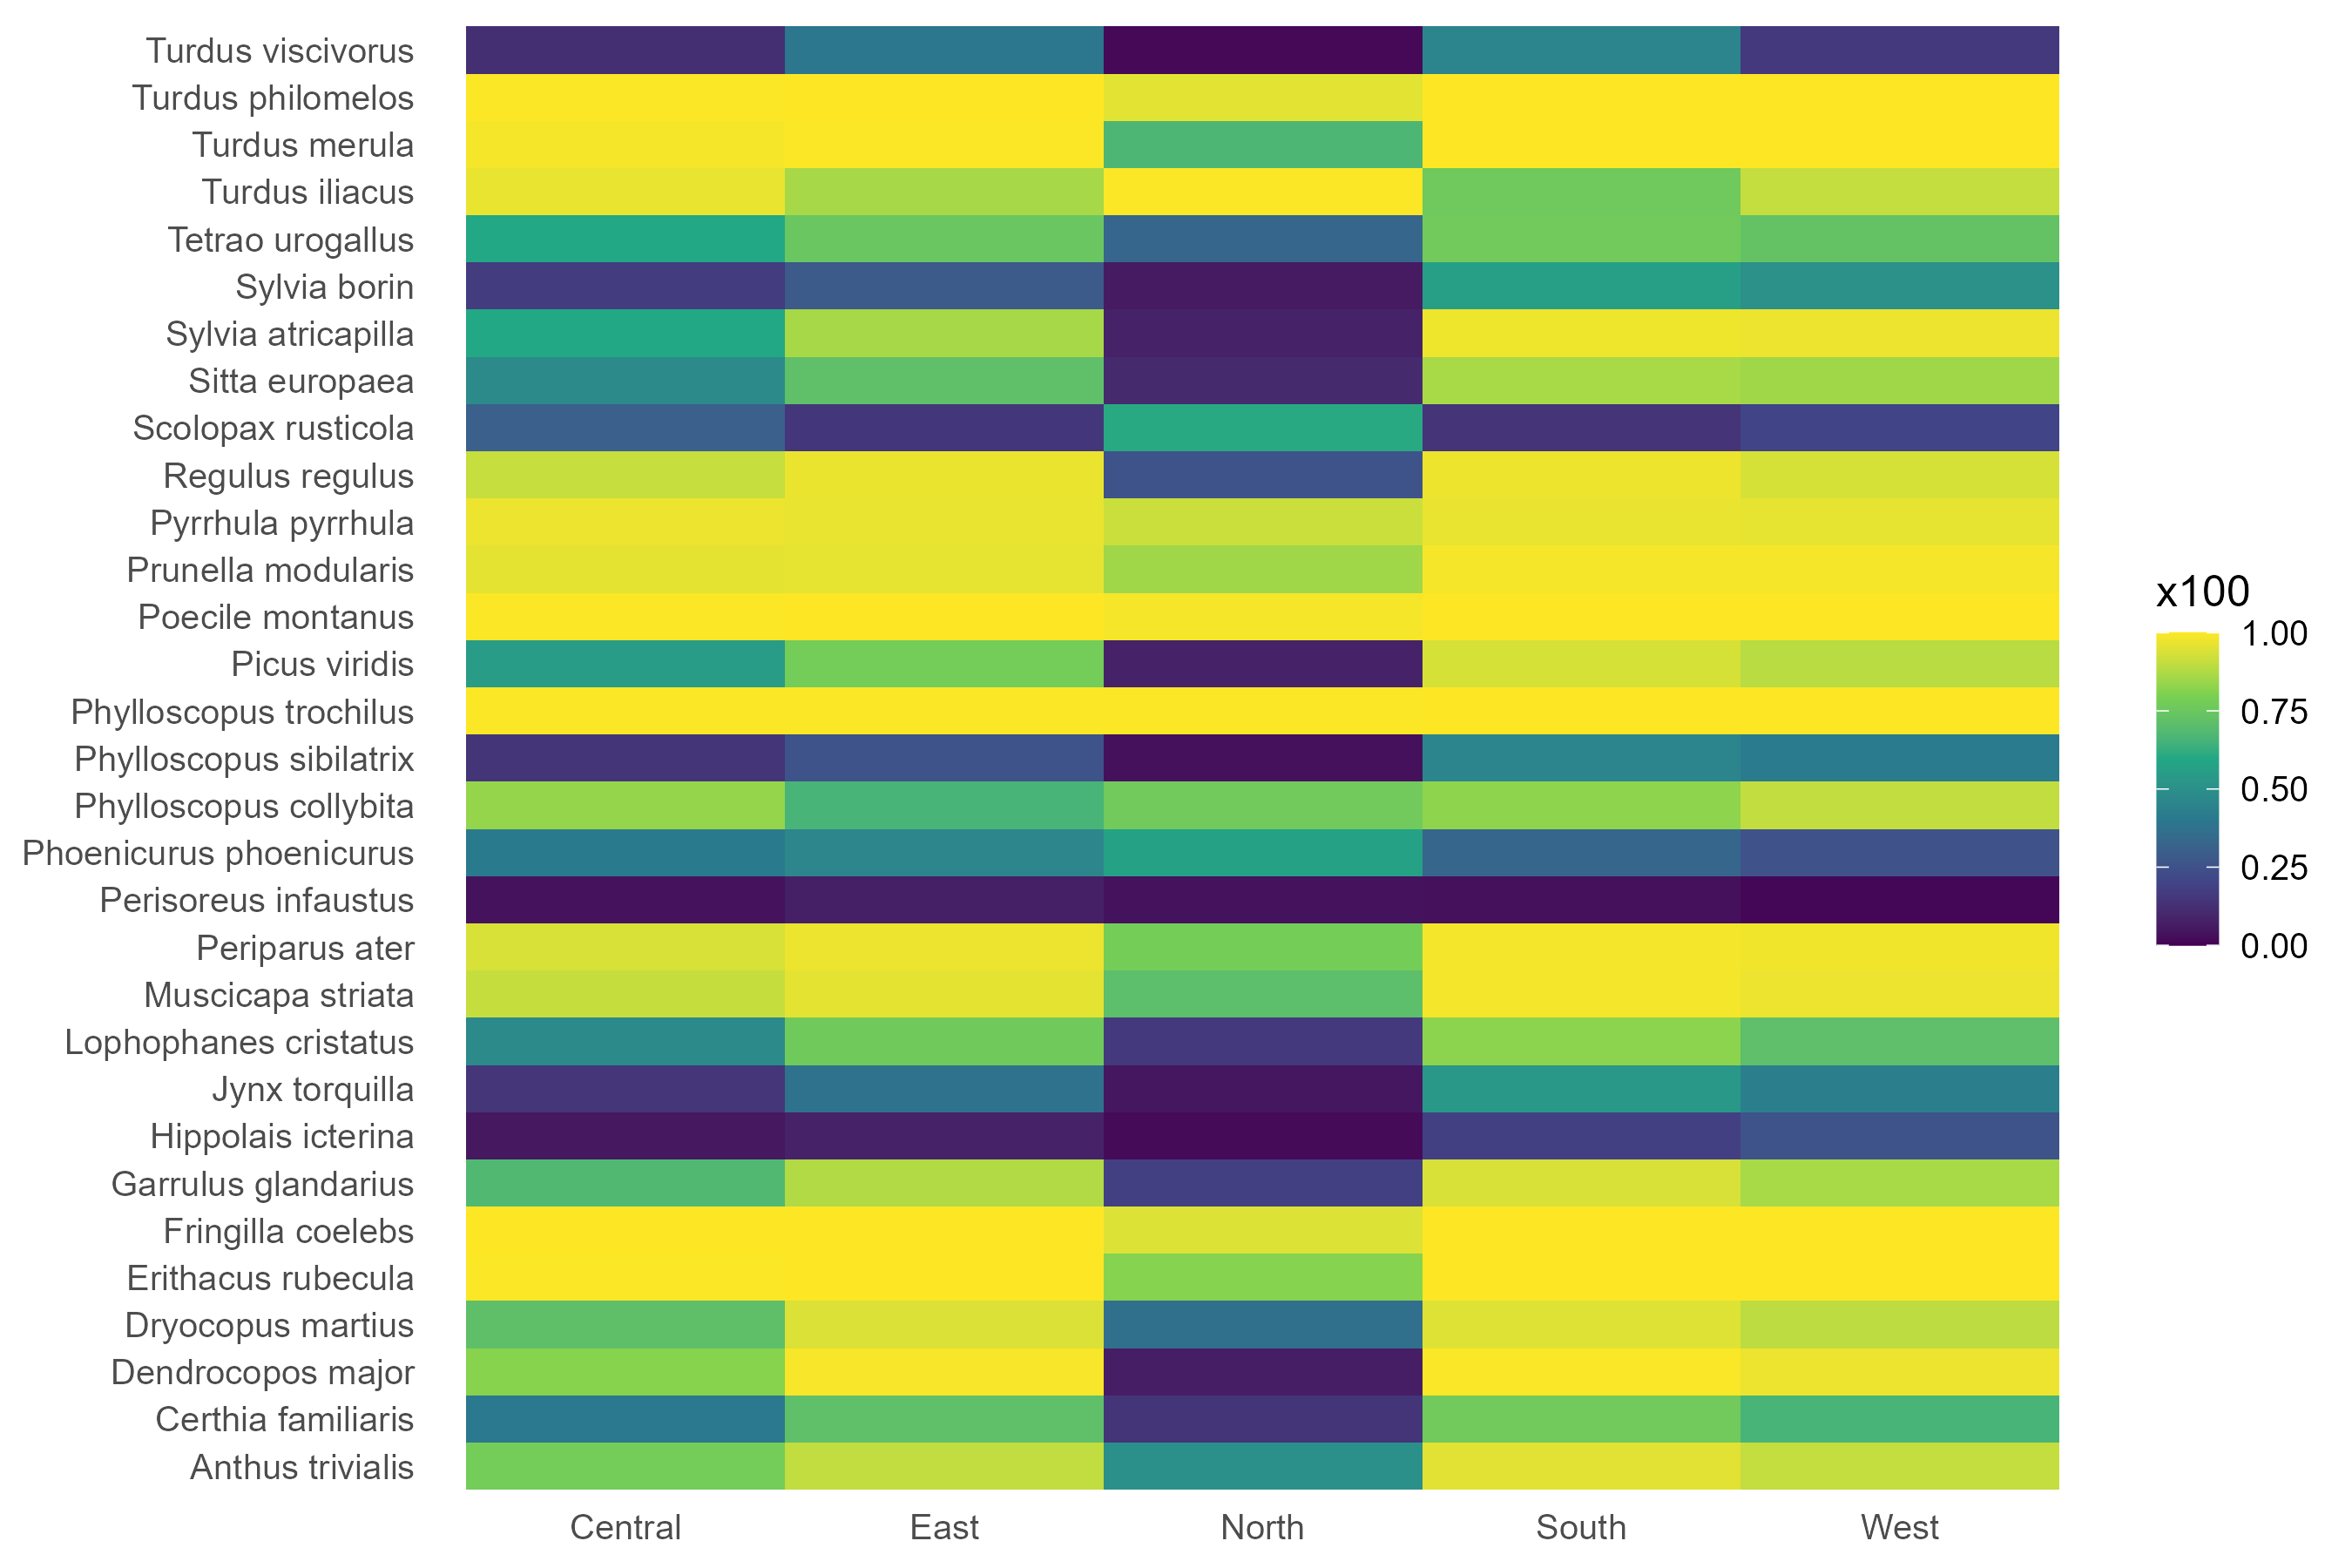
\includegraphics[width=1\linewidth,height=\textheight,keepaspectratio]{../img/forest/x100_reference_values.png}

}

\caption{\label{fig-forestX_100}Reference values (\(X_{100}\)) of each
characteristic forest species in each nature region. \(X_{100}\) is the
expert-assigned quantile of the species occupancy predicted within the
region, and ranges from 0 to 1. Species are rows and nature regions are
columns; yellow indicates values near 1 and dark purple values near 0.}

\end{figure}%

In mountain, four species (meadow pipit, European golden plover,
northern wheatear and rock ptarmigan \emph{Lagopus muta}; see
Figure~\ref{fig-MountainX100}) had reference values near \(1\) in all
regions. Lapland longspur \emph{Calcarius lapponicus} had values near
\(0\) in all regions except the North, and shore lark \emph{Eremophila
alpestris} and bluethroat \emph{Luscinia svecica} had low values in most
regions.

\begin{figure}

\centering{

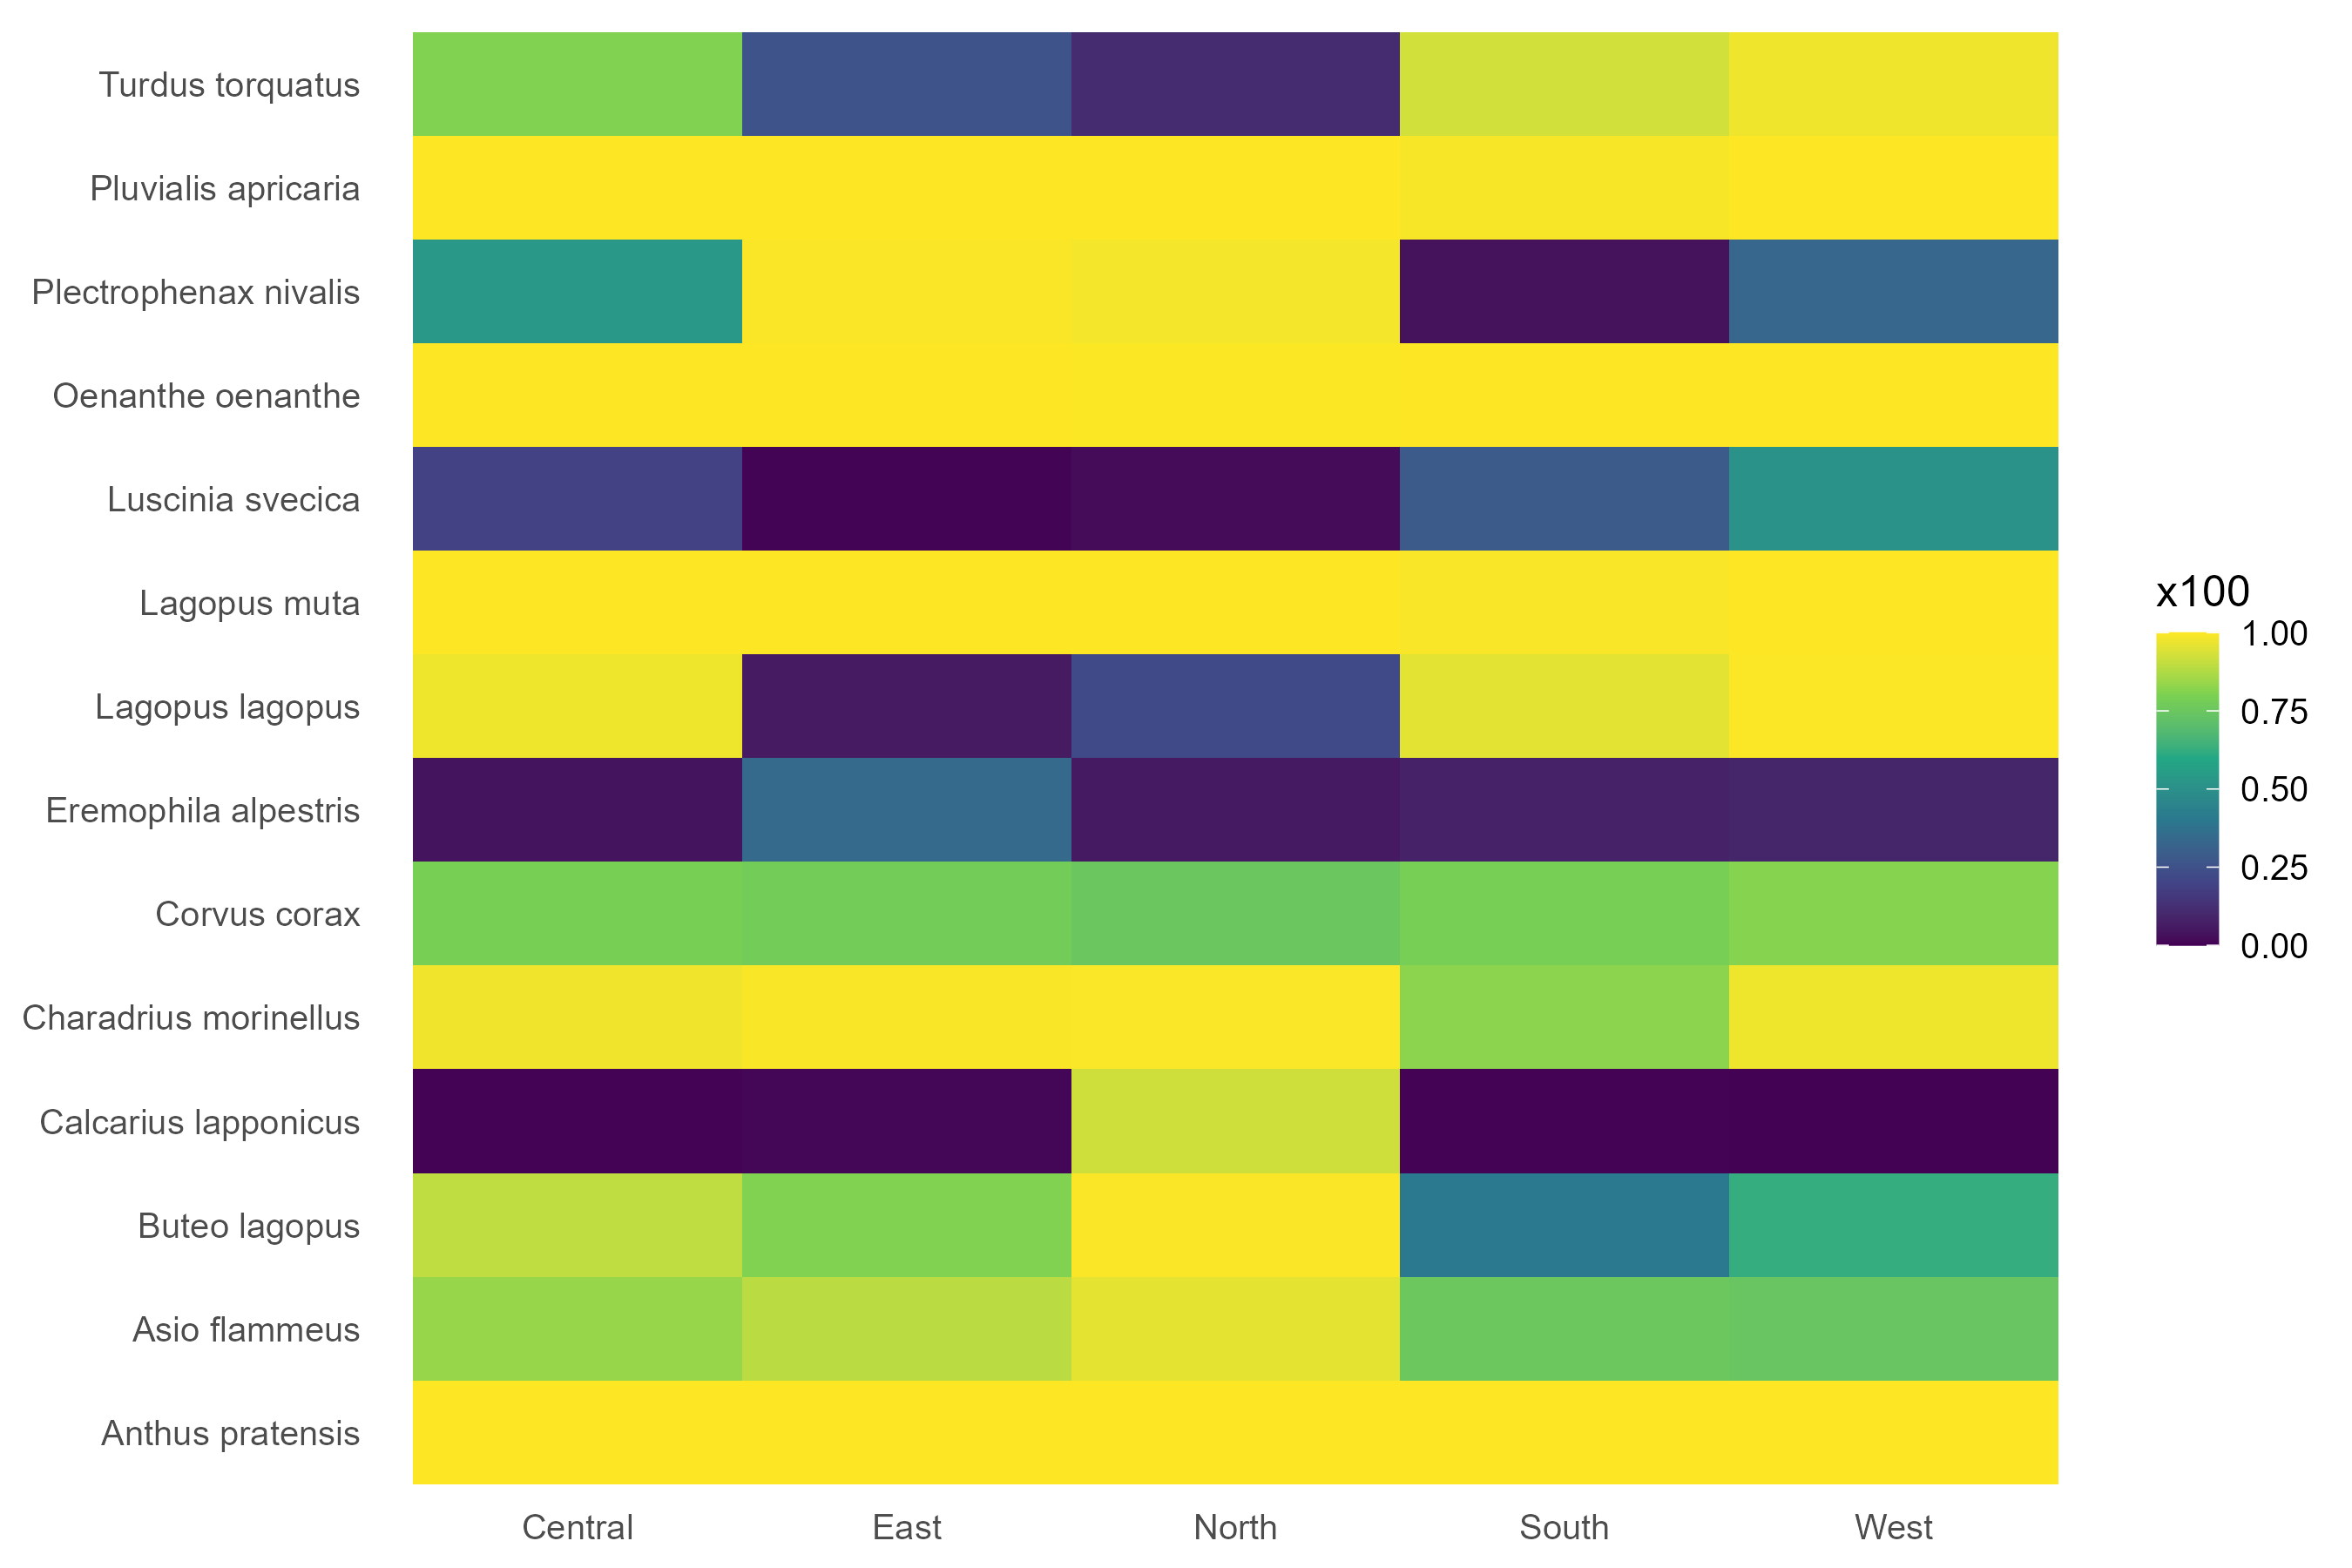
\includegraphics[width=1\linewidth,height=\textheight,keepaspectratio]{../img/mountain/x100_reference_values.png}

}

\caption{\label{fig-MountainX100}Reference values (\(X_{100}\)) of each
characteristic mountain species in each nature region. \(X_{100}\) is
the expert-assigned quantile of the species occupancy predicted within
the region, and ranges from 0 to 1. Species are rows and nature regions
are columns; yellow indicates values near 1 and dark purple values near
0.}

\end{figure}%

Reference values at or near \(1\) mean that a species only adds to the
indicator in the locations where its occupancy is clearly high. Species
with very low reference values have the opposite effect: they reach a
scaled value of \(1\) at almost any location and therefore add little
information about differences in condition.

Only species with an expert reference category contribute to the
indicator. In the figures above, 31 of the 32 forest species and 14 of
the 16 mountain species are shown (golden eagle \emph{Aquila chrysaetos}
is missing from both ecosystems, and common kestrel \emph{Falco
tinnunculus} from the mountain ecosystem).

\subsubsection{10.2 Scaled indicator}\label{sec-indicatorValues}

\paragraph{10.2.1 Regional values}\label{sec-regionalValues}

The indicator is the average, over species, of occupancy scaled against
the reference value, so \(1\) means that on average species occur at or
above their reference levels and \(0\) means a strong departure.
Nationally, the indicator was \(0.67\) for forest and \(0.59\) for
mountain (Table~\ref{tbl-representativeVals}).

In forest, values were highest in the South (\(0.74\)) and similar in
the West (\(0.69\)), East (\(0.69\)) and Central (\(0.67\)) regions. The
North had the lowest value (\(0.54\)), clearly separated from the other
regions. In mountain, regional differences were smaller. Values were
highest in the North (\(0.64\)) and East (\(0.64\)), intermediate in
Central (\(0.57\)), and lowest in the South (\(0.54\)) and West
(\(0.53\)). Forest and mountain values should not be compared directly,
because the two indicators use different species lists and different
reference values.

The 95\% bootstrap intervals in Table~\ref{tbl-representativeVals} are
very narrow (about \(\pm 0.002\) to \(\pm 0.004\)). They only reflect
resampling of prediction locations. They do not include the uncertainty
in the occupancy predictions or the spatial dependence between nearby
locations (see Section~\ref{sec-uncertainties}), and should not be used
to judge whether two regions differ. Differences of a few hundredths,
such as West versus East in forest or North versus East in mountain,
should be regarded as negligible.

\begin{table}

\caption{\label{tbl-representativeVals}Regional and national estimates
of the breeding bird indicator for the forest and mountain ecosystems.
Values are the mean and the 2.5\% (Lower) and 97.5\% (Upper) quantiles
of the bootstrap estimates. Regional estimates come from intercept-only
beta regressions and the national estimate from a beta mixed model with
nature region as a random effect. The indicator ranges from 0 to 1,
where 1 means that, on average, species occupancy is at or above the
reference values. The intervals reflect resampling of prediction
locations only.}

\centering{

\begin{xltabular}{\linewidth}{>{\raggedright\arraybackslash}X>{\raggedright\arraybackslash}X>{\raggedleft\arraybackslash}X>{\raggedleft\arraybackslash}X>{\raggedleft\arraybackslash}X}
\toprule
Ecosystem type & Region & Mean & Lower & Upper\\
\midrule
Forest & National & 0.668 & 0.666 & 0.670\\
Forest & Central & 0.670 & 0.666 & 0.674\\
Forest & East & 0.686 & 0.681 & 0.690\\
Forest & North & 0.538 & 0.533 & 0.543\\
Forest & South & 0.744 & 0.740 & 0.748\\
\addlinespace
Forest & West & 0.693 & 0.689 & 0.697\\
Mountain & National & 0.585 & 0.584 & 0.586\\
Mountain & Central & 0.574 & 0.571 & 0.576\\
Mountain & East & 0.639 & 0.637 & 0.641\\
Mountain & North & 0.643 & 0.641 & 0.645\\
\addlinespace
Mountain & South & 0.539 & 0.537 & 0.542\\
Mountain & West & 0.528 & 0.525 & 0.532\\
\bottomrule
\end{xltabular}

}

\end{table}%

\paragraph{10.2.2 Sensitivity to the reference
quantile}\label{sec-sensitivity}

The quantile linked to the expert category \emph{samme} (same) and
\emph{høyere} (higher) is a subjective choice, so we tested quantiles
from \(0.5\) to \(0.9\) for the expert category \emph{samme} (the main
results use \(0.75\)) keeping that of \emph{høyere} fixed. Raising the
quantile raises the reference values and lowers the indicator in all
regions (Figure~\ref{fig-forestSensitivity},
Figure~\ref{fig-mountainSensitivity}). Nationally, the forest indicator
decreased from about \(0.72\) to \(0.63\) and the mountain indicator
from about \(0.65\) to \(0.55\). The decline was steepest in the forest
North region (from about \(0.62\) to \(0.47\)).

\begin{figure}

\begin{minipage}[t]{\linewidth}

\centering{

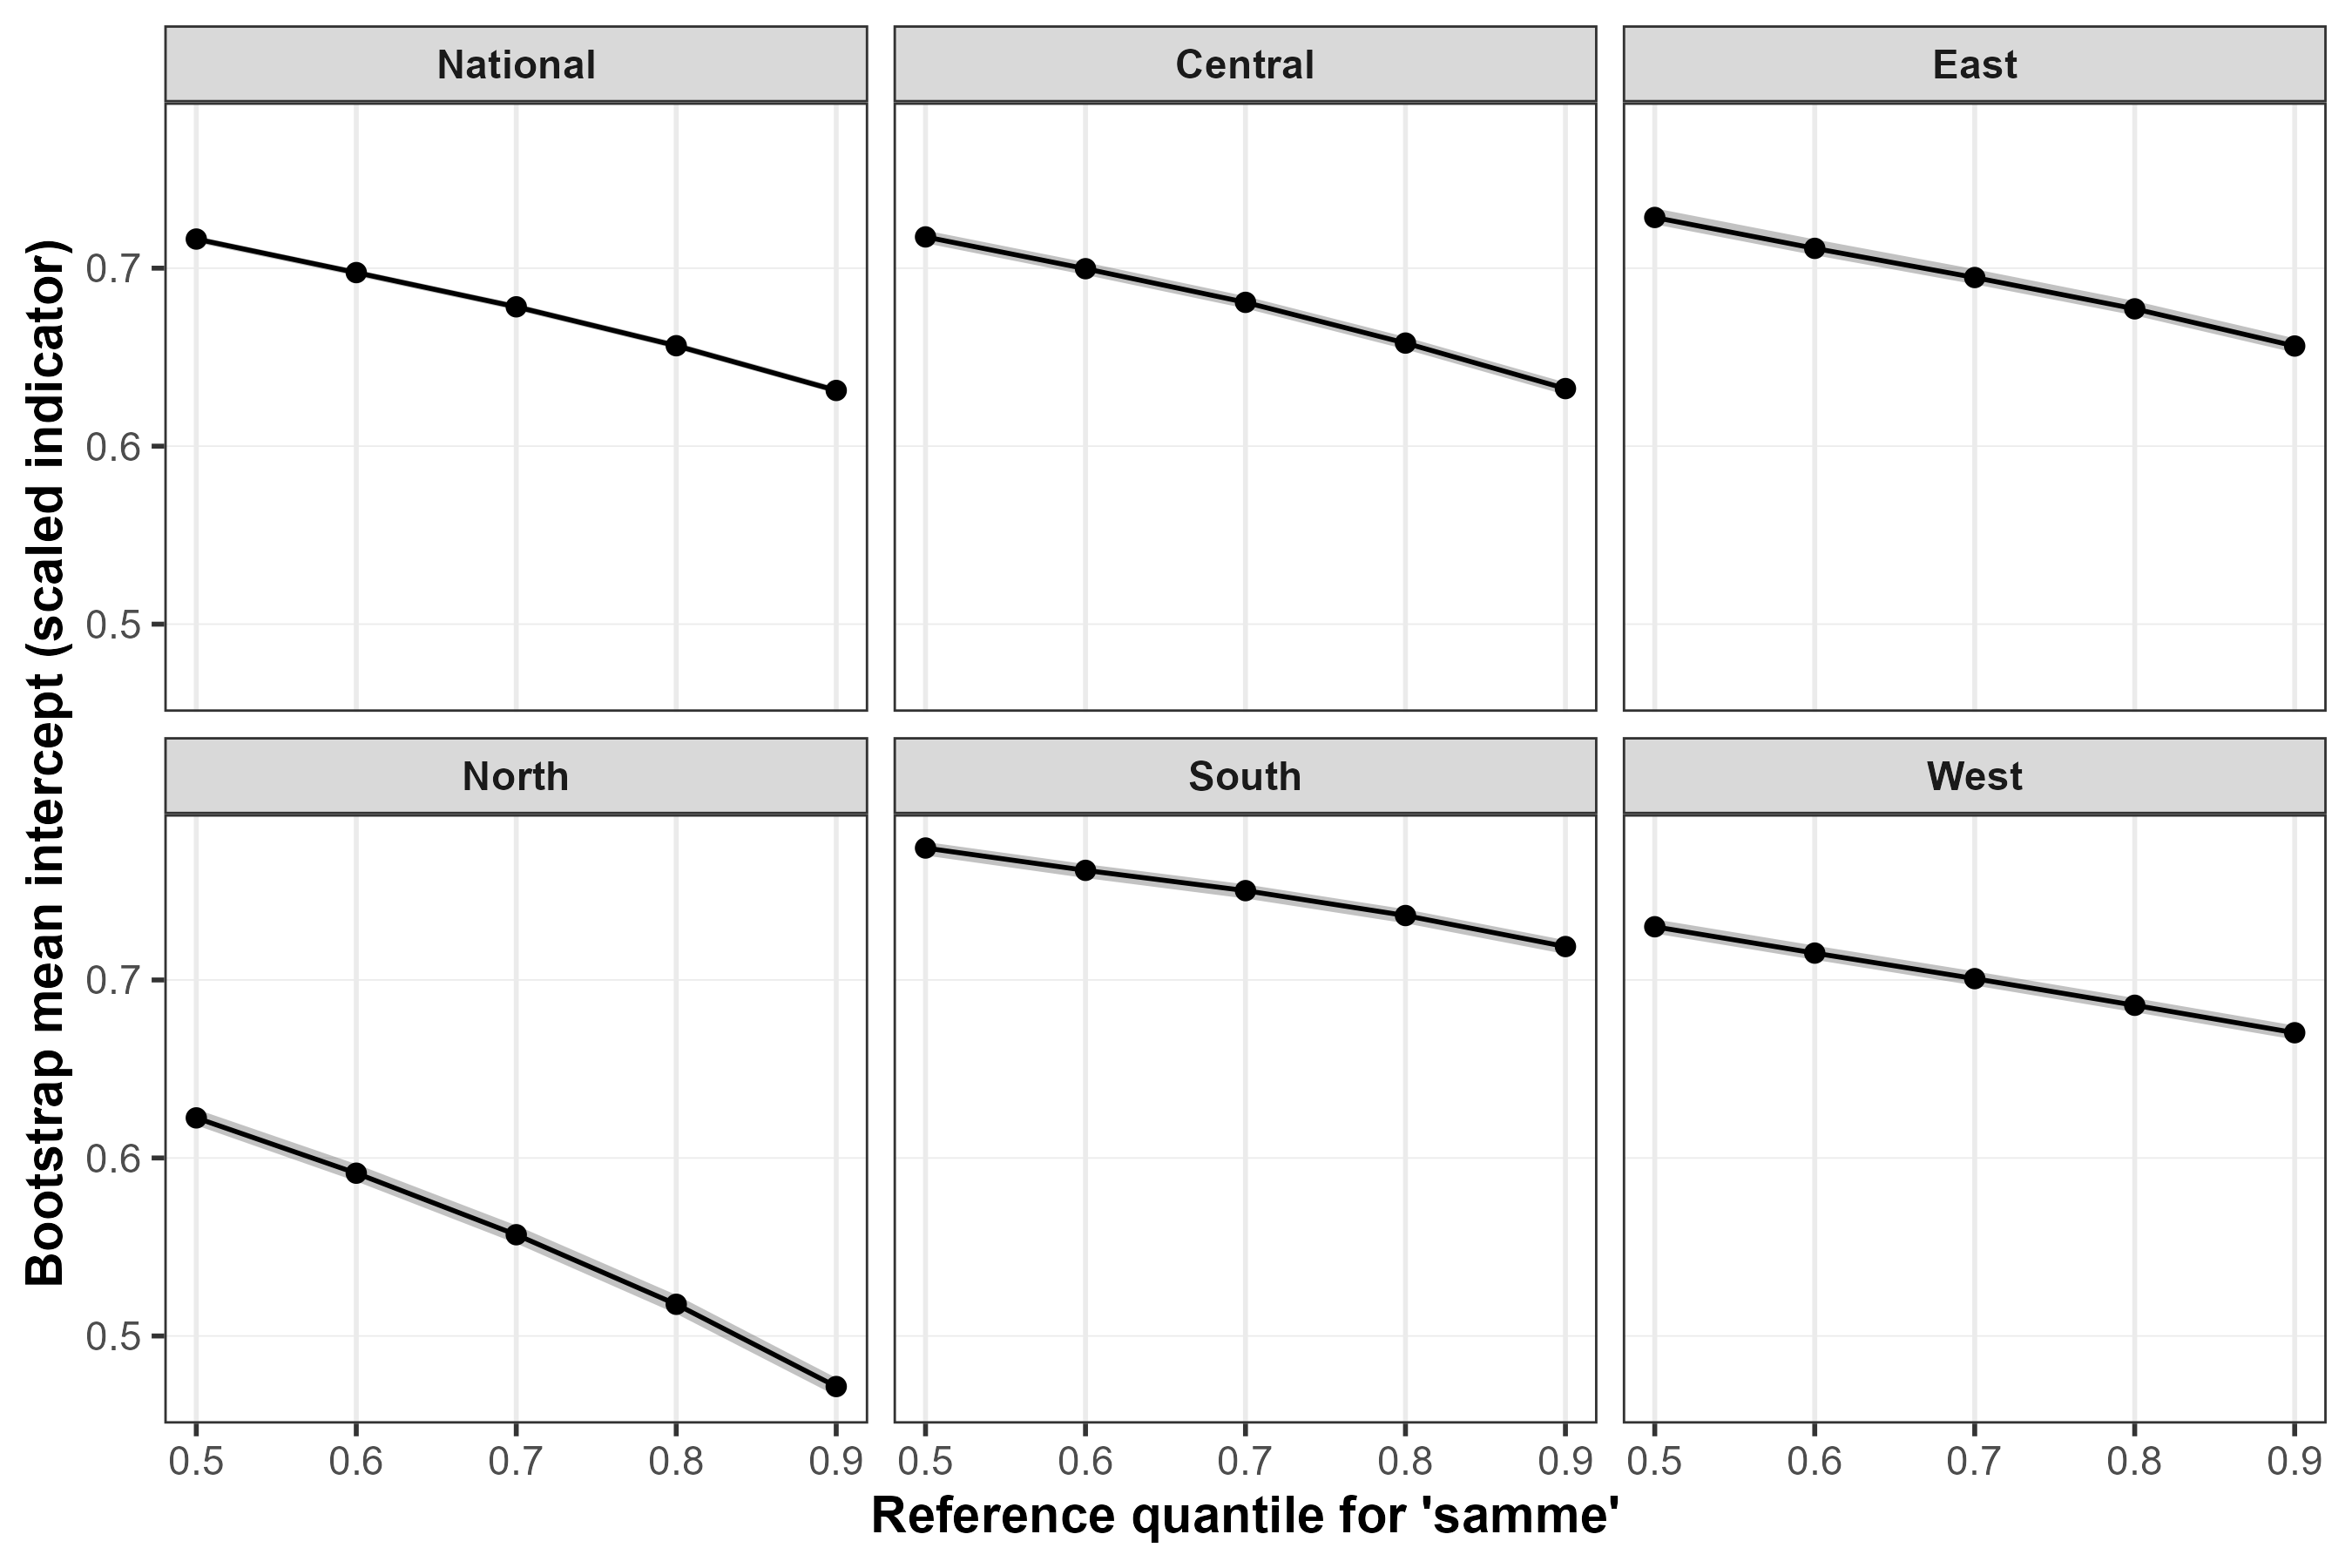
\includegraphics[width=1\linewidth,height=\textheight,keepaspectratio]{../img/forest/indicator_estimate_vs_samme_quantile.png}

}

\subcaption{\label{fig-forestSensitivity-1}Indicator estimate and 95\%
bootstrap interval for each nature region and nationally, by
\emph{samme} quantile.}

\end{minipage}%
\newline
\begin{minipage}[t]{\linewidth}

\centering{

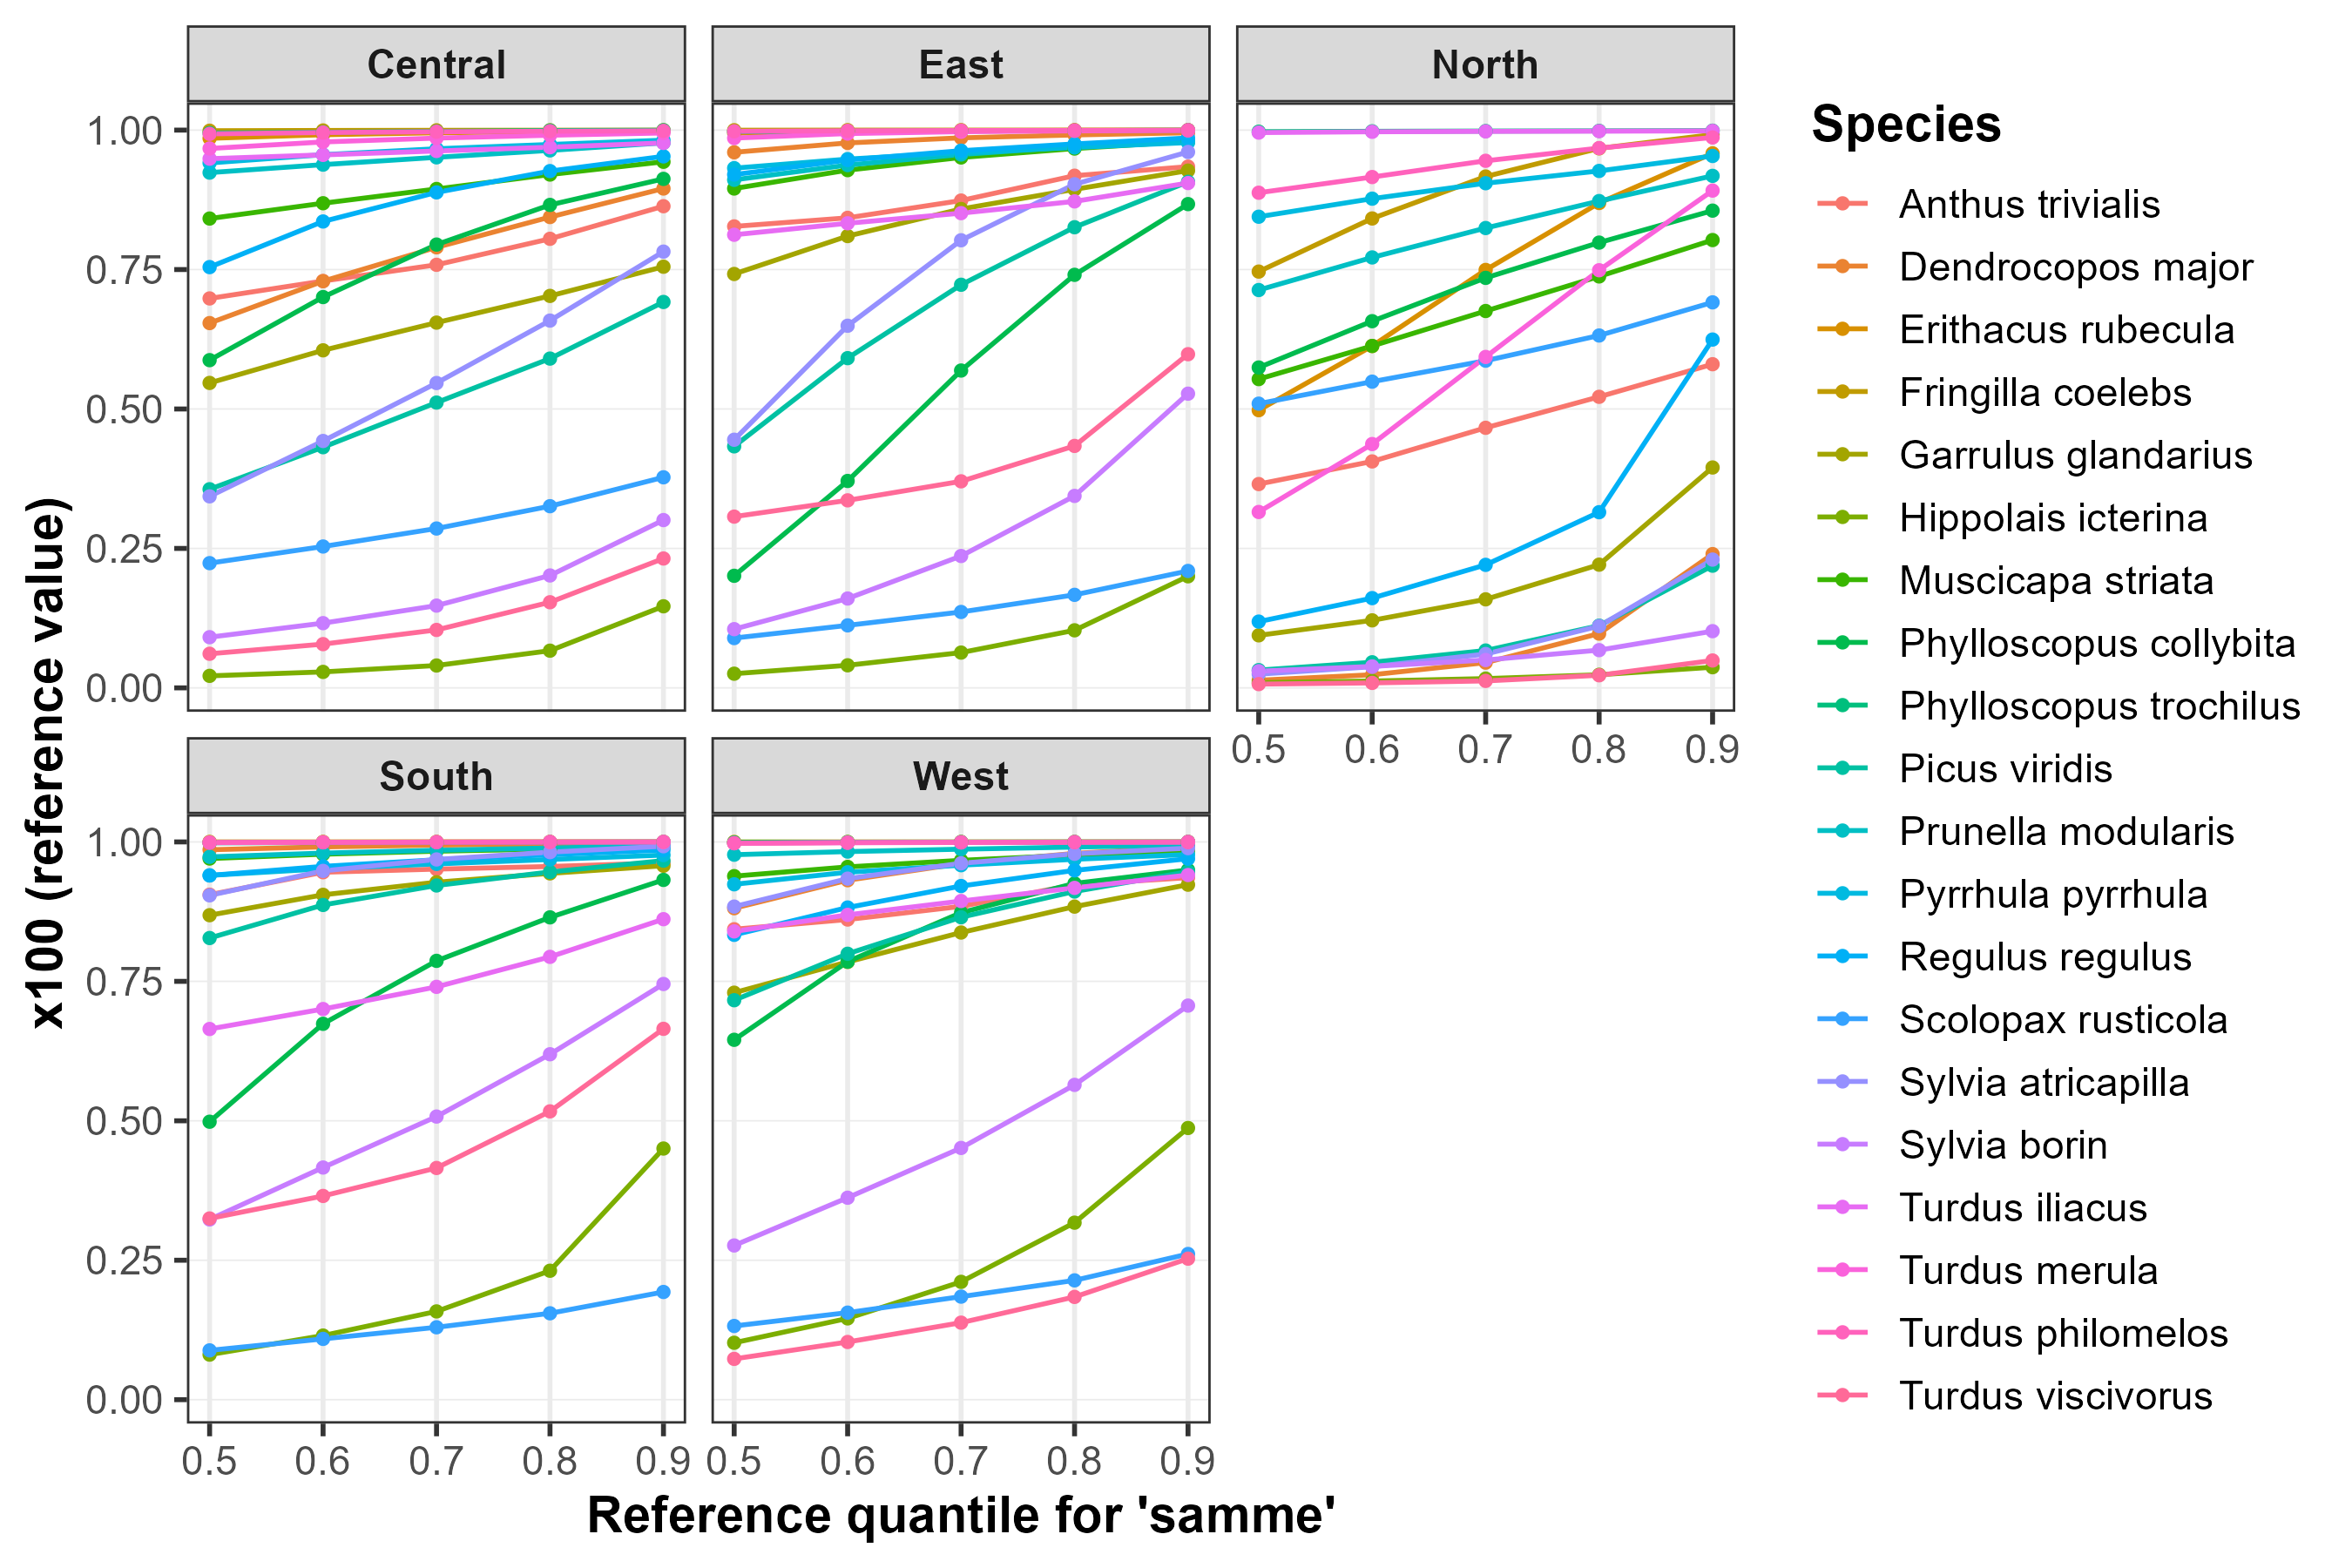
\includegraphics[width=1\linewidth,height=\textheight,keepaspectratio]{../img/forest/x100_vs_samme_quantile_by_species.png}

}

\subcaption{\label{fig-forestSensitivity-2}Reference value (\(x_{100}\))
of each species in the \emph{samme} category, by quantile. Species whose
reference value is already close to 1 change little, whereas species
with low occupancy over most of a region change most.}

\end{minipage}%

\caption{\label{fig-forestSensitivity}Sensitivity of the forest breeding
bird indicator to the quantile linked to the expert category
\emph{samme}. The quantile was varied from 0.5 to 0.9, while the
\emph{høyere} quantile was kept at 0.95. The same bootstrap seed was
used for every quantile, so differences reflect the quantile and not
bootstrap noise.}

\end{figure}%

The ordering of regions was largely stable: the forest North region
remained the lowest at all quantiles, and in mountain the North and East
regions remained at the top, and the South and West regions at the
bottom. Some regions that differ little in the main results, such as the
mountain North and East, and the mountain South and West, became
practically identical at a quantile of \(0.9\). The absolute indicator
values therefore depend on the reference choice, whereas the main
regional contrasts do not. The sensitivity analysis used fewer bootstrap
replicates and a smaller sample per region than the main analysis
(\(100\) replicates and \(5\,000\) values), which does not affect the
conclusion because the same bootstrap seed was used for every quantile.

\begin{figure}

\begin{minipage}[t]{\linewidth}

\centering{

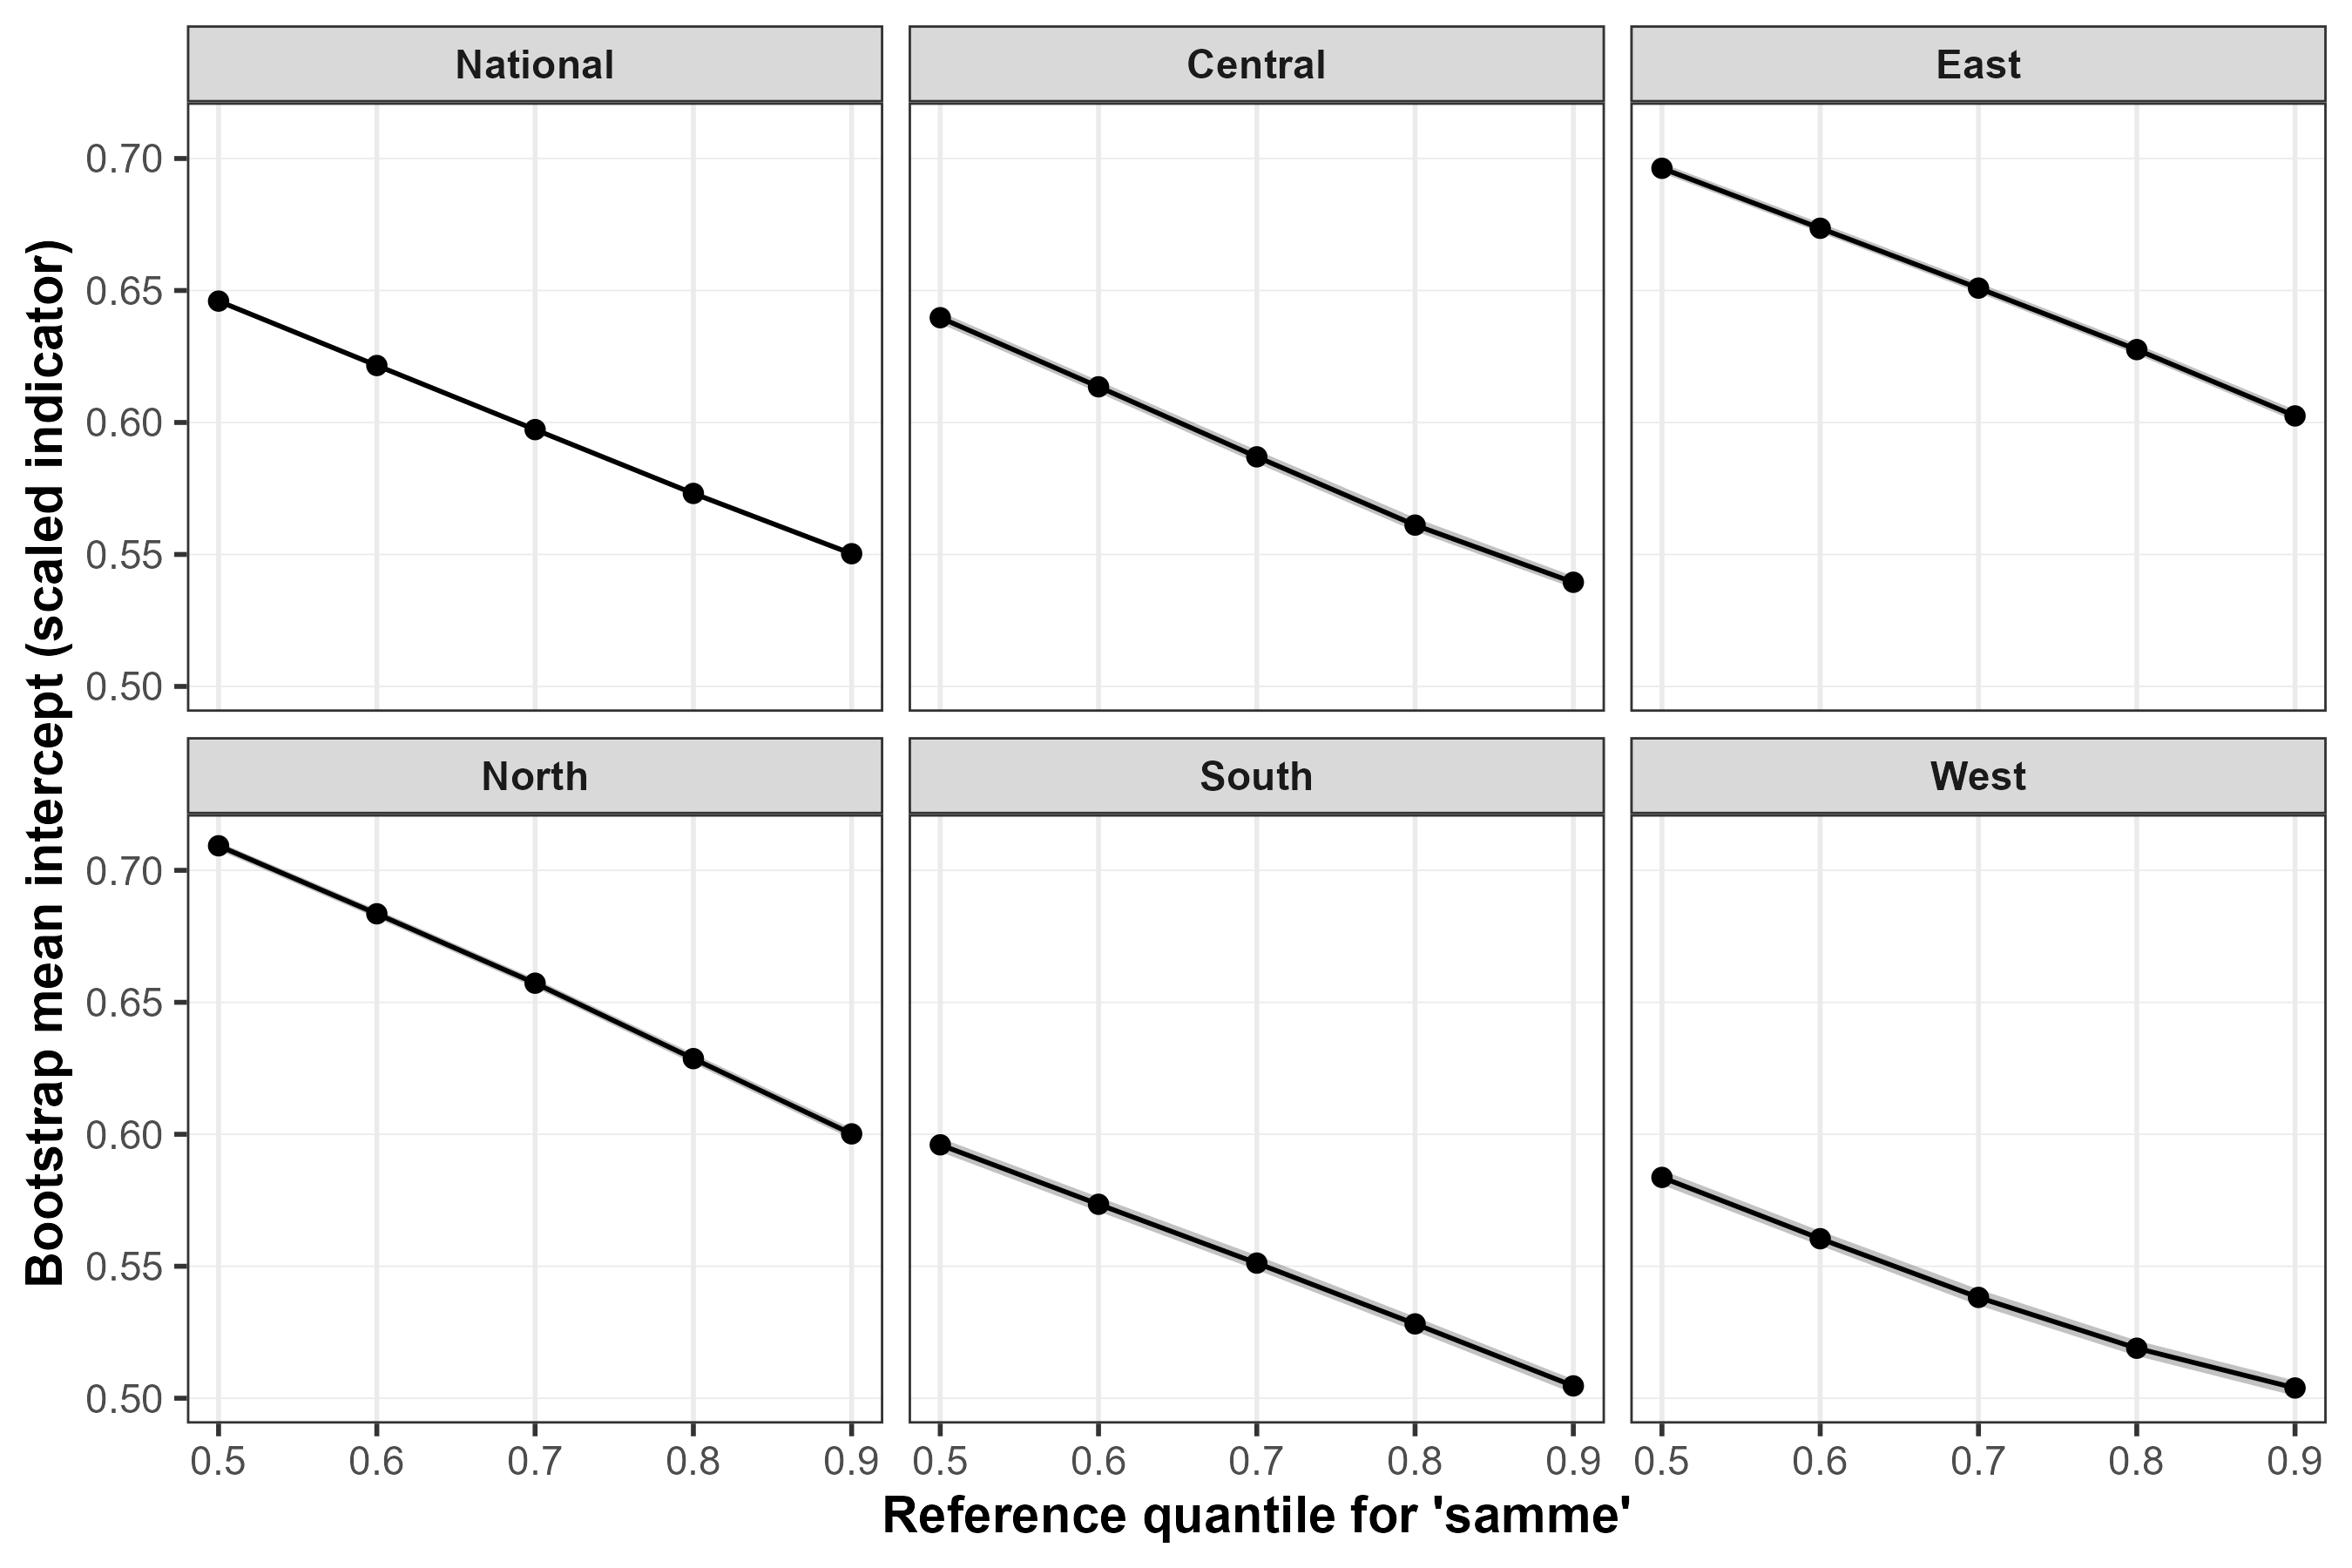
\includegraphics[width=1\linewidth,height=\textheight,keepaspectratio]{../img/mountain/indicator_estimate_vs_samme_quantile.png}

}

\subcaption{\label{fig-mountainSensitivity-1}Indicator estimate and 95\%
bootstrap interval for each nature region and nationally, by
\emph{samme} quantile.}

\end{minipage}%
\newline
\begin{minipage}[t]{\linewidth}

\centering{

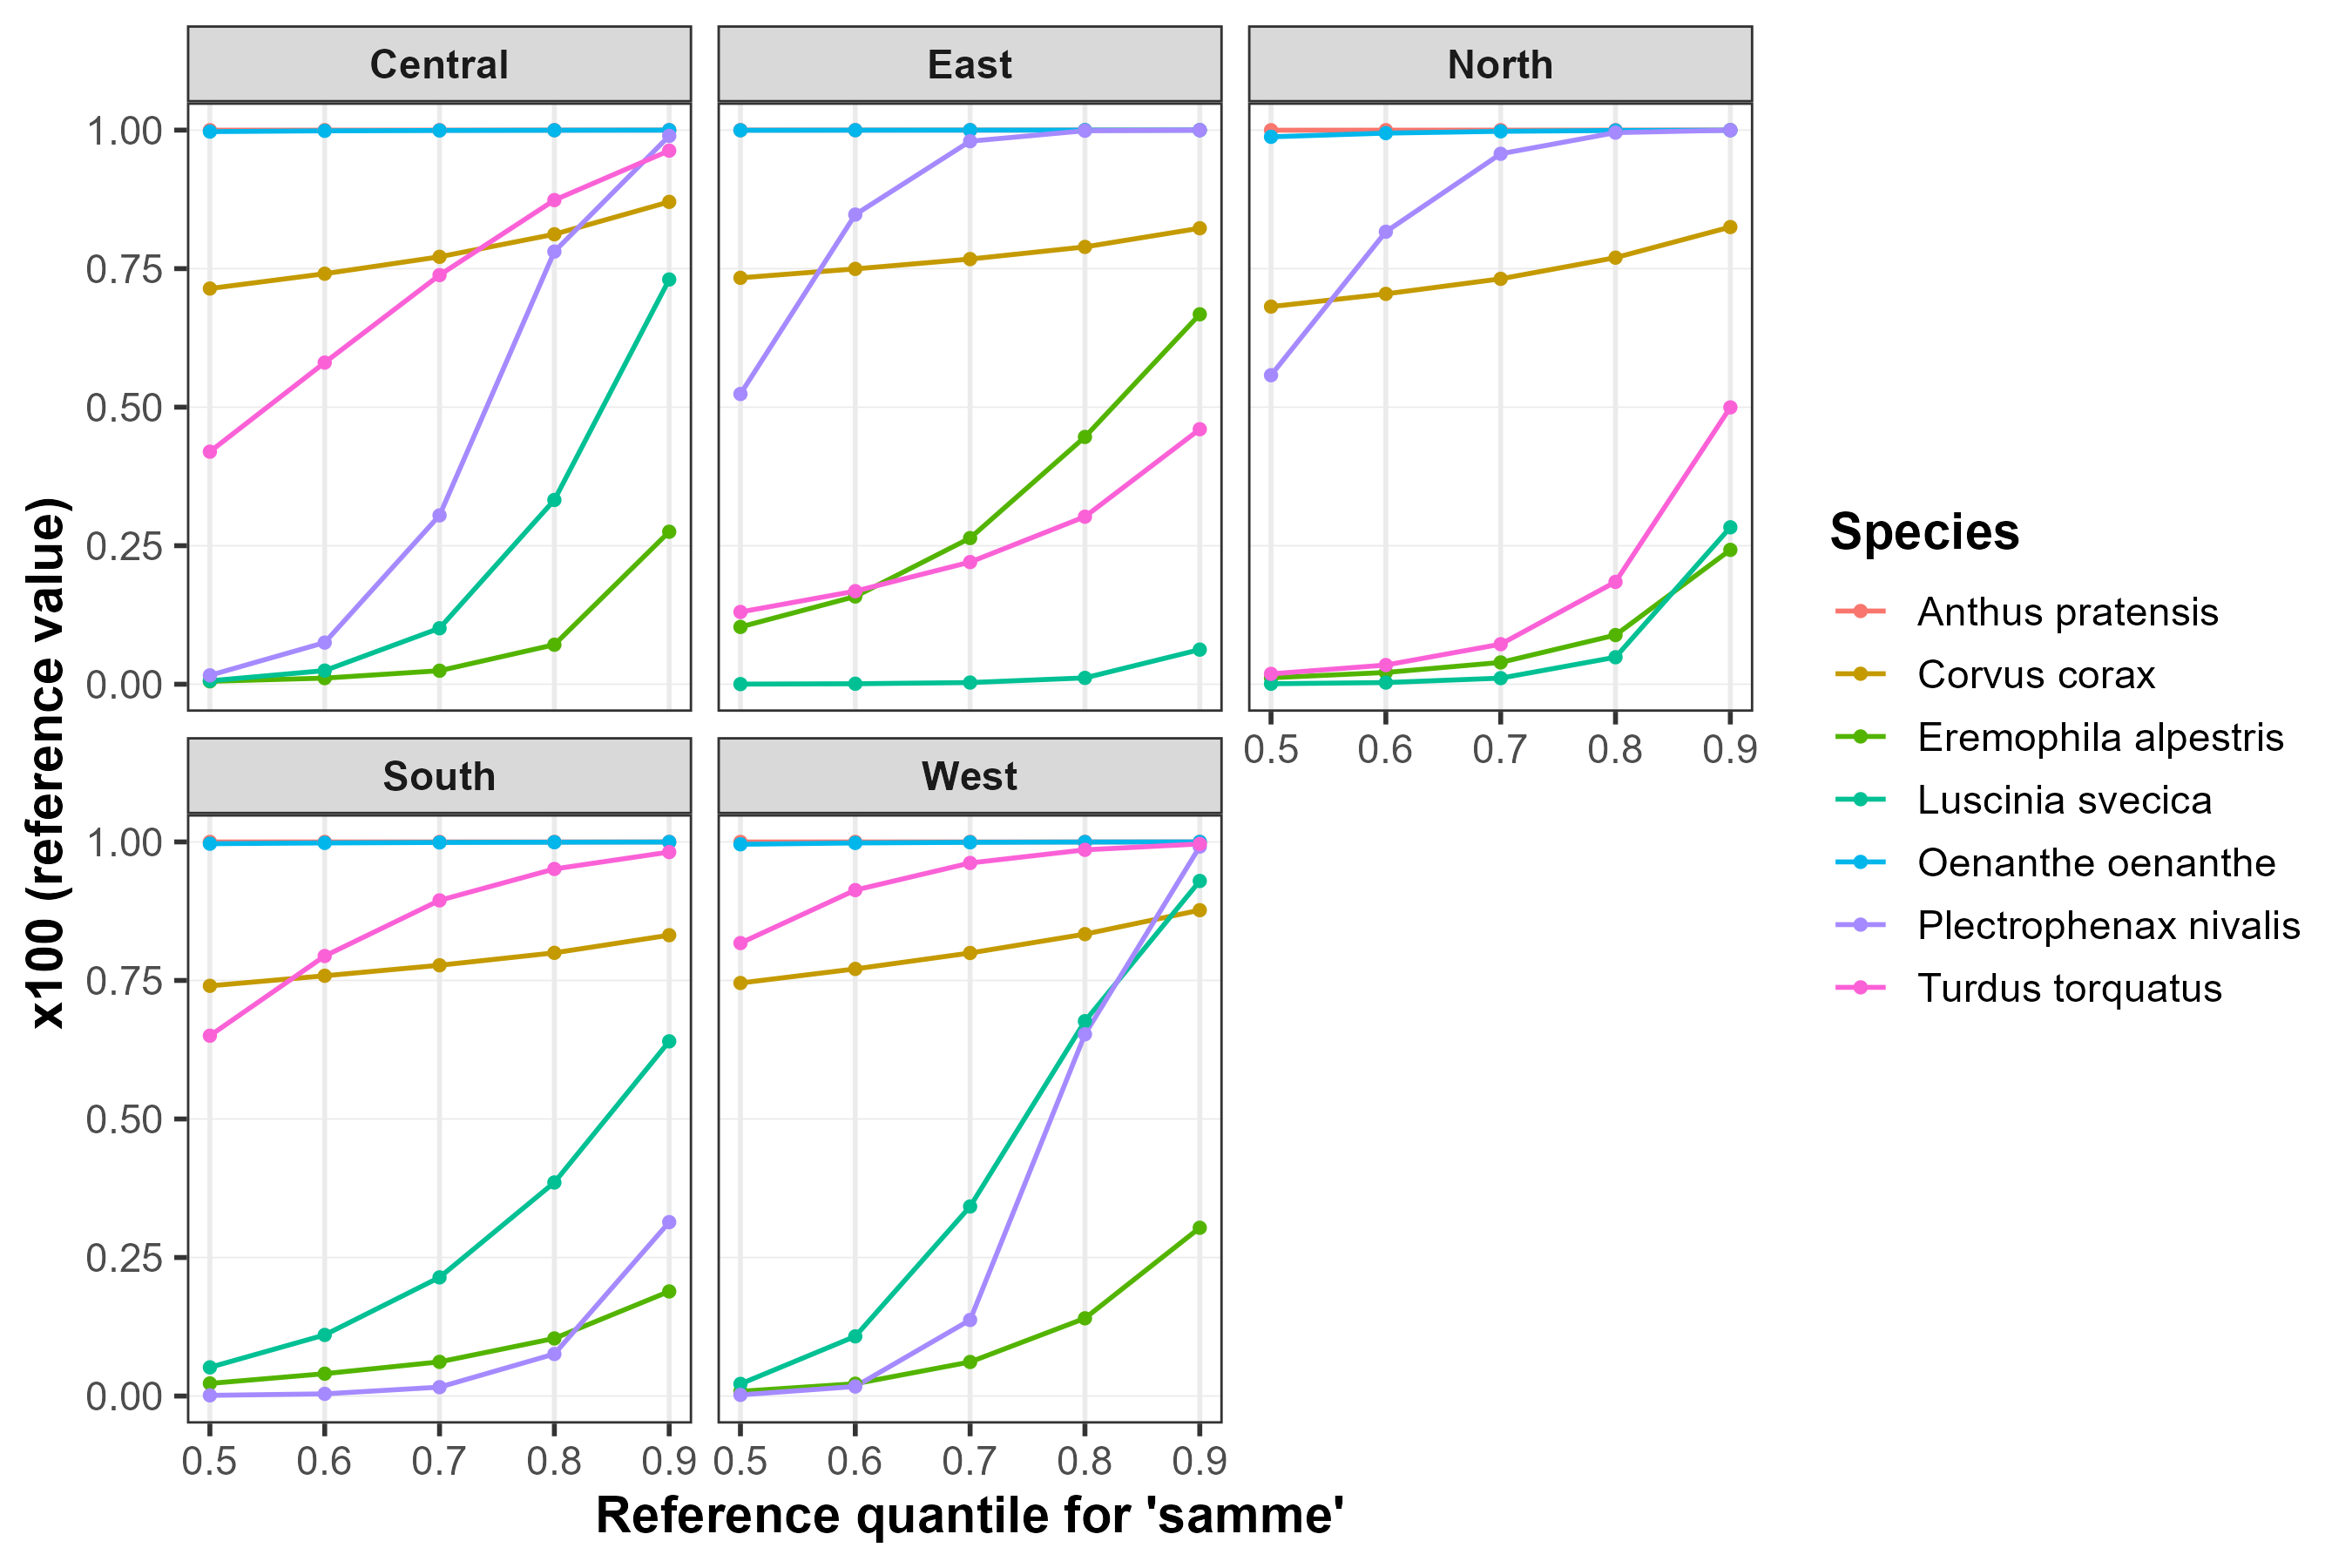
\includegraphics[width=1\linewidth,height=\textheight,keepaspectratio]{../img/mountain/x100_vs_samme_quantile_by_species.png}

}

\subcaption{\label{fig-mountainSensitivity-2}Reference value
(\(x_{100}\)) of each species in the \emph{samme} category, by quantile.
Species whose reference value is already close to 1 change little,
whereas species with low occupancy over most of a region change most.}

\end{minipage}%

\caption{\label{fig-mountainSensitivity}Sensitivity of the mountain
breeding bird indicator to the quantile linked to the expert category
\emph{samme}. The quantile was varied from 0.5 to 0.9, while the
\emph{høyere} quantile was kept at 0.95. The same bootstrap seed was
used for every quantile, so differences reflect the quantile and not
bootstrap noise.}

\end{figure}%

Species that already had reference values close to \(1\) changed very
little, whereas species with low occupancy in most of a region changed
most (second panel of each figure).

\paragraph{10.2.3 Relationship between the indicator and environmental
variables}\label{sec-covariates}

Figure~\ref{fig-forestScaledIndicatorVrsCovs} and
Figure~\ref{fig-mountainScaledIndicatorVrsCovs} show how the indicator
varies with the environmental variables at the prediction locations.
These plots are descriptive. The variables are the same ones that were
used to predict occupancy, so the plots show how the model translates
environment into the indicator, not independent evidence of what drives
condition.

\begin{figure}

\centering{

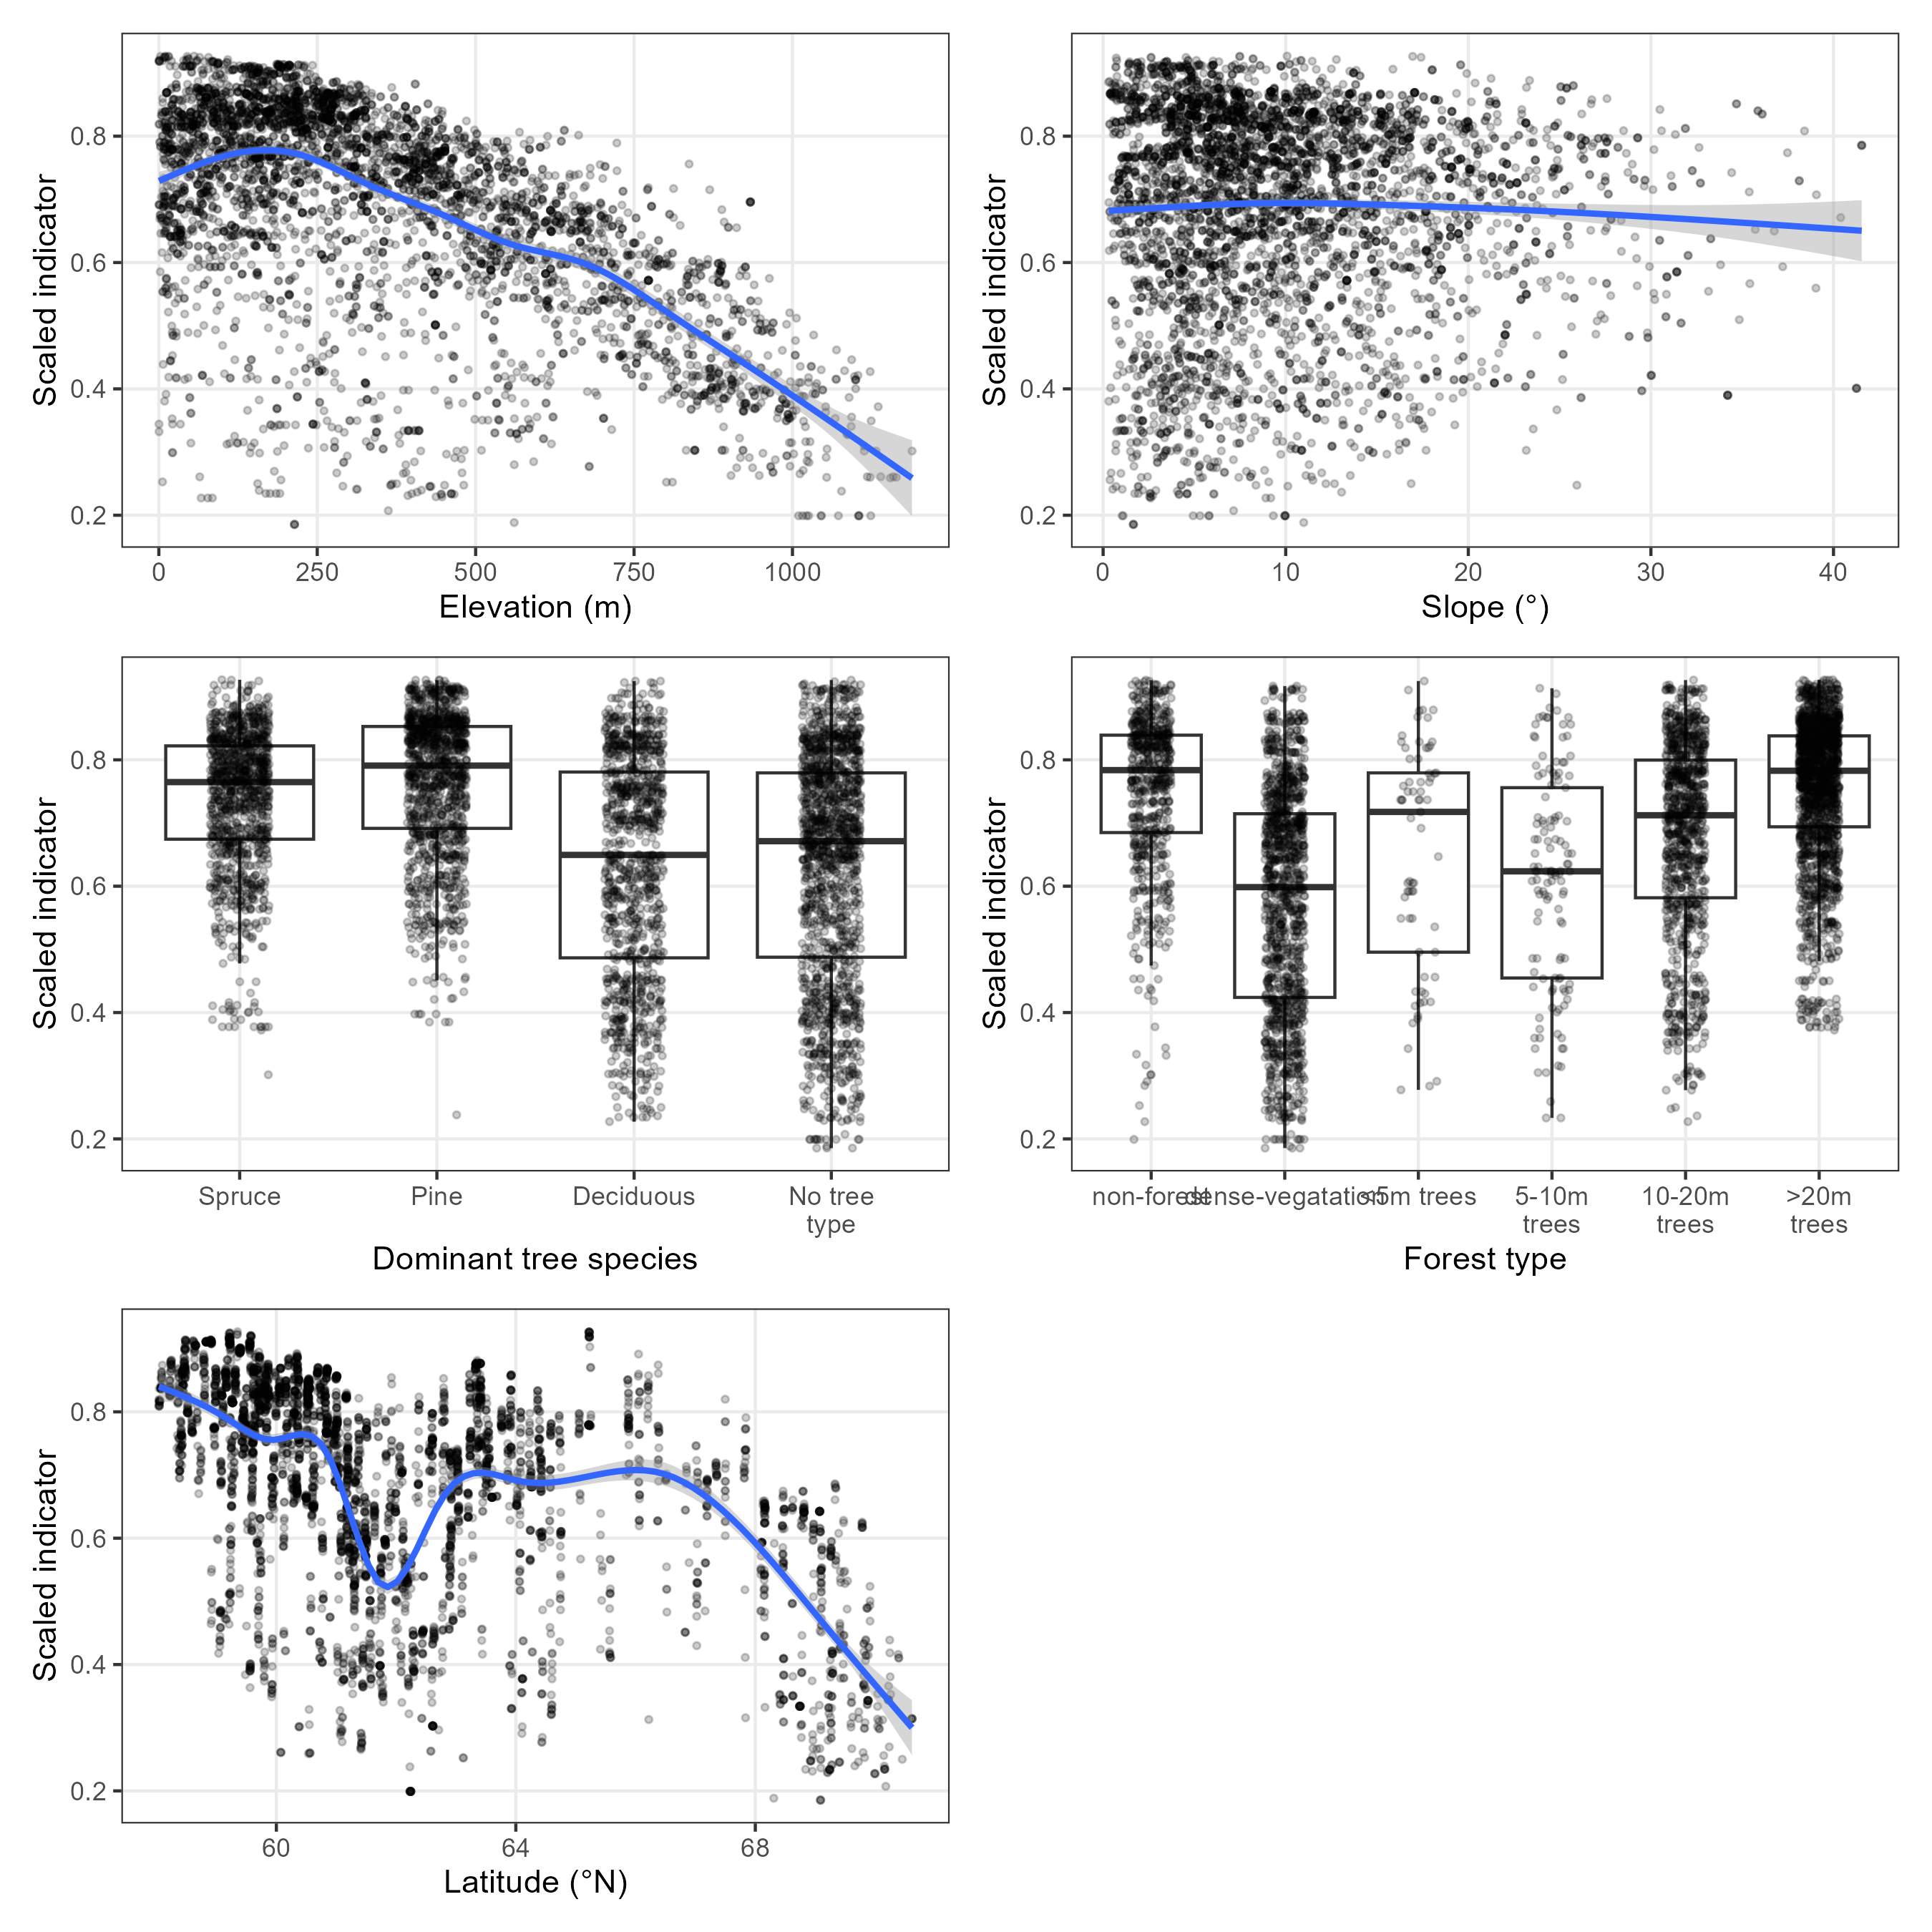
\includegraphics[width=1\linewidth,height=\textheight,keepaspectratio]{../img/forest/model_indicator_vs_covariates.png}

}

\caption{\label{fig-forestScaledIndicatorVrsCovs}Predicted scaled
indicator for forest ecosystems in relation to elevation, slope,
dominant tree species, forest type and latitude. Each point is a
prediction location. Blue lines show smoothed trends, with shaded bands
indicating their uncertainty; boxplots summarise categorical variables.}

\end{figure}%

In forest, the indicator declined with increasing elevation (from about
\(0.75\)--\(0.80\) below \(250\) m to about \(0.3\) near \(1\,000\) m or
higher) and towards the north, with a pronounced dip around
\(62^{\circ}\)N and a steep decline north of about \(68^{\circ}\)N.
There was little association with slope. The indicator was higher in
spruce- and pine-dominated forest than in deciduous or non-forest-typed
locations, and higher in tall forest (\(>20\) m) than in dense
vegetation or low forest (\(<5\) m and \(5\)--\(10\) m).

\begin{figure}

\centering{

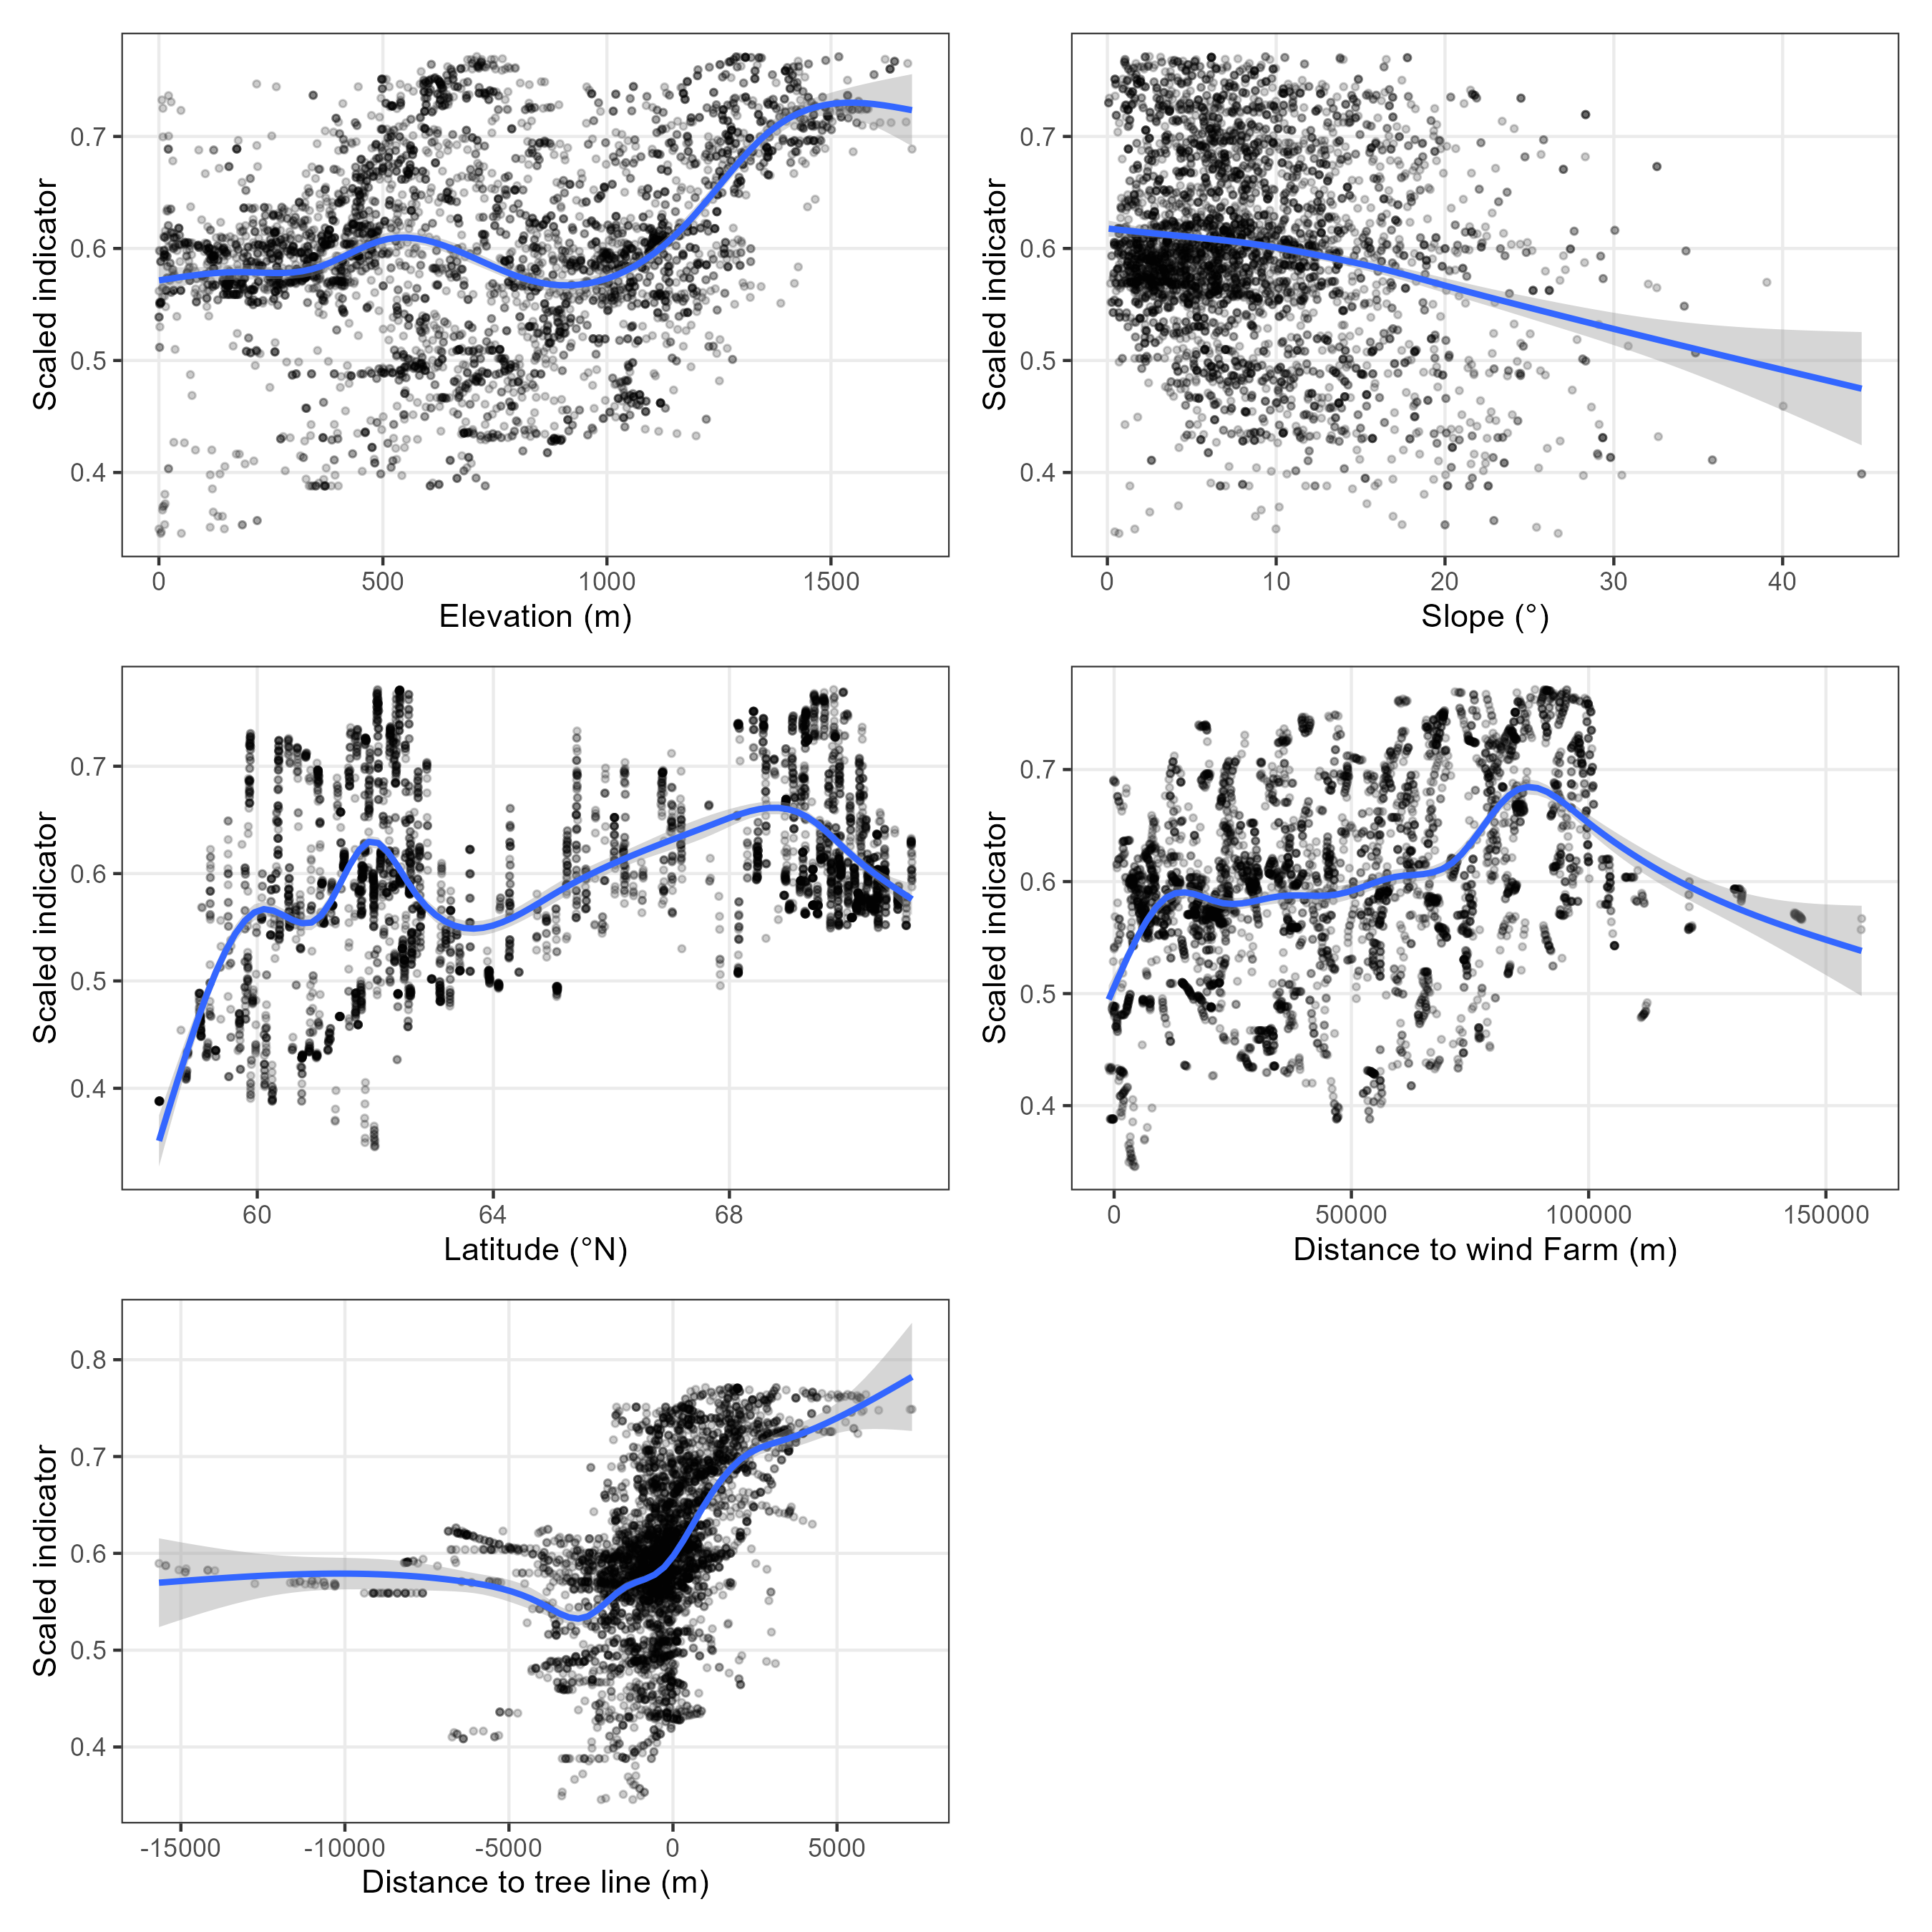
\includegraphics[width=1\linewidth,height=\textheight,keepaspectratio]{../img/mountain/model_indicator_vs_covariates.png}

}

\caption{\label{fig-mountainScaledIndicatorVrsCovs}Predicted scaled
indicator for mountain ecosystems in relation to elevation, slope,
latitude, distance to the nearest wind farm and distance to the tree
line (negative values are below the tree line). Each point is a
prediction location. Blue lines show smoothed trends, with shaded bands
indicating their uncertainty.}

\end{figure}%

In mountain, the indicator was higher above about \(1\,200\) m and above
the tree line, and it declined modestly with increasing slope. The
patterns with latitude and distance to the nearest wind farm were
irregular. The distance-to-wind-farm pattern should not be interpreted
as an effect of wind power, because wind farms are clustered
geographically and distance to a wind farm is confounded with location
and elevation.

The strong decline of the forest indicator with elevation and latitude
likely reflects, at least in part, natural limits on the occurrence of
forest bird species rather than reduced condition. The reference values
are set within regions and do not fully remove these gradients (see
Section~\ref{sec-uncertainties}).

\subsubsection{10.3 Effects of covariates on occupancy and
detection}\label{sec-effects}

Species-specific coefficients show how each covariate relates to
occupancy and detection in the multi-species spatial models.
Coefficients are on the logit scale, and intervals that do not overlap
zero indicate effects that are well supported by the data. Effects for
rarer species have wide intervals, and should be considered uncertain.

\paragraph{10.3.1 Forest ecosystem}\label{forest-ecosystem}

For occupancy, elevation and latitude had negative effects for most
forest species, and the community-level effects were clearly negative
(Figure~\ref{fig-forestOccEffs}). At the community level, occupancy was
also higher in forest taller than \(10\) m, and lower in pine and
deciduous stands (relative to spruce) and where no tree type was
recorded. Species-specific patterns varied, and many intervals were
wide, especially for the less frequently recorded species (for example
golden eagle, wryneck \emph{Jynx torquilla} and black grouse
\emph{Tetrao urogallus}).

\begin{figure}

\centering{

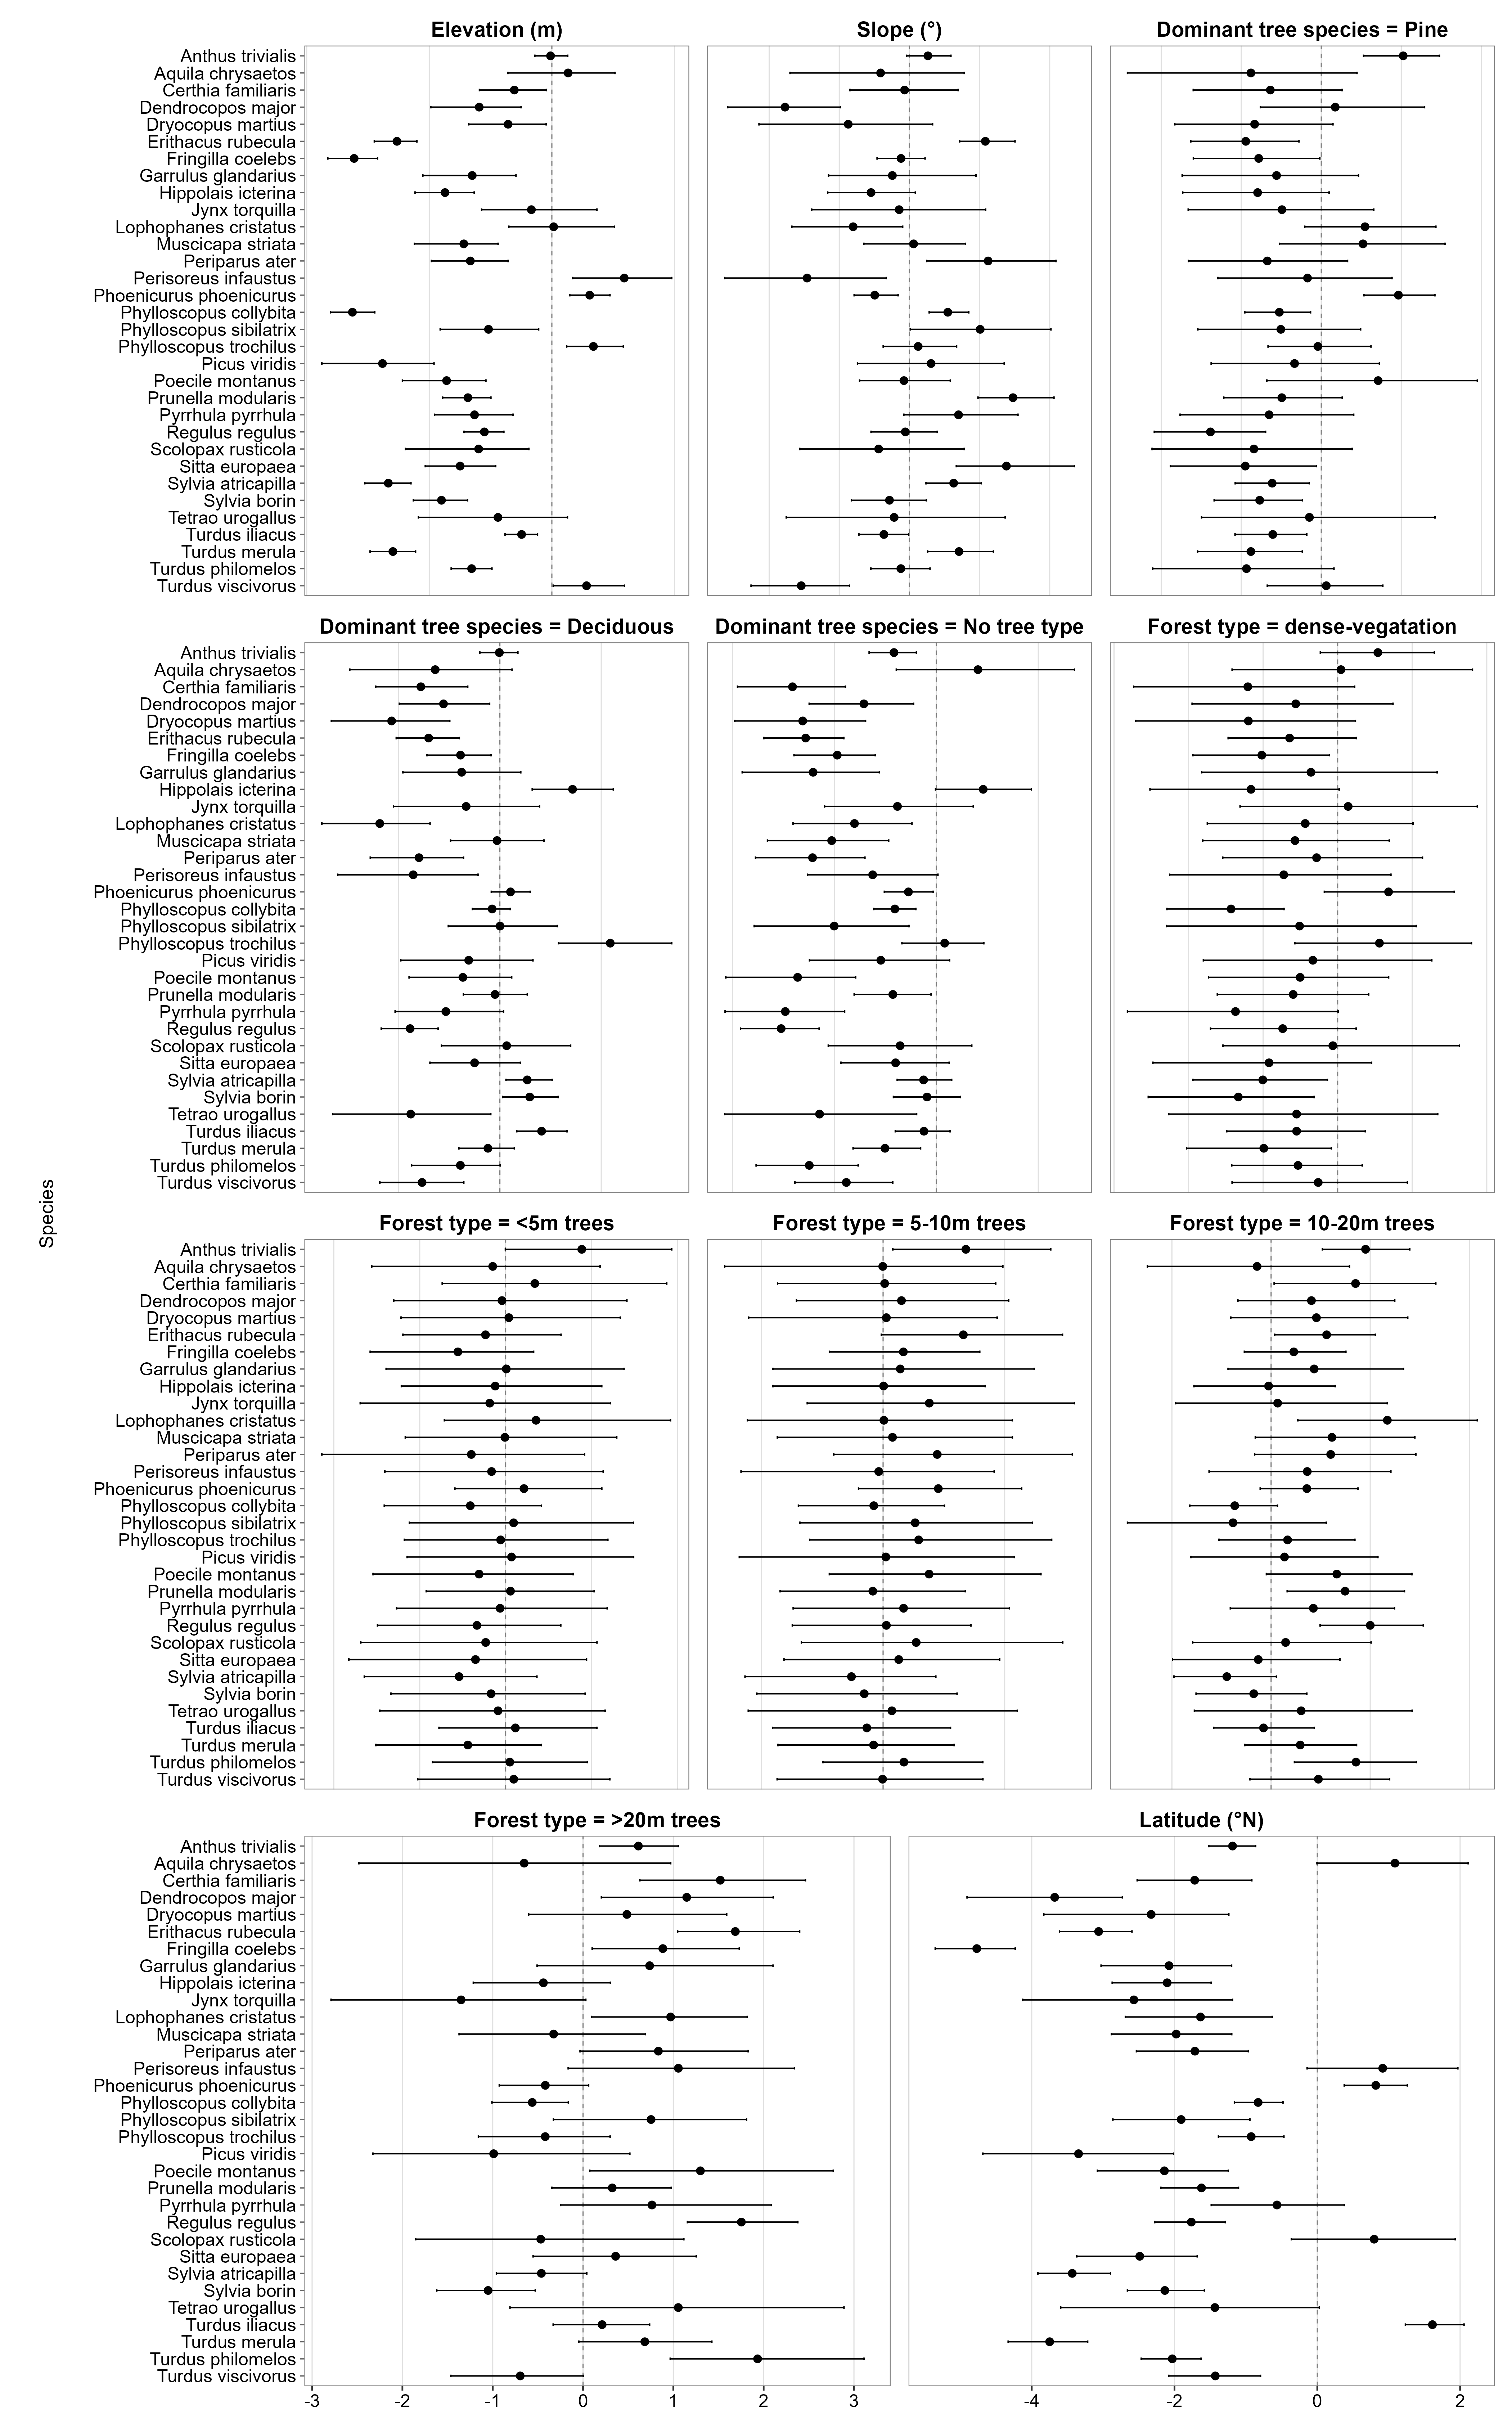
\includegraphics[width=1\linewidth,height=\textheight,keepaspectratio]{../img/forest/occupancy_effects.png}

}

\caption{\label{fig-forestOccEffs}Species-specific effects of
environmental and forest habitat covariates on occupancy in forest
ecosystems from the multi-species spatial model. Points are posterior
mean coefficient estimates (logit scale) and horizontal lines are the
corresponding uncertainty intervals. Estimates are shown for elevation,
slope, dominant tree species, forest type and latitude. The vertical
dashed line marks a coefficient of zero; estimates to either side
indicate negative and positive associations with occupancy,
respectively.}

\end{figure}%

For detection, the effect of temperature was positive for many species
(for example chaffinch, great spotted woodpecker, black woodpecker,
blackcap and common blackbird) and negative for a few (willow warbler
and marsh tit). Effects of precipitation were small and the intervals
overlapped zero for most species (Figure~\ref{fig-forestDetEffs}).

\begin{figure}

\centering{

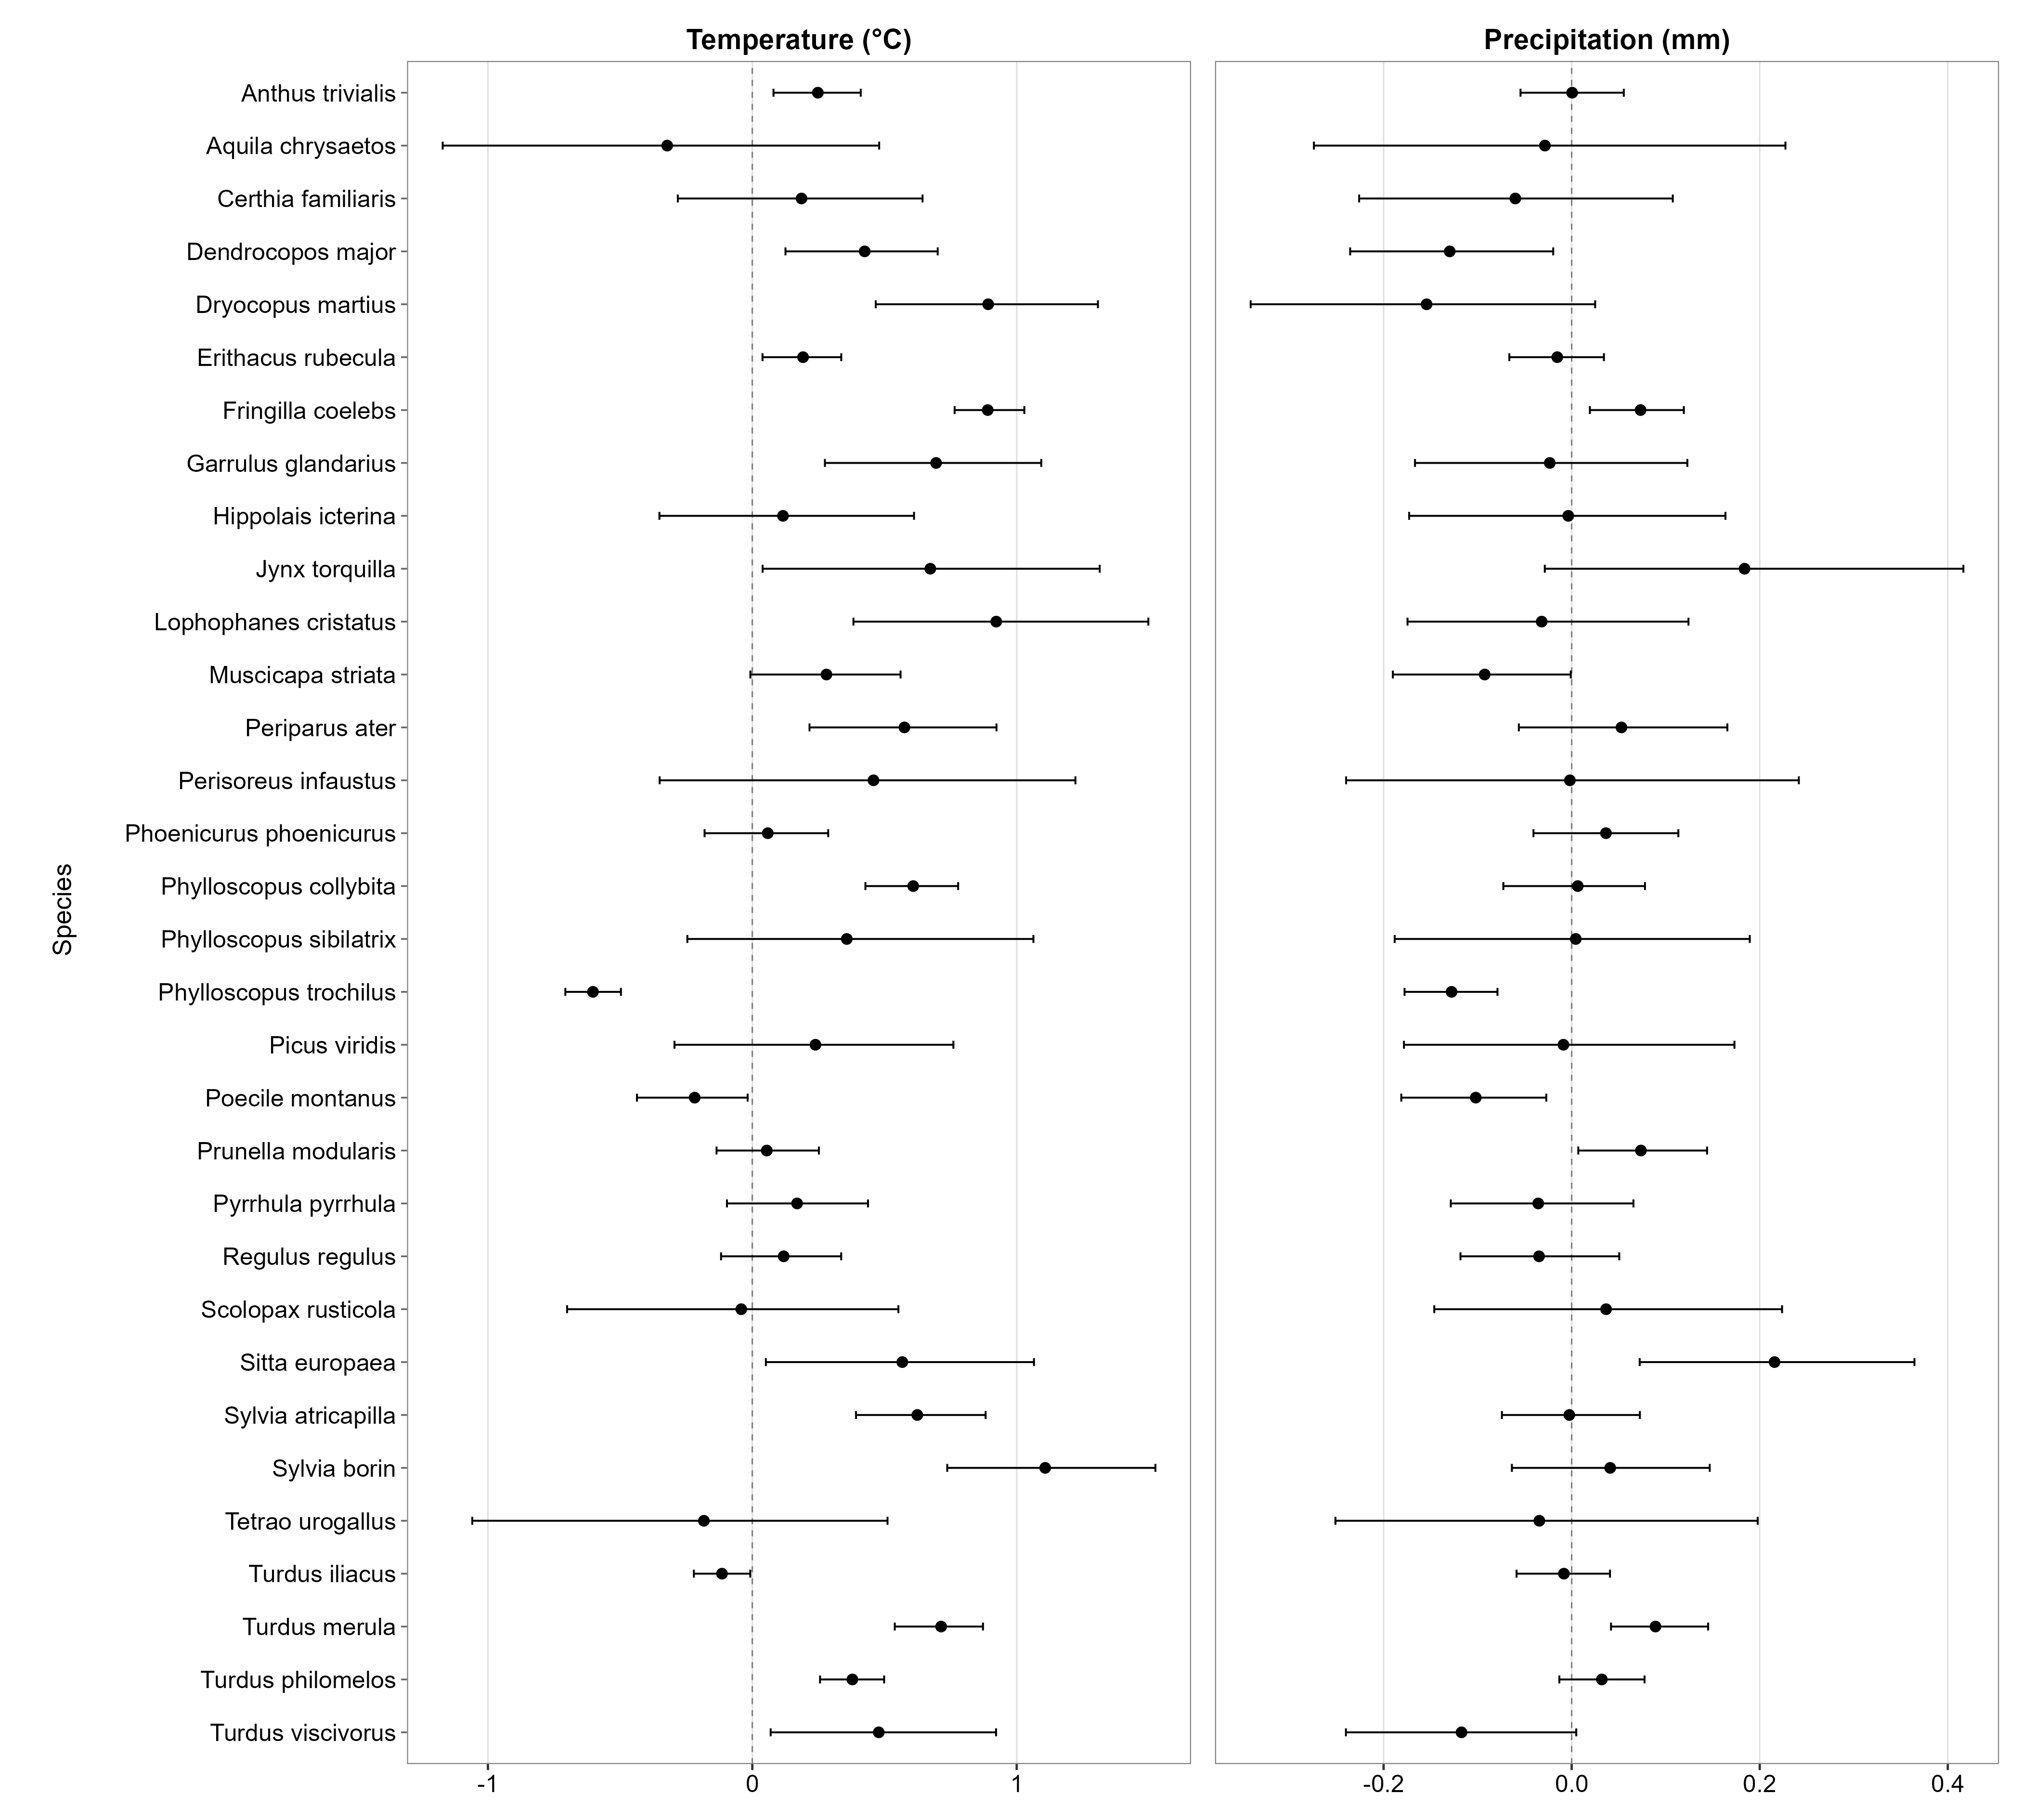
\includegraphics[width=1\linewidth,height=\textheight,keepaspectratio]{../img/forest/detection_effects.png}

}

\caption{\label{fig-forestDetEffs}Species-specific effects of
temperature and precipitation on detection probability in forest
ecosystems from the multi-species spatial model. Points are posterior
mean coefficient estimates (logit scale) and horizontal lines are the
corresponding uncertainty intervals. The vertical dashed line marks a
coefficient of zero.}

\end{figure}%

Estimated detection probabilities differed greatly among species
(Figure~\ref{fig-forestOccVrsDet}). Several species had very low
estimated detection per survey (about \(0.003\)--\(0.03\), for example
in golden eagle, wryneck, black grouse and green woodpecker), meaning
that their occupancy estimates rest heavily on model assumptions and are
weakly informed by data. For some very widespread species (such as
willow warbler and chaffinch), occupancy was estimated close to \(1\).

\begin{figure}

\centering{

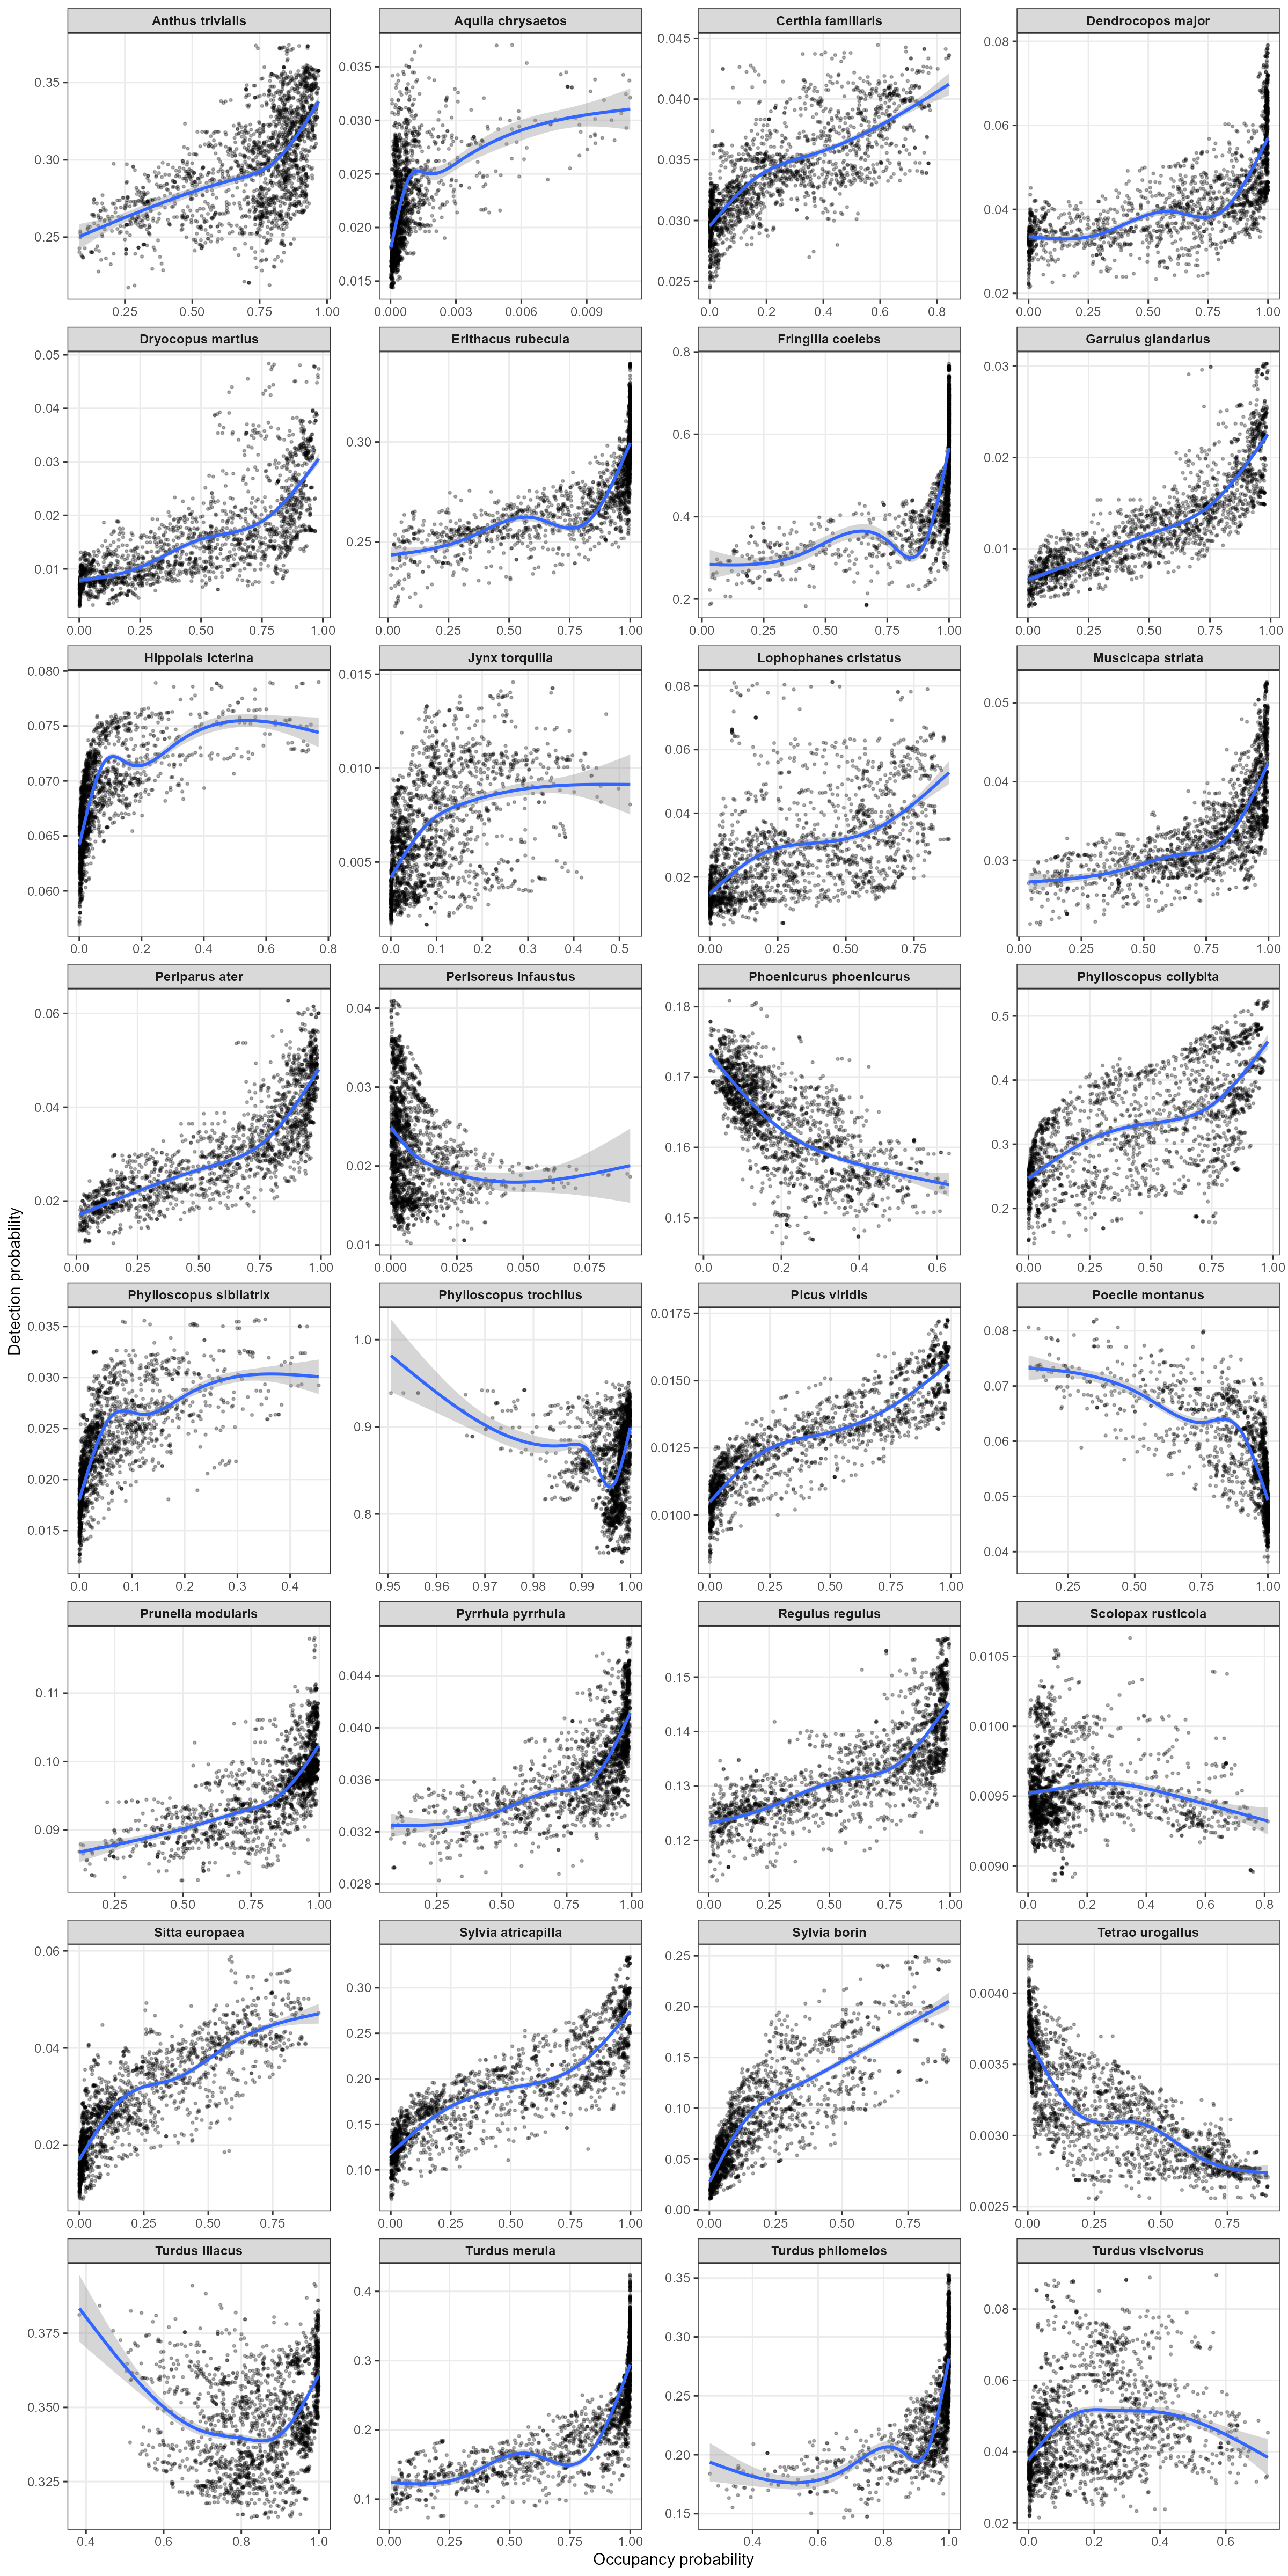
\includegraphics[width=1\linewidth,height=\textheight,keepaspectratio]{../img/forest/multi_species_detection_vs_occupancy.png}

}

\caption{\label{fig-forestOccVrsDet}Relationship between estimated
detection probability and occupancy probability for each forest species
at the prediction locations. Each point is a location and the blue line
is a smoothed trend. Note that the vertical scale differs among
species.}

\end{figure}%

\paragraph{10.3.2 Mountain ecosystem}\label{mountain-ecosystem}

For occupancy, elevation had a negative effect on most mountain species,
with the strongest negative effects for willow ptarmigan, bluethroat and
ring ouzel, whereas rock ptarmigan and snow bunting \emph{Plectrophenax
nivalis} showed positive or neutral effects
(Figure~\ref{fig-mountainOccEffs}). Latitude had positive effects for
most species. Effects of distance to the tree line and distance to wind
farms differed in direction among species, and for several species the
intervals were wide. The effect of distance to wind farms should be
regarded as descriptive, because wind farms are not randomly located
relative to habitat.

\begin{figure}

\centering{

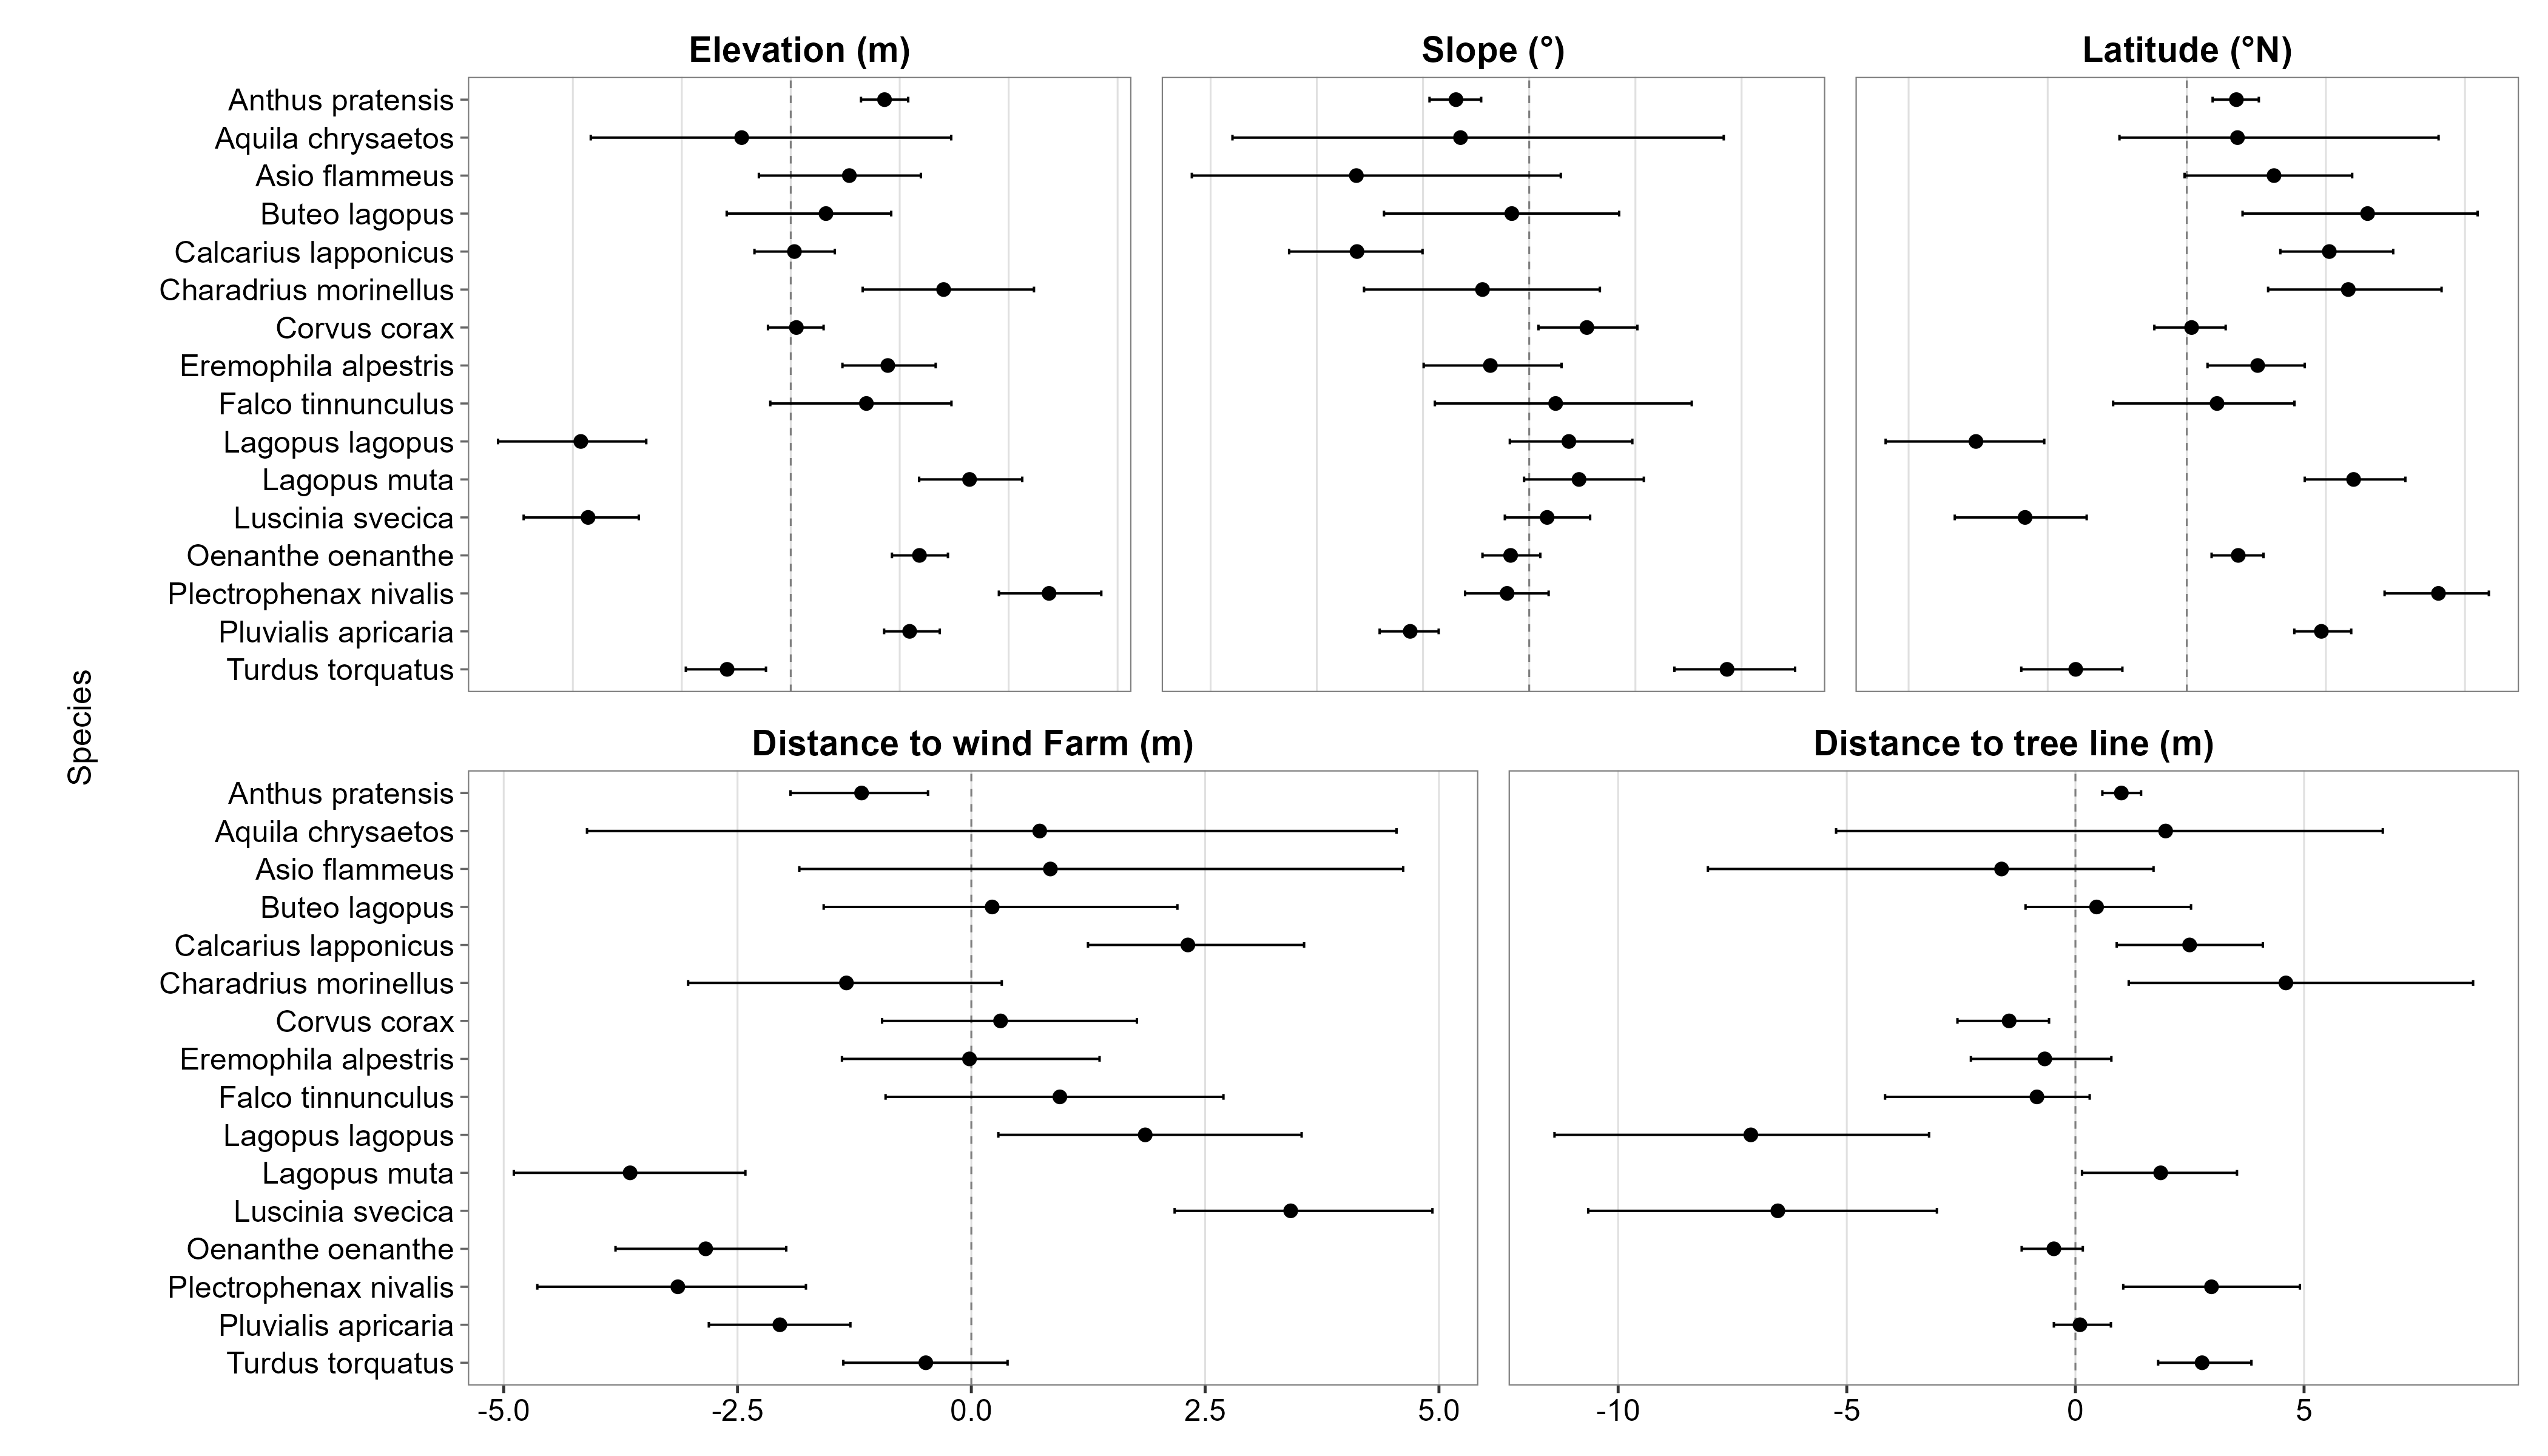
\includegraphics[width=1\linewidth,height=\textheight,keepaspectratio]{../img/mountain/occupancy_effects.png}

}

\caption{\label{fig-mountainOccEffs}Species-specific effects of
environmental covariates on occupancy in mountain ecosystems from the
multi-species spatial model. Points are posterior mean coefficient
estimates (logit scale) and horizontal lines are the corresponding
uncertainty intervals. Estimates are shown for elevation, slope,
latitude, distance to wind farm and distance to tree line. The vertical
dashed line marks a coefficient of zero.}

\end{figure}%

For detection, temperature had positive effects for some species (common
raven, rough-legged buzzard, common kestrel) and negative effects for
others (willow ptarmigan, bluethroat, northern wheatear and Eurasian
dotterel). Precipitation effects were generally small or negative
(Figure~\ref{fig-mountainDetEffs}). Detection probabilities were very
low for most raptors and owls (about \(0.001\)--\(0.01\) for golden
eagle, short-eared owl, rough-legged buzzard and common kestrel), so
occupancy for these species is weakly informed by the data
(Figure~\ref{fig-mountainOccVrsDet}).

\begin{figure}

\centering{

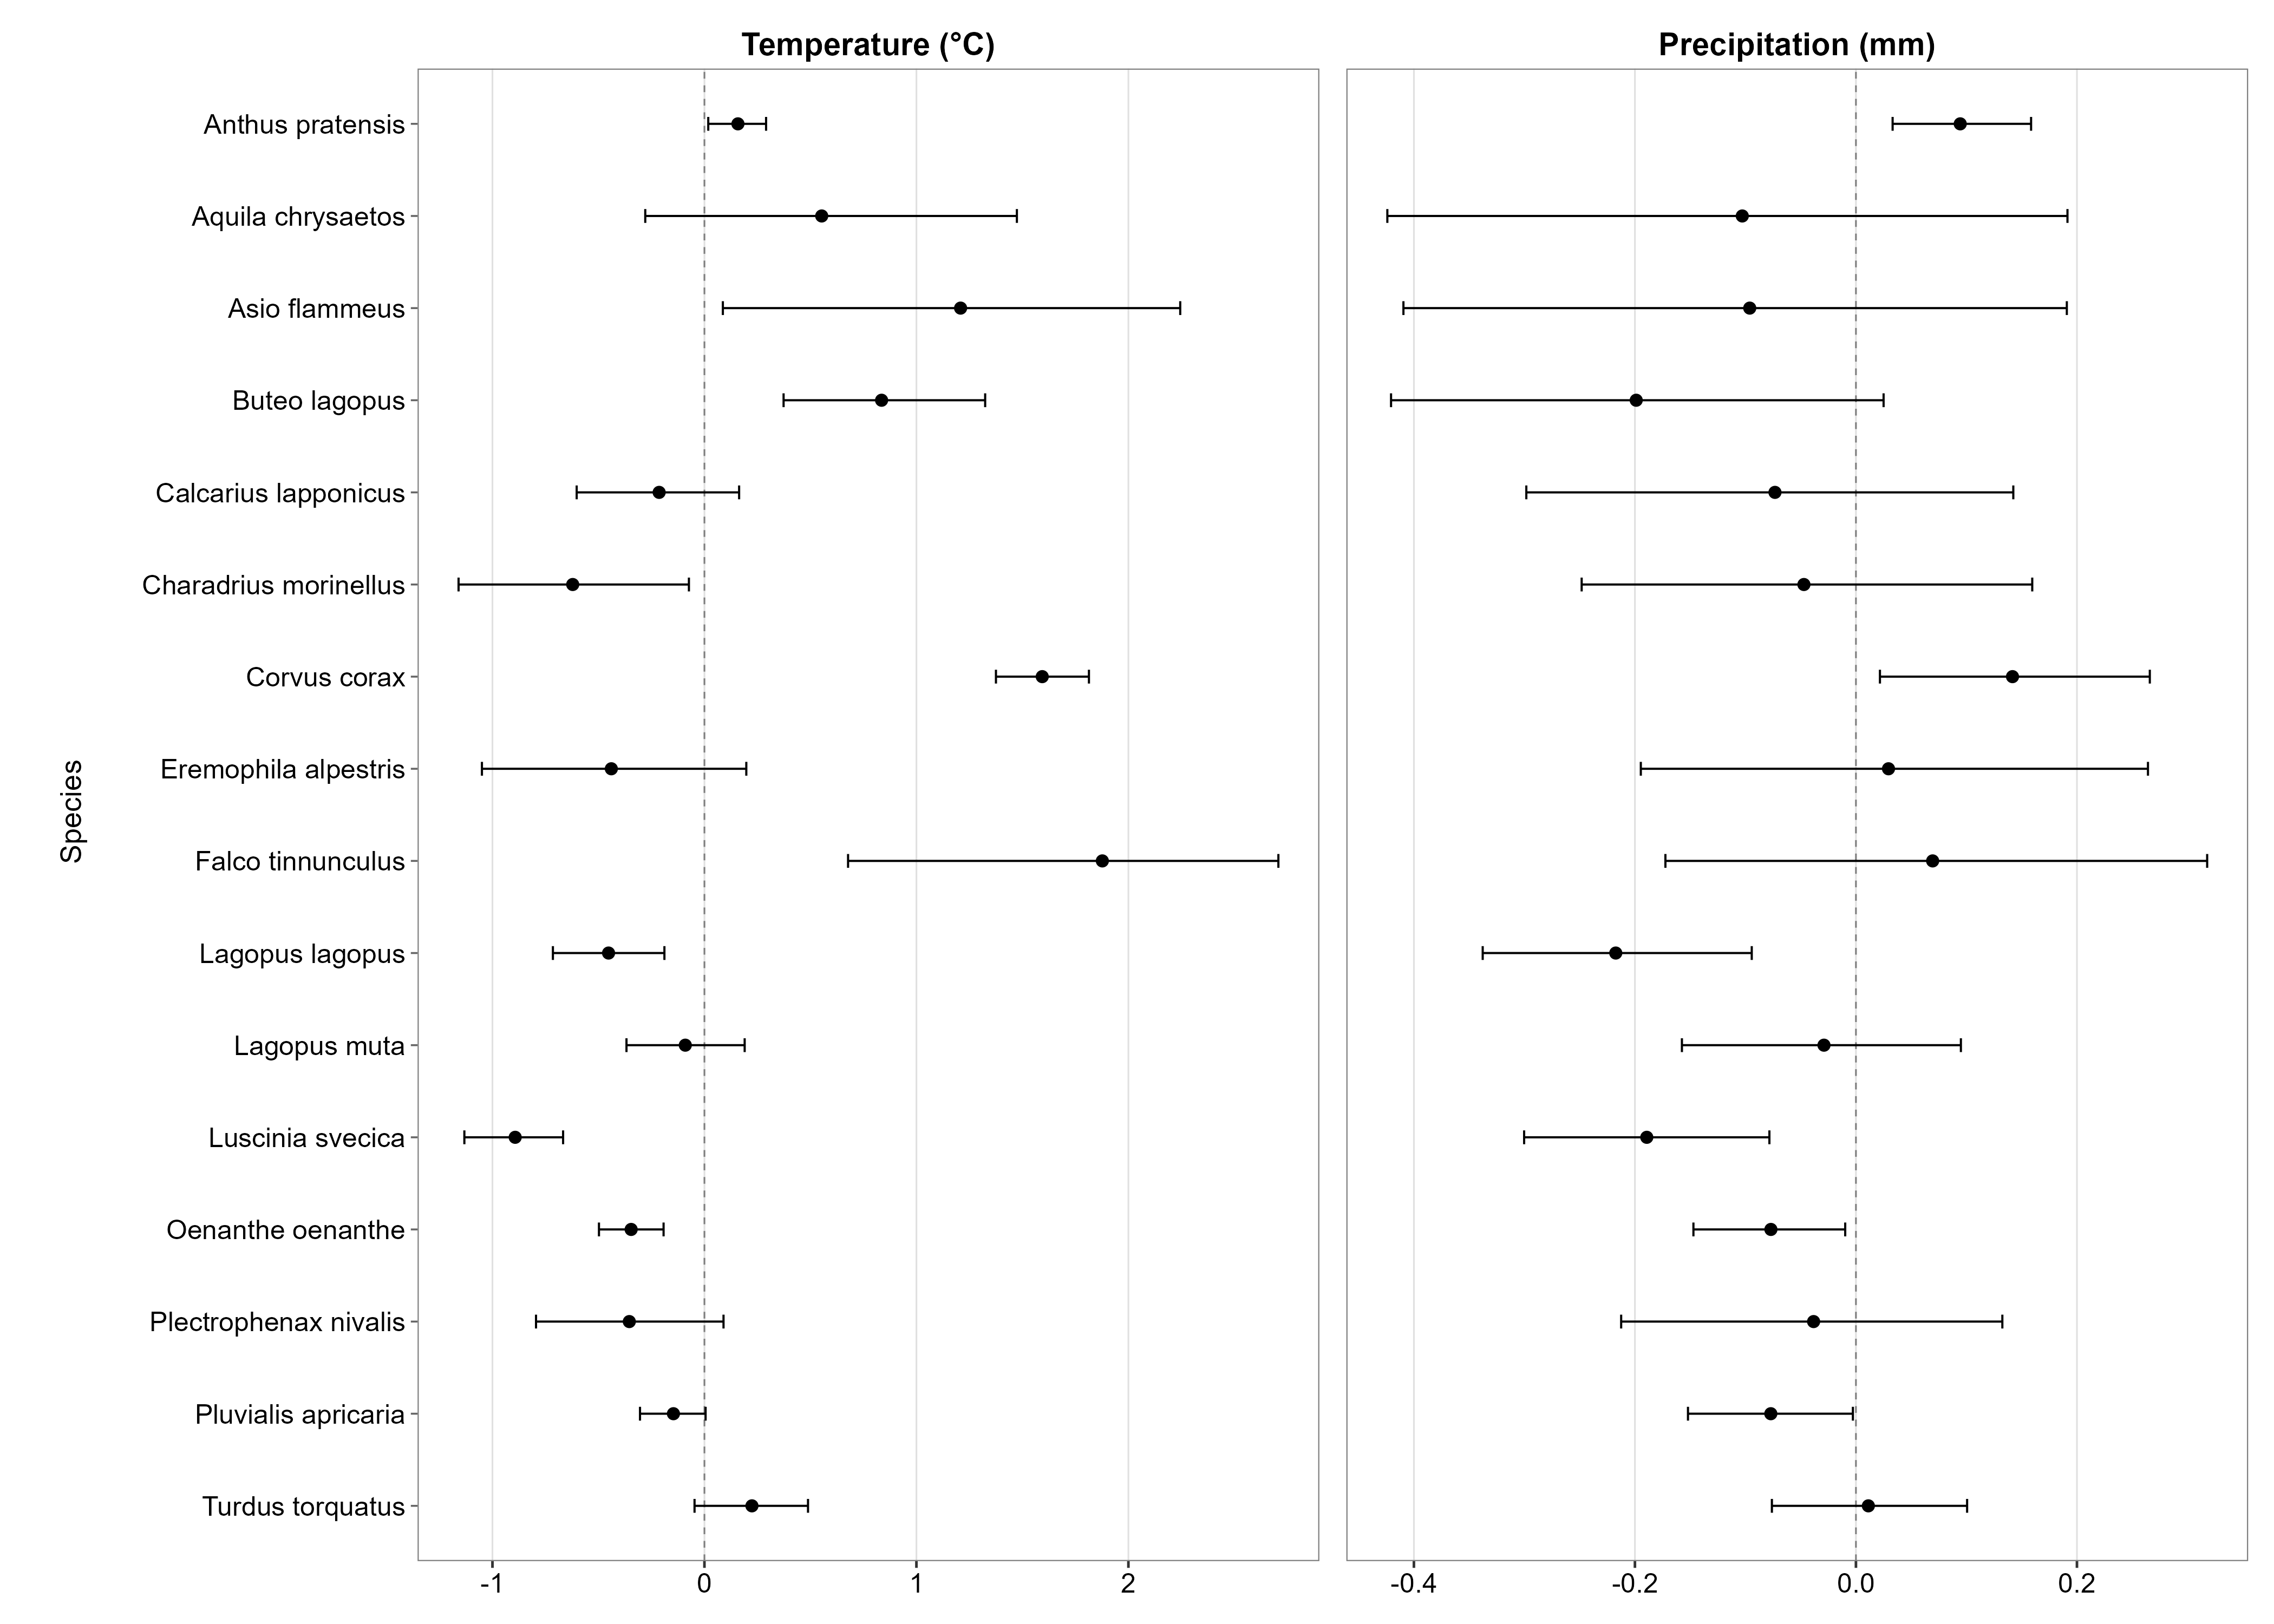
\includegraphics[width=1\linewidth,height=\textheight,keepaspectratio]{../img/mountain/detection_effects.png}

}

\caption{\label{fig-mountainDetEffs}Species-specific effects of
temperature and precipitation on detection probability in mountain
ecosystems from the multi-species spatial model. Points are posterior
mean coefficient estimates (logit scale) and horizontal lines are the
corresponding uncertainty intervals. The vertical dashed line marks a
coefficient of zero.}

\end{figure}%

\begin{figure}

\centering{

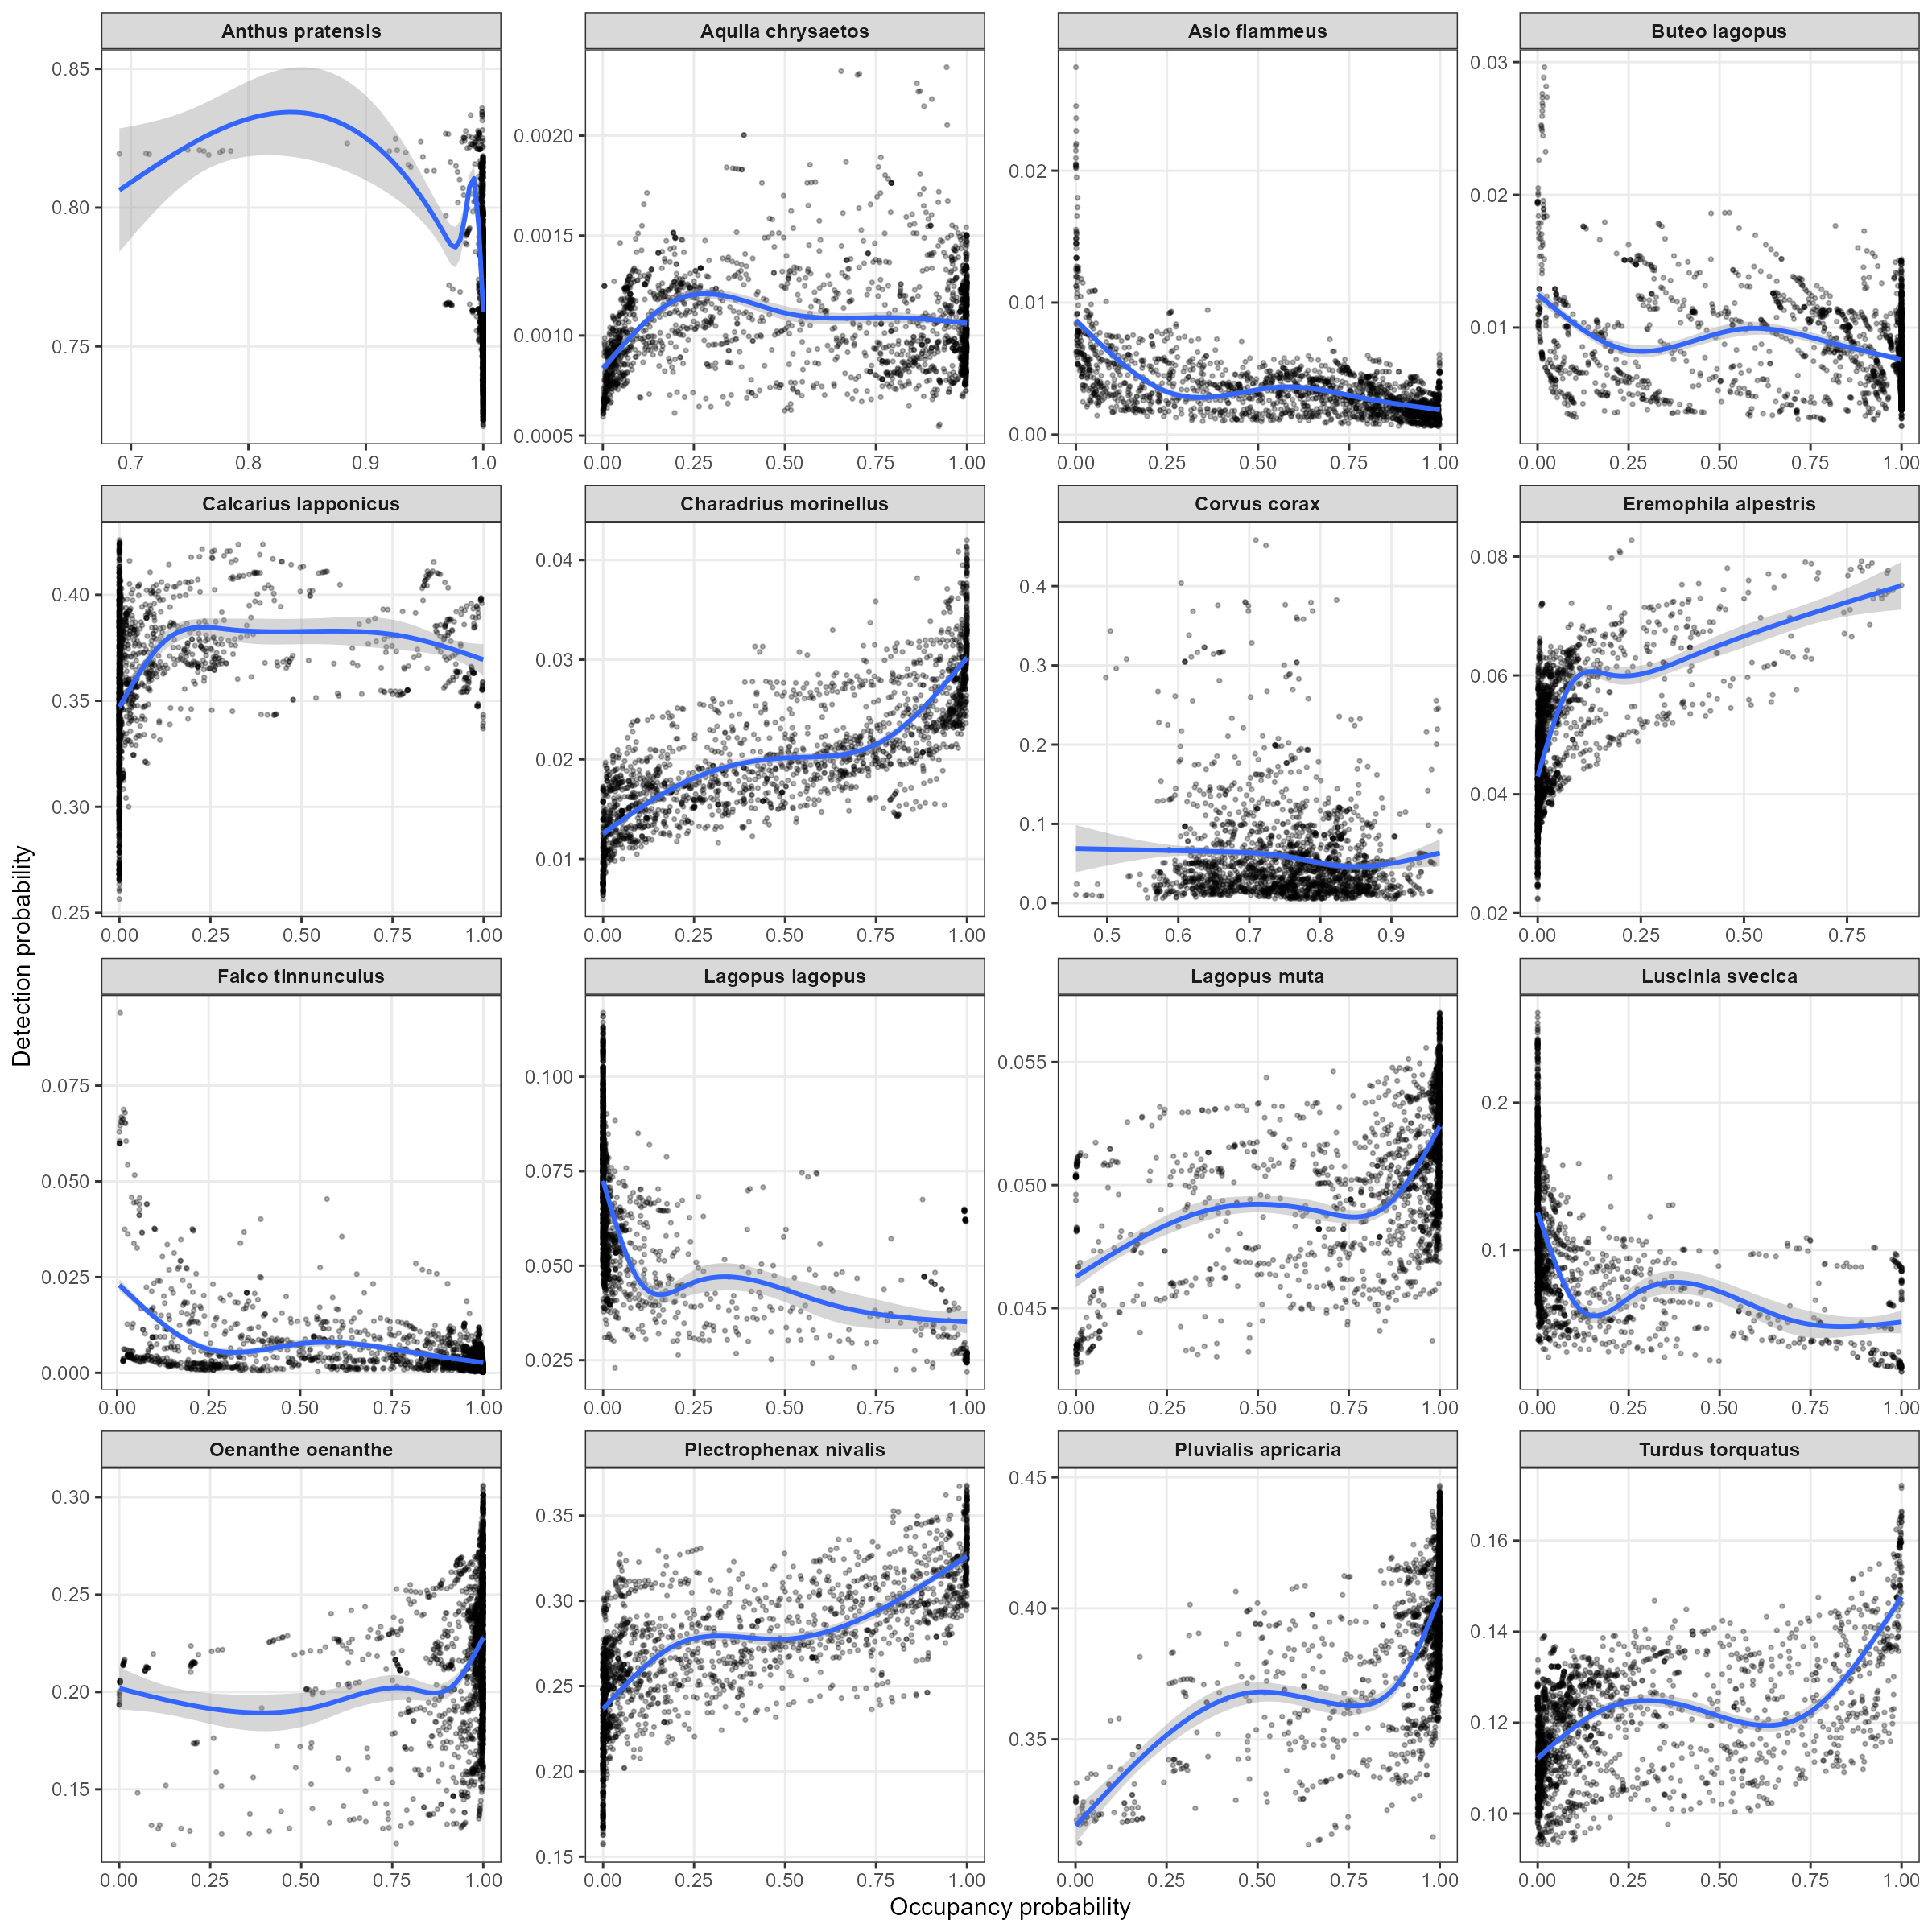
\includegraphics[width=1\linewidth,height=\textheight,keepaspectratio]{../img/mountain/multi_species_detection_vs_occupancy.png}

}

\caption{\label{fig-mountainOccVrsDet}Relationship between estimated
detection probability and occupancy probability for each mountain
species at the prediction locations. Each point is a location and the
blue line is a smoothed trend. Note that the vertical scale differs
among species.}

\end{figure}%

\subsubsection{10.4 Model selection and fit}\label{sec-modelSelection}

The multi-species spatial occupancy model was selected for both forest
and mountain ecosystems (selection procedure in Section 9.1.2).

Model fit was checked with Bayesian p-values for each species, where
values near \(0.5\) indicate adequate fit and values close to \(0\) or
\(1\) indicate that the model does not reproduce the data well
(Figure~\ref{fig-forestPPC}, Figure~\ref{fig-mountainPPC}). Fit was
adequate for most species but not all. In forest, seven of the 32
species had p-values below \(0.05\) (chaffinch \emph{Fringilla coelebs},
willow warbler \emph{Phylloscopus trochilus}, tree pipit \emph{Anthus
trivialis}, European robin \emph{Erithacus rubecula}, and three
thrushes: \emph{Turdus iliacus}, \emph{T. merula}, \emph{T.
philomelos}). In mountain, five of the 16 species had p-values below
\(0.05\) (meadow pipit \emph{Anthus pratensis}, European golden plover
\emph{Pluvialis apricaria}, ring ouzel \emph{Turdus torquatus}, willow
ptarmigan \emph{Lagopus lagopus} and northern wheatear \emph{Oenanthe
oenanthe}). No species had p-values above \(0.7\). Most of the poorly
fitting species are common and widespread, and for several of them the
model predicts occupancy close to \(1\) across much of the ecosystem.
Occupancy estimates for these species are therefore less reliable than
for the rest of the community.

\begin{figure}

\centering{

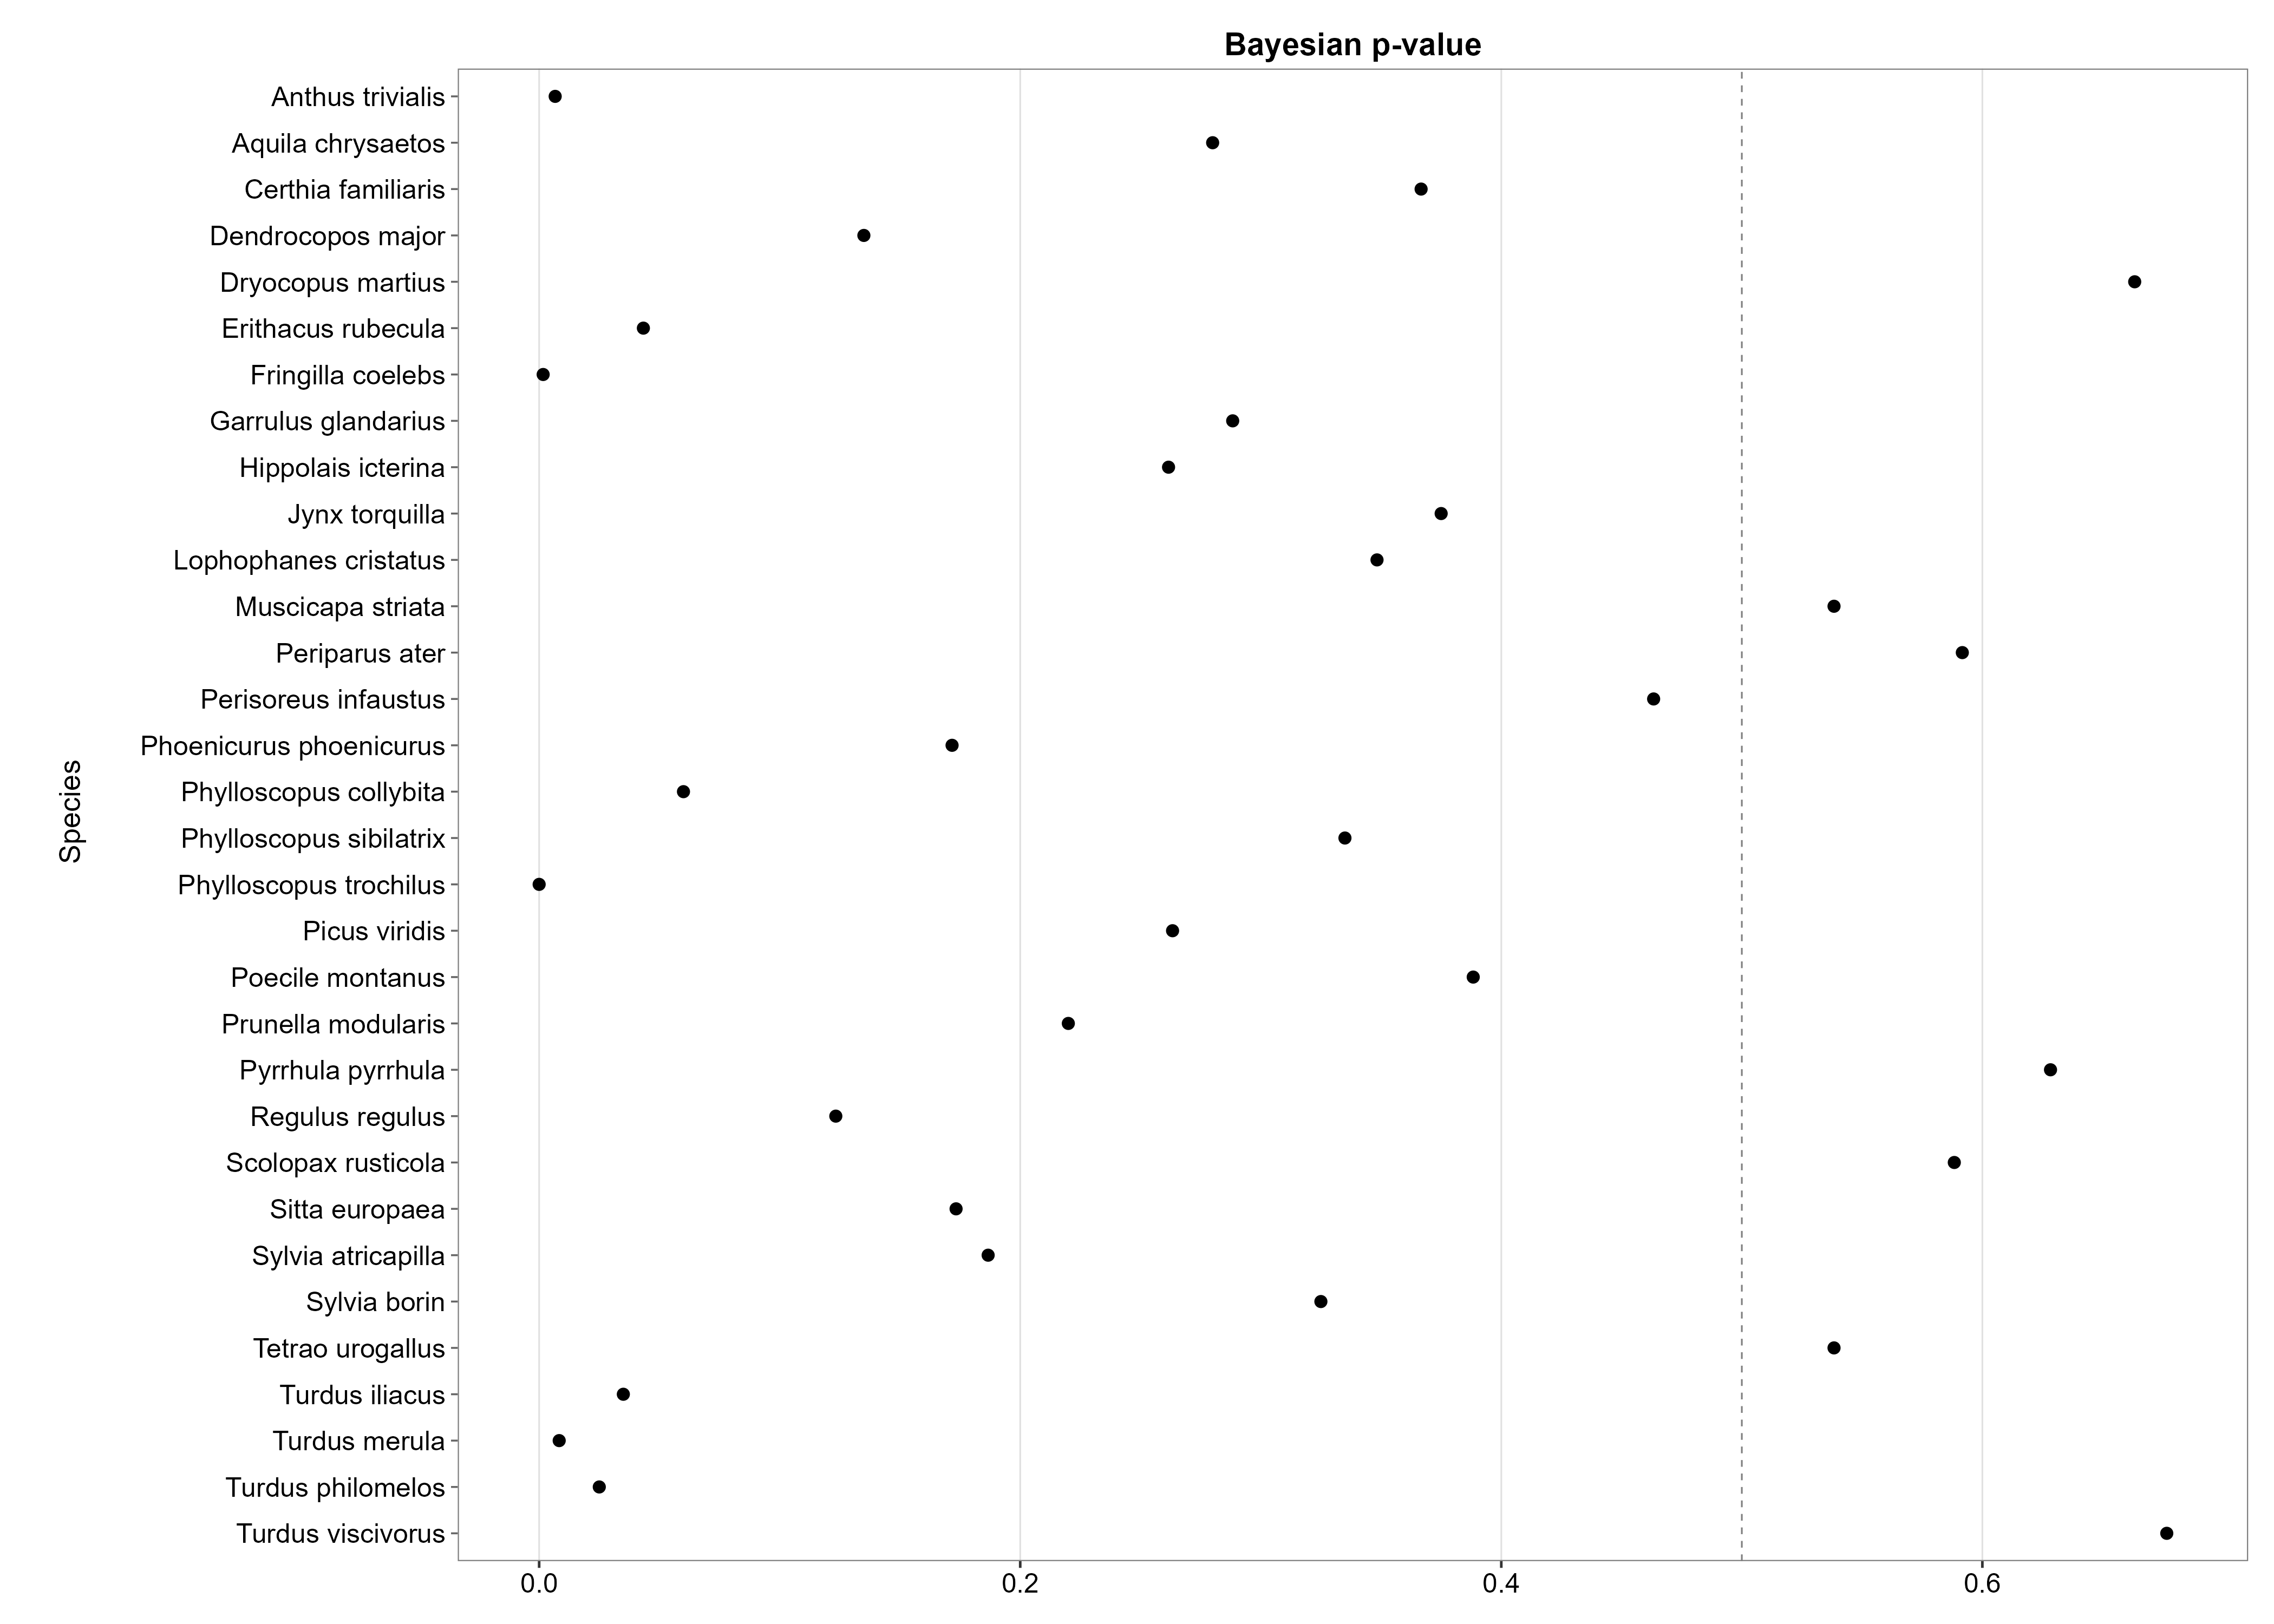
\includegraphics[width=1\linewidth,height=\textheight,keepaspectratio]{../img/forest/posterior_predictive_checks.png}

}

\caption{\label{fig-forestPPC}Posterior predictive checks for the forest
multi-species occupancy model. Each point is the Bayesian p-value for
one species. The dashed line marks 0.5, which indicates adequate fit;
values close to 0 indicate that the model does not reproduce the
observed data for that species.}

\end{figure}%

\begin{figure}

\centering{

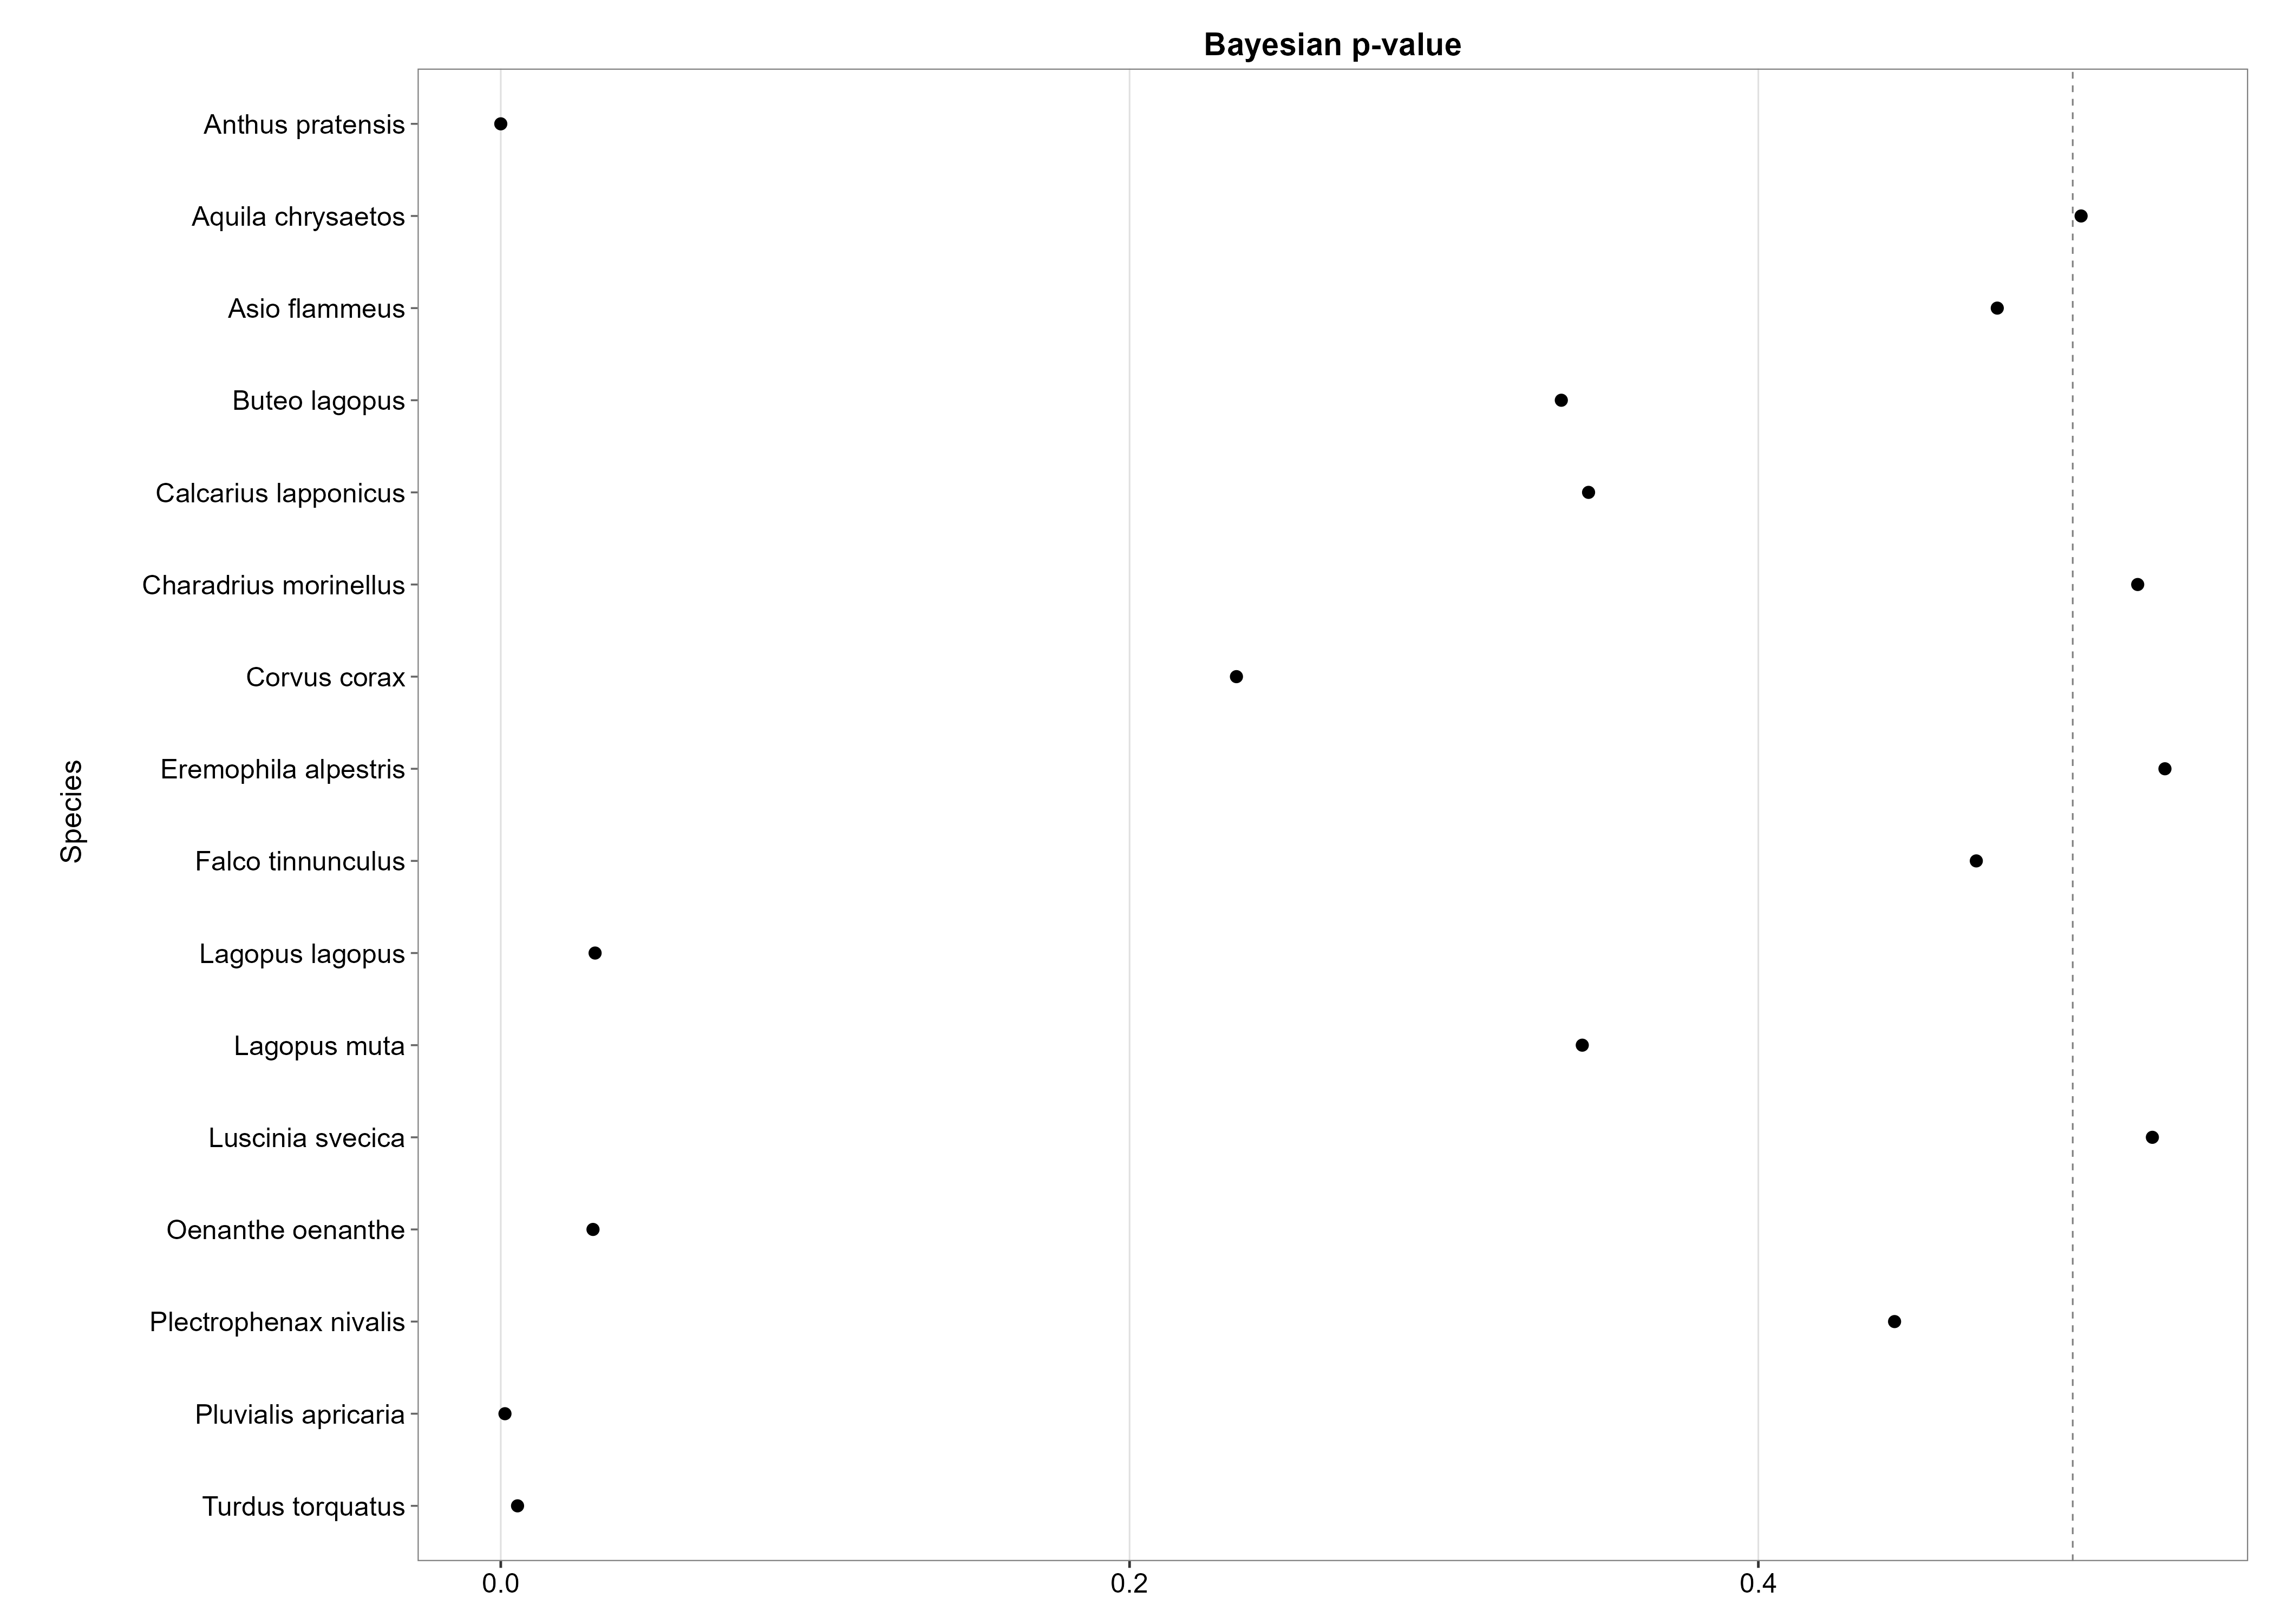
\includegraphics[width=1\linewidth,height=\textheight,keepaspectratio]{../img/mountain/posterior_predictive_checks.png}

}

\caption{\label{fig-mountainPPC}Posterior predictive checks for the
mountain multi-species occupancy model. Each point is the Bayesian
p-value for one species. The dashed line marks 0.5, which indicates
adequate fit; values close to 0 indicate that the model does not
reproduce the observed data for that species.}

\end{figure}%

\subsection{11. Export file}\label{export-file}

\subsection{12. Author contributions}\label{author-contributions}

\textbf{CRediT statement}

\begin{itemize}
\tightlist
\item
  Conceptualization: {[}KPA, Initials{]}
\item
  Methodology: {[}KPA, Initials{]}
\item
  Data curation: {[}Initials{]}
\item
  Formal analysis: {[}KPA, Initials{]}
\item
  Investigation: {[}KPA, Initials{]}
\item
  Software: {[}KPA, Initials{]}
\item
  Validation: {[}KPA, Initials{]}
\item
  Visualization: {[}KPA, Initials{]}
\item
  Resources: {[}Initials{]}
\item
  Writing -- original draft: {[}KPA, Initials{]}
\item
  Writing -- review \& editing: {[}Initials{]}
\item
  Supervision: {[}Initials{]}
\item
  Project administration: {[}Initials{]}
\item
  Funding acquisition: {[}Initials{]}
\end{itemize}

\textbf{MeRIT attribution}

This part supplements the CRediT statement with more granularity for
method section.

\textbf{Study design} The study was designed by {[}AB, CD{]}.

\textbf{Data collection / fieldwork} Field data were collected by {[}AB,
EF{]} between {[}years{]}. Sampling protocol was developed by {[}CD{]}.

\textbf{Laboratory procedures} DNA extraction was performed by {[}GH{]}.
Sequencing was conducted by {[}IJ{]}.

\textbf{Data processing} Raw data were curated and cleaned by {[}DPJ{]}.
Code for preprocessing was written by {[}KL{]}.

\textbf{Statistical analysis} All analyses were conducted by {[}KPA, {]}
using \texttt{spOccupancy}, with verification by {[}AB{]}.

\textbf{Visualization} Figures were produced by {[}KPA, {]}, with input
from {[}CD{]}.

\textbf{Reproducibility} All code was reviewed and validated by {[}AB,
CD{]}.

\begin{tcolorbox}[enhanced jigsaw, arc=.35mm, bottomrule=.15mm, bottomtitle=1mm, breakable, colback=white, colbacktitle=quarto-callout-tip-color!10!white, colframe=quarto-callout-tip-color-frame, coltitle=black, left=2mm, leftrule=.75mm, opacityback=0, opacitybacktitle=0.6, rightrule=.15mm, title={Session Info}, titlerule=0mm, toprule=.15mm, toptitle=1mm]

This information is mainly aimed at developers that need to recreate the
R environment that produced the html. Important note: this information
is about the R session that was running when the html was rendered, and
if some of the code chunks were not evaluated when the html was
rendered, they may have been executed in a different environment.

\begin{verbatim}
R version 4.6.0 (2026-04-24 ucrt)
Platform: x86_64-w64-mingw32/x64
Running under: Windows 11 x64 (build 26200)

Matrix products: default
  LAPACK version 3.12.1

locale:
[1] LC_COLLATE=Norwegian Bokmål_Norway.utf8 
[2] LC_CTYPE=Norwegian Bokmål_Norway.utf8   
[3] LC_MONETARY=Norwegian Bokmål_Norway.utf8
[4] LC_NUMERIC=C                            
[5] LC_TIME=Norwegian Bokmål_Norway.utf8    

time zone: Europe/Oslo
tzcode source: internal

attached base packages:
[1] stats     graphics  grDevices utils     datasets  methods   base     

other attached packages:
 [1] conflicted_1.2.0 yaml_2.3.12      anybadger_0.1.1  here_1.0.2      
 [5] kableExtra_1.4.1 lubridate_1.9.5  forcats_1.0.1    stringr_1.6.0   
 [9] dplyr_1.2.1      purrr_1.2.2      readr_2.2.0      tidyr_1.3.2     
[13] tibble_3.3.1     ggplot2_4.0.3    tidyverse_2.0.0  knitr_1.52      

loaded via a namespace (and not attached):
 [1] config_0.3.2       generics_0.1.4     xml2_1.6.0         stringi_1.8.9     
 [5] hms_1.1.4          digest_0.6.39      magrittr_2.0.5     evaluate_1.0.5    
 [9] grid_4.6.0         timechange_0.4.0   RColorBrewer_1.1-3 fastmap_1.2.0     
[13] cellranger_1.1.0   rprojroot_2.1.1    jsonlite_2.0.0     tinytex_0.61      
[17] viridisLite_0.4.3  scales_1.4.0       codetools_0.2-20   textshaping_1.0.5 
[21] cli_3.6.6          crayon_1.5.3       rlang_1.3.0        bit64_4.8.6       
[25] cachem_1.1.0       withr_3.0.3        otel_0.2.0         parallel_4.6.0    
[29] tools_4.6.0        tzdb_0.5.0         memoise_2.0.1      vctrs_0.7.3       
[33] R6_2.6.1           lifecycle_1.0.5    bit_4.6.0          vroom_1.7.1       
[37] pkgconfig_2.0.3    pillar_1.11.1      gtable_0.3.6       glue_1.8.1        
[41] systemfonts_1.3.2  xfun_0.61          tidyselect_1.2.1   rstudioapi_0.19.0 
[45] farver_2.1.2       htmltools_0.5.9    rmarkdown_2.32     svglite_2.2.2     
[49] compiler_4.6.0     S7_0.2.2           readxl_1.5.0      
\end{verbatim}

\end{tcolorbox}




\end{document}
